\documentclass[11pt,letterpaper]{article}
\usepackage[T1]{fontenc}
\usepackage{lmodern}
\usepackage[margin=1in]{geometry}
\usepackage{amsmath,amssymb,amsthm,mathtools,bm}
\usepackage{enumitem,microtype,booktabs}
\usepackage{tikz}
\usetikzlibrary{arrows.meta,positioning,calc,decorations.pathreplacing,patterns}
\usepackage[colorlinks=true,linkcolor=blue!45!black,citecolor=blue!45!black,urlcolor=blue!45!black]{hyperref}
\usepackage[capitalize,nameinlink,noabbrev]{cleveref}
\numberwithin{equation}{section}
\newtheorem{theorem}{Theorem}[section]
\newtheorem{lemma}[theorem]{Lemma}
\newtheorem{proposition}[theorem]{Proposition}
\newtheorem{corollary}[theorem]{Corollary}
\theoremstyle{definition}
\newtheorem{definition}[theorem]{Definition}
\newtheorem{remark}[theorem]{Remark}
\newtheorem{convention}[theorem]{Convention}
\newcommand{\N}{\mathbb N}
\newcommand{\Z}{\mathbb Z}
\newcommand{\R}{\mathbb R}
\newcommand{\C}{\mathbb C}
\newcommand{\Torus}{\mathbb T}
\newcommand{\E}{\mathbb E}
\newcommand{\Prob}{\mathbb P}
\newcommand{\ind}{\mathbf 1}
\newcommand{\eps}{\varepsilon}
\newcommand{\ee}[1]{e\!\left(#1\right)}
\newcommand{\abs}[1]{\lvert #1\rvert}
\newcommand{\norm}[1]{\lVert #1\rVert}
\newcommand{\Pplus}{P^{+}}
\newcommand{\Pminus}{P^{-}}
\DeclareMathOperator{\supp}{supp}
\DeclareMathOperator{\lcm}{lcm}
\DeclareMathOperator{\Li}{Li}
\DeclareMathOperator{\id}{id}
\DeclareMathOperator{\rank}{rank}
\setlist[enumerate]{label=\textup{(\roman*)},leftmargin=*}
\setlist[itemize]{leftmargin=*}
\setlength{\emergencystretch}{1em}
\setcounter{tocdepth}{1}
\hypersetup{
  pdftitle={Weighted dilation graphs, smooth shifted primes and totient fibers},
  pdfauthor={OpenAI},
  pdfsubject={Smooth predecessors of primes and totient multiplicities}
}
\makeatletter
\renewcommand{\@maketitle}{%
  \newpage\null\vskip 1em
  \begin{center}
    {\LARGE\@title\par}\vskip 1em
    {\large\@author\par}\vskip .5em
    {\@date\par}
  \end{center}
  \vskip 1em
}
\makeatother

\title{Weighted dilation graphs, smooth shifted primes and totient fibers}
\author{OpenAI}
\date{September 24, 2026}
\begin{document}
\maketitle
\begin{abstract}
We prove Erd\H{o}s's conjecture on the largest fibers of Euler's totient function: for every $\eps>0$, infinitely many positive integers $n$ have more than $n^{1-\eps}$ preimages. We also show that, for every fixed $\delta>0$, there are at least $x^{1-o(1)}$ primes $p$ in $2x<p\le5x$ whose predecessors have no prime factor exceeding $x^\delta$.
\end{abstract}
\section{Introduction}\label{sec:introduction}

Euler's totient function can take the same value at many different
integers. Write
\[
 g(n)=\#\{m\ge1:\varphi(m)=n\}
\]
for the size of its fiber at $n$. We prove the following result.

\begin{theorem}\label{thm:totient}
For every real $\eps>0$, there are infinitely many positive integers
$n$ such that
\[
 g(n)>n^{1-\eps}.
\]
\end{theorem}

\Cref{thm:totient} resolves positively Erd\H{o}s's conjecture on the
largest fibers of Euler's totient function. Pomerance
\cite[p.~84]{Pomerance1980} formulates the conjecture as $C=1$, where
$C$ is the supremum of the exponents $c$ for which $g(n)>n^c$ infinitely
often, and attributes it to Erd\H{o}s \cite{Erdos1956}. An elementary
upper bound is $g(n)\ll_\eta n^{1+\eta}$ for every $\eta>0$; we recall
it in \Cref{sec:totients}. Thus the power exponent of $n$ in the theorem is
optimal.

The arithmetic input is a result about the prime factors of the
predecessor of a prime. For $m>1$, let $P^+(m)$ be its largest prime
factor. Erd\H{o}s's work on totient multiplicities and smooth shifted
primes dates to \cite[Section~3]{Erdos1935}. The underlying
construction takes products of many primes whose predecessors have
few available prime factors: many distinct products then have the same
totient. The expectation that $p-1$ can have
all its prime factors smaller than every fixed power of $p$ was
recorded in \cite{Erdos1956}; see also
\cite[Introduction]{Lichtman2022}. We prove a quantitative form.

\begin{theorem}\label{thm:smooth}
For every fixed $0<\delta<1/4$, as $x\to\infty$,
\begin{equation}\label{eq:main-smooth}
 \#\{p:\ p\text{ prime},\ 2x<p\le5x,
                   \ P^+(p-1)\le x^\delta\}
 \ge x^{1-o(1)}.
\end{equation}
The quantity $o(1)$ may depend on $\delta$.
\end{theorem}

In particular, for every $\eps>0$ there are infinitely many primes
$p$ with $P^+(p-1)\le p^\eps$. This resolves the smooth-predecessor
conjecture positively as well. The count in \Cref{eq:main-smooth}
also holds for every fixed $\delta>0$, by using a smaller positive
exponent when necessary. No uniformity as $\delta\to0$ is
asserted in \Cref{thm:smooth} or needed for \Cref{thm:totient}.

There is a substantial literature on fixed smoothness exponents.
Baker and Harman \cite[Section~1, Theorem~1 and Corollary~1]{BakerHarman1998}
obtained exponent $0.2961$ for shifted primes, with the corresponding
totient multiplicity exponent $0.7039$. This improved Friedlander's
threshold $1/(2\sqrt e)+\eps$; their introduction also describes
preceding work of Pomerance, Balog, and Fouvry--Grupp.
Lichtman \cite[Theorem~1.1 and Corollary~1.3]{Lichtman2022}
proved a lower bound $x/(\log x)^C$ for $x<p\le2x$ and
$P^+(p-1)\le x^\beta$ whenever
\[
 \beta>\frac{15}{32\sqrt e}=0.284311\ldots,
\]
and obtained multiplicity exponent $0.7156$.
These results concern fixed positive exponents. The expected
Dickman law predicts a positive proportion of primes for every such
exponent; see Granville \cite[Section~5.3]{Granville2008}.
Bharadwaj and Rodgers \cite[Theorem~7, Proposition~2,
and Conjecture~5]{BharadwajRodgers2026} prove the full
Poisson--Dirichlet law for sequences satisfying their regularity and
congruence-uniformity conditions together with level-one distribution.
For shifted primes this gives the prediction under the
Elliott--Halberstam conjecture; their Proposition~2 establishes
distribution level one half and the other conditions unconditionally.
Our unconditional bound $x^{1-o(1)}$ gives the full power exponent of
the count for every fixed positive smoothness exponent. A positive
limiting proportion is a stronger conclusion.
The final passage from plentiful smooth shifted primes to large
totient fibers belongs to the method of Erd\H{o}s and Pomerance;
Pomerance states the relevant transfer explicitly in
\cite[Theorem~B]{Pomerance1980}. We give the needed
product-and-pigeonhole proof in full.

Smooth predecessors also enter the construction of Carmichael numbers
by Alford, Granville and Pomerance \cite{AlfordGranvillePomerance1994},
where their supply is combined with a separate distribution theorem
for primes in arithmetic progressions. This is one reason that
estimates for shifted smoothness have applications beyond the
factorization problem itself. The contribution here includes the
general graph and kernel theorems that produce the arithmetic lower
bound, as well as the optimal exponent for totient fibers.

These graph and ideal-kernel estimates also serve as inputs to the
companion paper \cite[Theorem~1.1]{PrimePredecessors}, where a separate
determinant-graph estimate and prime-extraction argument yield the full
Poisson--Dirichlet law for prime predecessors.

\subsection{The analytic mechanism}

The main obstacle is to detect primality in a sequence whose
predecessors have a strongly constrained factorization. Congruence
counts provide an initial sieve, and a further bilinear cancellation
estimate permits the composite contribution to be removed. This
division of work is familiar from prime-detecting sieves; compare
Friedlander and Iwaniec \cite[Section~1]{FriedlanderIwaniec1998}.
Our coefficient and range hypotheses are stated and verified below
for the particular weight used here.

We count primes of the form $2u+1$, where $u$ has a prescribed
factorization over many logarithmic scales. Some factors lie in
two separated ranges of subpower-sized primes, divided into small and
big groups. Their weights mark distinct prime divisors. The functions
attached to an integer depend only on the part of $u$ outside these
groups; the marked weights supply the divisibility
labels for the dilation graph. Other factors
occupy a geometric sequence of size bands, which permits a divisor
of $u$ to be chosen close to a specified size. One band contains a
long factor ranging over rough integers, meaning integers with no
prime factor below a prescribed cutoff.

The main new analytic ingredient is a transference theorem for
weighted dilation graphs. A physical state consists of an integer and
ordered lists of distinct group-prime divisors. An edge has shift
$kD$ for an integer $k\ne0$, where $D$ is a product of primes shared
by its endpoint lists,
together with independent free prime factors. The corresponding ideal
operator acts on the big-group lists: its labels are independent, with
probabilities proportional to $1/p$, and repetitions are allowed. The list length is sufficiently large
but fixed as $x$ tends to infinity. A small ideal operator norm yields
an averaged high moment of the physical graph, and hence cancellation
in pairings whose first endpoint is independent of its mark list.

The transference proof averages the integer root by the Chinese
remainder theorem. Repeated divisibility queries then pay a reciprocal
prime factor only once; a memory retains their congruences between
active uses. Averaging the omitted small marks makes transfers between
memory and the active lists rare. A rank expansion restores distinct
prime births while preserving cancellation on most edges: many
independent birth equalities supply reciprocal-prime savings, whereas
a small equality rank affects only a small fraction of the edges.
The theorem applies to arbitrary signed kernels satisfying its explicit
complexity and norm hypotheses.

Related divisibility-graph methods have a substantial history.
Matom\"aki, Radziwi\l\l{} and Tao
\cite[Theorem~5.1]{MatomakiRadziwillTao2016} studied connectivity
of a graph with prime-divisibility edges. Tao's entropy-decrement
argument \cite{Tao2016} replaces such divisibility conditions by
their mean at a suitable scale. Helfgott and Radziwi\l\l{}
\cite[Section~1.5]{HelfgottRadziwill2021} study centered adjacency
operators through signed closed-walk moments, with repeated primes
creating dependent congruences. Pilatte
\cite[Theorem~2.4 and Section~5]{Pilatte2026} develops this approach
for shifts that are products of primes. These works explain the
roles of centering, long moments, and repeated-label bookkeeping.
Our graph also carries ordered active lists, and its comparison
with an independent-label operator requires the explicit lifespan
and factorial-memory construction proved in \Cref{sec:transference}.

The independent-label norm is made small by a comparison construction.
Logarithmic localization and character kernels allow shared prime
products to be replaced by independent products. The big groups are
split into two blocks, with a bounded number of selected coordinates
in each group. After averaging the list coordinates unused by the
multiplier, a coordinate decomposition isolates components that have
mean zero in all selected coordinates of one block. Permutation
symmetry makes these components small, and signed comparison terms
cancel the other components up to a controlled error. For each
prescribed fixed accuracy, the construction gives kernels uniform in
the additive frequency, with complexity fixed
before the length of the marked lists is chosen.

Applying transference to the multiplicatively invariant endpoints
reduces a fixed shifted correlation to averages over larger shifts.
Products of free primes control the minor arcs. On the major arcs,
a marked small prime and the compulsory long rough-integer factor
control the local Fourier energy. A low-complexity character and
Mellin discrepancy condition supplies the remaining cancellation.
The argument permits arbitrary bounded residual coefficients.

These shifted correlations yield a Type II estimate for
$mn=2u+1$. A probabilistic split of the geometric prime bands chooses
a divisor $e$ of $u$ close to the scale of $m$. After Cauchy--Schwarz,
off-diagonal factorizations become shifted endpoints by an exact
determinant identity. The Type II estimate then permits primality
and roughness tests on cofactors to be replaced by elementary rough
proxies. Congruence estimates and a weighted sieve remove the
composite values of $2u+1$; a separate upper bound treats the small
balanced range.

\subsection{Organization and dependencies}

\Cref{sec:preliminaries} fixes the conventions and proves the
elementary sieve used later. The central transference estimate is
proved in \Cref{sec:transference}, and the independent-label kernels
are constructed in \Cref{sec:ideal}. Together they lead to the
shifted-correlation theorem in \Cref{sec:shifts}. The Type II
reduction occupies \Cref{sec:typeii}. The prime extraction and all
its parameter choices are completed in \Cref{sec:primes}.
\Cref{sec:totients} finishes the proof of \Cref{thm:totient}.
The main implications are summarized in \Cref{fig:proof-dependencies}.

The sieve geometry is fixed first, the required analytic accuracies
next, and the discrepancy precision of the cofactor proxies last.
The relevant theorems state this choice order, and the prime extraction
verifies it. In particular, the needed discrepancy is established
independently of the estimate that uses it.

\begin{figure}[!ht]
\centering
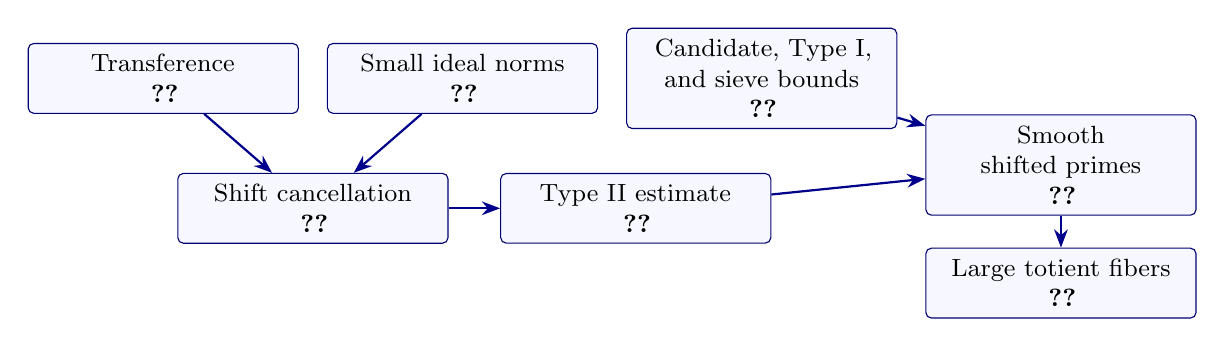
\begin{tikzpicture}[>=Stealth,
  box/.style={draw=blue!45!black,fill=blue!3,rounded corners=2pt,
              align=center,text width=3.15cm,minimum height=.78cm,
              inner sep=4pt,font=\small},
  link/.style={->,thick,draw=blue!55!black}]
 \node[box] (transfer) at (0,0)
   {Transference\\\Cref{thm:transference}};
 \node[box] (ideal) at (3.8,0)
   {Small ideal norms\\\Cref{thm:ideal}};
 \node[box] (shift) at (1.9,-1.65)
   {Shift cancellation\\\Cref{thm:shift}};
 \node[box] (typeii) at (6,-1.65)
   {Type II estimate\\\Cref{thm:typeii}};
 \node[box] (sieve) at (7.6,0)
   {Candidate, Type I,\\and sieve bounds\\\Cref{sec:primes}};
 \node[box] (smooth) at (11.4,-1.1)
   {Smooth shifted primes\\\Cref{thm:smooth}};
 \node[box] (totient) at (11.4,-2.6)
   {Large totient fibers\\\Cref{thm:totient}};
 \draw[link] (transfer)--(shift);
 \draw[link] (ideal)--(shift);
 \draw[link] (shift)--(typeii);
 \draw[link] (typeii)--(smooth);
 \draw[link] (sieve)--(smooth);
 \draw[link] (smooth)--(totient);
\end{tikzpicture}
\caption{Main result dependencies. The auxiliary branch includes
candidate mass, Type I distribution, proxy discrepancy, the elementary
sieve, and the separate balanced-range bound. Arrows record the implications used
in the proof; the order of choosing constants is described in the text.}
\label{fig:proof-dependencies}
\end{figure}

\tableofcontents
\section{Notation and preliminary estimates}\label{sec:preliminaries}

All factor variables are positive integers unless another domain is specified.
We write $\Pplus(n)$ and $\Pminus(n)$ for the largest and least prime factors
of $n>1$, with $\Pplus(1)=1$ and $\Pminus(1)=\infty$.
An integer is $y$-smooth if $\Pplus(n)\le y$, and is rough above $y$ if
$\Pminus(n)>y$. We use $\varphi$ for Euler's function, $\tau$ for the divisor
function, and
\[
 e(t)=\exp(2\pi i t),\qquad
 (z)_j=z(z-1)\cdots(z-j+1),\qquad (z)_0=1.
\]
We write $\mu(n)=0$ if $n$ is divisible by a prime square, and
$\mu(n)=(-1)^r$ if $n$ is a product of $r$ distinct primes.
The symbol $\omega$ will count distinct prime divisors in the specified
prime groups; an unrestricted distinct-prime count will be identified when
it occurs. In particular, multiplicities in an integer do not increase
its group count.

Throughout the analytic argument,
\begin{equation}\label{eq:scales}
 L=\log x,\qquad T=\log L,\qquad W=\exp(\sqrt L),
\end{equation}
and $x$ tends to infinity. A dyad is an interval $[Y,2Y)$, or a fixed
constant enlargement of one; subinterval restrictions will be allowed
explicitly. We write $n\asymp Y$ when $n$ is bounded above and below by
fixed positive multiples of $Y$.

\begin{convention}[Parameters and uniformity]\label{conv:parameters}
Every constant is fixed before $x\to\infty$. A bound $L^{O(1)}$ has an
exponent independent of $x$. Its dependence on earlier fixed parameters
is permitted unless explicitly excluded. For a two-sided size statement
$Y=xL^{O(1)}$, we mean $|\log(Y/x)|=O(T)$.
Arbitrary logarithmic accuracy means a bound $O_A(L^{-A})$ for every
desired fixed $A$, with the auxiliary choices made in the specified order.

The geometric parameters used in the final sieve application are chosen
first. The required Type II accuracy is chosen next. Inside the analytic
argument the physical and ideal norm targets precede the comparison
kernels; the mark length $J$ is chosen after those kernels. The strength
of the character and Mellin discrepancy is chosen after the graph and
Fourier parameters, and the precision of the cofactor proxies is chosen
last. Each result below specifies the uniformity needed to respect this
order.
\end{convention}

All Hilbert spaces are complex. An operator defined by transitions acts
on a function at the target and sums or integrates its weighted values
at the input. Symmetrization of a list means the orthogonal projection
that averages all permutations of its coordinates.

\paragraph{A guide to recurring notation.}
The following table locates the objects used across sections. Their
full definitions and hypotheses appear at the indicated references.
\begin{center}
\small
\renewcommand{\arraystretch}{1.18}
\begin{tabular}{@{}p{.20\linewidth}p{.51\linewidth}p{.23\linewidth}@{}}
\toprule
Notation & Role & Definition \\
\midrule
$L,T,W$ & Logarithmic scales and the roughness cutoff. & \Cref{eq:scales} \\
$\mathcal P_g,V_g,\mu_g$
 & Prime groups, harmonic masses, and probability laws; the number
   of groups is $s\asymp T$. & \Cref{def:prime-groups} \\
$q,\omega_g,\omega$
 & Fixed damping parameter and distinct group-prime counts.
 & \Cref{def:prime-groups} \\
$J,\ell,M=J+\ell$
 & Fixed slot counts; $J$ is chosen after the comparison kernels.
 & \Cref{sec:transference} \\
$m$, later $m_{\rm probe}$
 & Fixed bound on probes per big group, independent of $J$.
 & \Cref{thm:ideal} \\
$W_{\mathbf t},W_\ell$
 & Marked divisor weights; in $W_\ell$ every group has $\ell$ marks.
 & \Cref{eq:marked-weight} \\
$n_*,F_0,G_0$
 & Group-free part and endpoint cores invariant under multiplication
   by group primes. & \Cref{sec:shifts}\par\Cref{eq:endpoint-form} \\
\bottomrule
\end{tabular}
\end{center}

\subsection{Classical prime estimates}

We use the prime number theorem with an error smaller than any fixed
negative power of the logarithm \cite[Corollary~39 and Exercise~40]{TaoSW},
and Mertens' estimates \cite[Theorems~15 and~26]{TaoMertens}
\begin{equation}\label{eq:mertens}
 \sum_{p\le y}\frac1p=\log\log y+O(1),\qquad
 \prod_{p\le y}\left(1-\frac1p\right)
 \sim\frac{e^{-\gamma_E}}{\log y}.
\end{equation}
Here and below sums or products indexed by $p$ are over primes. The
following forms of Siegel--Walfisz and the multiplicative large sieve
will be used. The former follows from its von Mangoldt formulation by
partial summation; see \cite[Exercise~64]{TaoSW}. For the latter see
\cite[Theorem~19.16]{MontgomeryVaughanII}.

\begin{theorem}[Siegel--Walfisz]\label{thm:sw}
For fixed $A,C>0$, uniformly for $(a,r)=1$ and
$1\le r\le(\log y)^C$,
\[
 \#\{p\le y:p\equiv a\pmod r\}
 =\frac{\Li(y)}{\varphi(r)}
  +O_{A,C}\!\left(\frac{y}{(\log y)^A}\right).
\]
The constants, which need not be effective, are independent of $y,a,r$.
\end{theorem}

\begin{theorem}[Multiplicative large sieve]\label{thm:large-sieve}
Let $I$ be a real interval of length $H$, let $a_n$ be complex numbers
supported on $I\cap\Z$, and let $R\ge1$. Then
\[
 \sum_{r\le R}\frac r{\varphi(r)}
 \sum_{\chi\bmod r}^{*}
 \left|\sum_{n\in I\cap\Z}a_n\chi(n)\right|^2
 \ll (H+1+R^2)\sum_n|a_n|^2,
\]
where the asterisk restricts the sum to primitive Dirichlet characters.
\end{theorem}

We will use absolute character estimates on intervals that may be very
short. The next consequence records precisely what is required; it
does not require a relative prime asymptotic on every such interval.

\begin{corollary}[Harmonic character estimates]\label{cor:harmonic-sw}
Fix $c,C,B,A>0$. If $\chi$ is nonprincipal modulo $r\le L^B$, then,
uniformly for real $|t|\le L^B$ and intervals
$I\subset[\exp(L^c),x^C]$,
\[
 \sum_{p\in I}\frac{\chi(p)p^{it}}p\ll_{c,C,B,A}L^{-A}.
\]
The same conclusion holds for a nonprincipal character induced from a
smaller modulus.
\end{corollary}

\begin{proof}
Writing $A_\chi(y)=\sum_{p\le y}\chi(p)$, sum
\Cref{thm:sw} against $\chi$ over reduced residue classes. The main
terms cancel, and the loss from the number of classes is at most $L^B$.
Because $\log y\ge L^c$, the permitted moduli are bounded by a fixed
power of $\log y$. Thus $A_\chi(y)\ll_K L^B y(\log y)^{-K}$ for every
fixed $K$. Partial summation on $I=(a,b]$ against $y^{-1+it}$ gives
boundary terms of size $O_K(L^B(\log a)^{-K})$ and an integral bounded by
\[
 C_KL^B(1+|t|)\int_a^b\frac{dy}{y(\log y)^K}
 \ll_K L^{2B}(\log a)^{1-K}.
\]
Choose $K$ sufficiently large. The argument is uniform in both
endpoints and also covers an empty interval. An induced nonprincipal
character is itself nonprincipal on the modulus on which it is used,
so the same argument applies.
\end{proof}

\subsection{Divisors, Dirichlet polynomials, and smooth separation}

\begin{lemma}[Fixed divisor moments]\label{lem:divisor-moments}
For each fixed nonnegative integer $k$,
\[
 \sum_{n\le Y}\frac{\tau(n)^k}{n}\ll_k(\log(2Y))^{C_k},
 \qquad
 \sum_{n\le Y}\tau(n)^k\ll_k Y(\log(2Y))^{C_k}
\]
for a constant $C_k$. Consequently, a convolution of a fixed number
of sequences bounded by fixed logarithmic powers has coefficient-square
sum $U L^{O(1)}$ on a dyad of size $U\le x^{O(1)}$.
If its coefficients include the reciprocal of the product index, this
bound is $L^{O(1)}/U$ instead.
\end{lemma}

\begin{proof}
Positivity and unique factorization bound the harmonic sum by
\[
 \prod_{p\le Y}\sum_{a\ge0}\frac{(a+1)^k}{p^a}
 =\prod_{p\le Y}\left(1+\frac{2^k}{p}+O_k(p^{-2})\right)
 \ll_k (\log(2Y))^{C_k},
\]
using \Cref{eq:mertens}. The counting bound follows by multiplying by
$Y$. If there are $b$ convolution factors, their coefficient at $n$
has absolute value at most a fixed logarithmic power times the number
of ordered $b$-factorizations of $n$. The latter is at most
$\tau(n)^{b-1}$: choose the first $b-1$ divisors, which determine the
last factor. Apply the counting moment bound with $k=2(b-1)$.
On a dyad the reciprocal index is comparable to $1/U$.
\end{proof}

The next coefficient-independent estimate is a weaker elementary form
of the Dirichlet-polynomial mean-value theorem; compare
\cite[Theorem~2 and Corollary~3]{MontgomeryVaughan1974}.

\begin{lemma}[Mean squares]\label{lem:dirichlet-mean}
If $P(t)=\sum_{n\le Y}c_n n^{it}$ and $I$ is an interval of length $H$,
then
\[
 \int_I|P(t)|^2\,dt
 \ll \bigl(H+Y\log(2Y)\bigr)\sum_n|c_n|^2.
\]
For a set $\mathcal T$ of real points at mutual distance at least one,
contained in an interval of length $H$, one also has
\begin{equation}\label{eq:discrete-mean}
 \sum_{t\in\mathcal T}|P(t)|^2
 \ll \bigl(H+1+Y\log(2Y)\bigr)(\log(2Y))^2
       \sum_n|c_n|^2.
\end{equation}
The constants are absolute, independently of any factorization used
to form the coefficients $c_n$.
\end{lemma}

\begin{proof}
Integration gives the diagonal $H\sum|c_n|^2$. For $n\ne m$, the
absolute value of the exponential integral is at most
$2/|\log(n/m)|\ll Y/|n-m|$. Apply
$2|c_nc_m|\le |c_n|^2+|c_m|^2$ and sum $1/|n-m|$ to obtain the first
bound. On the unit interval centered at $t$, the elementary
one-dimensional Sobolev inequality bounds $|P(t)|^2$ by a constant
times the integral of $|P|^2+|P'|^2$. These unit intervals have bounded
overlap. The derivative has coefficients $i(\log n)c_n$, so the first
bound applied twice gives \Cref{eq:discrete-mean}.
\end{proof}

We also use two elementary exponential-sum estimates in the following
forms; see \cite[Corollary~16.6 and Theorem~16.7]{MontgomeryVaughanII}.

\begin{lemma}[Derivative tests]\label{lem:derivative-tests}
Let $f$ be real-valued on an interval containing $H$ consecutive
integers.
\begin{enumerate}
\item If $f'$ is monotone and stays in
$[j+\lambda,j+1-\lambda]$ for some integer $j$ and
$0<\lambda\le1/2$, then $\sum_n e(f(n))\ll\lambda^{-1}$.
\item If $f$ is twice continuously differentiable and
$\lambda\le|f''|\le C\lambda$ throughout the interval, then
$\sum_n e(f(n))\ll_C H\lambda^{1/2}+\lambda^{-1/2}$.
\end{enumerate}
Both estimates hold on every subinterval on which the stated
hypotheses hold.
\end{lemma}

\begin{lemma}[Fourier separation]\label{lem:fourier-separation}
Let $F$ be smooth, supported in a fixed bounded box in $\R^b$, where
$b$ is fixed. Suppose that for every nonnegative integer $j$ its
derivatives of order $j$ are bounded by $C_jL^{C(j+1)}$.
Then Fourier inversion separates the variables with integrated
absolute coefficient mass $L^{O(1)}$.
There is a fixed $C'>0$, depending on $b,C$, such that restricting
each Fourier frequency to absolute value at most $L^{C'}$ leaves
an error $O_A(L^{-A})$ for every fixed $A$.
The exponent $C'$ may be fixed before the desired $A$.
\end{lemma}

\begin{proof}
Repeated integration by parts gives a bound for $\widehat F(\xi)$
by a derivative norm times an arbitrary fixed negative power of
$1+|\xi|$. Taking more than $b$ derivatives first makes this bound
integrable, with a fixed power of $L$. For the tail, take $j>b$
derivatives and integrate outside $|\xi|\ge L^{C'}$. The resulting
bound is at most a constant depending on $j$ times
\[
 L^{C(j+1)-C'(j-b)}.
\]
Fix $C'>C$ sufficiently large for the chosen Fourier convention and
box. Increasing $j$ then supplies any prescribed negative power of
$L$. Fourier inversion expresses the integrand as a product of
one-variable phases. Applying this in normalized logarithmic
coordinates gives the corresponding Mellin separation on fixed
dyads. Fixed-dimensional smooth cutoffs localized at logarithmic
precision are included in the derivative hypothesis.
\end{proof}

\subsection{An elementary weighted sieve}

We record a form with explicit coefficient and level bounds. This
will be used both for congruence counts and for oscillatory sums over
rough integers.
The construction is a version of the Brun--Hooley sieve: the product
of block upper bounds and its one-block correction are the inequalities
of Ford and Halberstam~\cite[Section~1, Lemma~1]{FordHalberstam2000}.
We prove the form needed here, including its coefficient and level bounds.

\begin{lemma}[Block sieve]\label{lem:sieve}
Consider a finite set of objects with nonnegative weights. For some
primes $p\le z$, let a bad condition be specified. If $d$ is a
squarefree product of these primes, suppose the weight of the objects
on which all conditions at $p\mid d$ hold is
\[
 Xg(d)+r(d),
\]
including $d=1$, where $X\ge0$, $g$ is multiplicative, and
\begin{equation}\label{eq:sieve-density-hypotheses}
 0\le g(p)\le1-\eta_0,\qquad
 \sum_{w<p\le w^2}g(p)\le C\quad(w>1)
\end{equation}
for fixed $\eta_0>0$ and $C$.
For every sufficiently large even integer $h$, the weight $S$ of
objects avoiding all bad conditions satisfies
\begin{equation}\label{eq:block-sieve}
 S=X\prod_{p\le z}(1-g(p))\bigl(1+O(e^{-h})\bigr)
   +O\!\left(\sum_{d\le z^{4h+2}}|r(d)|\right).
\end{equation}
Only the indicated primes and their squarefree products are used.
The implied constants depend on $\eta_0,C$, uniformly also when $h$
grows. For the fixed even choice $h=2$, there is an upper bound by
a constant times $X\prod(1-g(p))$ plus the same remainder sum.

More precisely, the proof supplies polynomials $U$ and $V$ in the
indicators of the bad conditions such that
\[
 V\le\ind_{\text{no bad condition}}\le U,\qquad U\ge0.
\]
Both have coefficients of absolute value at most one, supported on
squarefree $d\le z^{4h+2}$. The nonnegative overcount
$U-\ind_{\text{no bad condition}}$ is dominated by the pointwise
nonnegative polynomial $U-V$, whose absolute coefficients are also
at most one and which has the same level bound.
\end{lemma}

\begin{proof}
Partition the indicated primes into blocks
\[
 \mathcal B_j=\{p:z^{2^{-j-1}}<p\le z^{2^{-j}}\},\qquad j\ge0.
\]
Only finitely many blocks are nonempty. Set $h_j=(j+1)h$, which is
even. In block $j$, write $I_j$ for avoidance of all its bad conditions,
$U_j$ for the inclusion--exclusion polynomial through degree $h_j$,
and $E_j$ for the sum of all monomials of degree $h_j+1$.
If exactly $t$ bad conditions hold in the block, then
\[
 U_j=\sum_{a=0}^{h_j}(-1)^a\binom ta
 =\begin{cases}
  1,&t=0,\\
  \binom{t-1}{h_j},&t\ge1.
 \end{cases}
\]
Here a binomial coefficient is zero when its lower index exceeds
its nonnegative upper index. It follows that $U_j\ge I_j\ge0$ and
$U_j-I_j\le E_j$. Telescoping a product of nonnegative factors gives
\[
 0\le\prod_jU_j-\prod_jI_j
 \le\sum_jE_j\prod_{k\ne j}U_k.
\]
The upper and lower polynomials are therefore
\begin{equation}\label{eq:sieve-polynomials}
 U=\prod_jU_j,\qquad
 V=U-\sum_jE_j\prod_{k\ne j}U_k.
\end{equation}
In $U$, every block has degree at most $h_j$. A monomial from
correction $j$ has degree exactly $h_j+1$ in block $j$ and at most
$h_k$ elsewhere. These supports are disjoint across $j$ and disjoint
from the support of $U$. Thus the absolute coefficients in $U,V$
are at most one. The same disjointness gives this bound for $U-V$.

The logarithm of a product in $U$, divided by $\log z$, is at most
\[
 \sum_{j\ge0}h(j+1)2^{-j}=4h.
\]
A correction adds at most one more unit to this upper bound. Hence
the stated level $z^{4h+2}$ is valid for all the polynomials above.

Now give the bad conditions independent probabilities $g(p)$.
Their block avoidance probability $a_j=\E I_j$ obeys
\[
 a_j=\prod_{p\in\mathcal B_j}(1-g(p))
 \ge\exp(-C/\eta_0)=:a_*>0,
\]
because $-\log(1-u)\le u/\eta_0$ for $0\le u\le1-\eta_0$.
Also
\[
 e_j:=\E E_j\le\frac{C^{h_j+1}}{(h_j+1)!},\qquad
 a_j\le\E U_j\le a_j+e_j.
\]
For all large even $h$,
\[
 R_h:=\sum_j e_j/a_j\ll e^{-h}.
\]
Indeed the factorial tails eventually decrease geometrically in
their index, and $h_j=(j+1)h$; the same sum is bounded by an absolute
constant when $h=2$. Independence between blocks yields
\[
 \prod_ja_j\le\E U\le\prod_ja_j\,e^{R_h},
 \qquad
 \E\sum_jE_j\prod_{k\ne j}U_k
 \le\prod_ja_j\,R_he^{R_h}.
\]
Consequently the expectations of both bounding polynomials differ
from $\prod a_j$ by $O(e^{-h})\prod a_j$ for large $h$.
For $h=2$, the upper expectation is at most a constant times
$\prod a_j$.

Evaluate the two polynomials in the original counting problem.
The main terms of their monomials are exactly their independent
expectations multiplied by $X$. The absolute remainder for either
polynomial is at most $\sum_{d\le z^{4h+2}}|r(d)|$, by the coefficient
bound. Squeezing $S$ between them proves the result.
\end{proof}

\begin{corollary}[A polynomial for rough integers]\label{lem:rough-sieve-polynomial}
For the ordinary bad conditions $p\mid n$ at primes $p\le z$, let
$U(n)=\sum_{d\mid n}\lambda_d$ be the upper polynomial in
\Cref{eq:sieve-polynomials}, and put $D=z^{4h+2}$. Then
\[
 U(n)\ge\ind_{\Pminus(n)>z}\ge0,\quad
 |\lambda_d|\le1,\quad
 \lambda_d=0\quad\text{unless $d\le D$ is squarefree},
\]
and
\begin{equation}\label{eq:rough-sieve-overcount}
 \sum_{n\in I\cap\N}
 \bigl(U(n)-\ind_{\Pminus(n)>z}\bigr)
 \ll |I|e^{-h}+D
\end{equation}
for every finite interval $I\subset[1,\infty)$ and all sufficiently
large even $h$. The bound is uniform in $h,z,I$. Moreover,
\begin{equation}\label{eq:rough-sieve-harmonic}
 \sum_d\frac{|\lambda_d|}{d}
 \le\prod_{p\le z}(1+p^{-1})\ll\log(2z).
\end{equation}
\end{corollary}

\begin{proof}
The pointwise claims and harmonic sum follow from the coefficient
and support bounds. For the overcount, use its pointwise upper
bound $U-V=\sum_jE_j\prod_{k\ne j}U_k$, which is nonnegative
pointwise and has absolute coefficients at most one.
In the interval $I$, the count of multiples of $d$ is $|I|/d+O(1)$.
The independent expectation of $U-V$ was bounded in the proof by
$O(e^{-h})\prod_{p\le z}(1-1/p)$; the sum of absolute remainders is
$O(D)$. Dropping the avoidance product proves
\Cref{eq:rough-sieve-overcount}. Finally,
$\prod(1+1/p)\le\prod(1-1/p)^{-1}\ll\log(2z)$ by Mertens.
\end{proof}

\section{Transference for dilation graphs}\label{sec:transference}

We transfer a norm estimate for independent prime labels to an averaged
moment of a dilation graph whose labels must divide the integer at their
vertex.  Averaging a required divisibility condition supplies a factor
$1/p$, which explains the reciprocal-prime law in the independent model.
A prime used at several vertices pays this cost only once.  The main
problem is to retain that dependence while using the independent-model
norm on most edges.  The resulting moment will control pairings in which
one endpoint is constant on all mark lists at its integer position.
Signed closed walks and repeated prime labels also occur in the
divisibility-graph arguments of
Helfgott and Radziwi{\l}{\l}~\cite[Section~1.5]{HelfgottRadziwill2021}
and Pilatte~\cite[Sections~3 and~5]{Pilatte2026}.
The operators and ranges here differ; the memory identity and
transference estimate below are proved for the present model.

\subsection{Prime groups and the two operators}

\begin{definition}[Prime groups]\label{def:prime-groups}
Fix constants
\[
 0<a<b<c<d<0.47,\qquad c_0,C_0,v_-,v_+>0,
 \qquad 0<q<1,\qquad \ell\in\N.
\]
For each sufficiently large $x$, let the finite, pairwise disjoint sets
of primes $\mathcal P_g$ be indexed by the disjoint sets
$\mathcal S$ and $\mathcal B$, where
\[
 c_0T\le |\mathcal S|,|\mathcal B|\le C_0T.
\]
The small and big groups, respectively, satisfy
\begin{align}
 \exp(L^a)\le p\le\exp(L^b)&\quad(p\in\mathcal P_g,
                 \ g\in\mathcal S),\notag\\
 \exp(L^c)\le p\le\exp(L^d)&\quad(p\in\mathcal P_g,
                 \ g\in\mathcal B),\label{eq:prime-group-ranges}\\
 v_-\le V_g:=\sum_{p\in\mathcal P_g}\frac1p&\le v_+,
 \qquad \mu_g(p):=\frac1{V_gp}.\notag
\end{align}
Write $s=|\mathcal S|+|\mathcal B|$ and
\[
 \omega_g(n)=\sum_{p\in\mathcal P_g}\ind_{p\mid n},
 \qquad \omega(n)=\sum_g\omega_g(n)
 \quad(n\in\Z).
\]
Thus divisibility at $n=0$ has its usual meaning.  We call primes in
$\bigcup_g\mathcal P_g$ group primes.
\end{definition}

Let $J$ be a sufficiently large fixed integer and put $M=J+\ell$.
An ordered label list has $M$ slots in each group.  A pattern $\nu$
specifies sets $C_g\subseteq\{1,\ldots,J\}$, with
\[
 C_g=\varnothing\quad(g\in\mathcal S),\qquad |C_g|\le m,
 \qquad t_g=\ell+|C_g|.
\]
The slots in $\{1,\ldots,J\}\setminus C_g$ are shared; their labels
are copied from the source list to the target list.  The other $t_g$
slots in each endpoint list are unshared.  To form $D$, use the shared labels
and, in the $C_g$ slots, independent labels of law $\mu_g$.  Thus
$D$ has $J$ prime factors from each group, counted with multiplicity.
Write $D=D_{\mathcal S}D_{\mathcal B}$.

For each pattern there is a complex coefficient $K_\nu$, depending
only on the ordered big-group source labels, target labels, and the
auxiliary free labels used in $D_{\mathcal B}$.  The finite pattern
family may depend on $x$ and $J$, but
\begin{equation}\label{eq:pattern-mass}
 \sum_\nu\sup|K_\nu|\le L^{C_1},
\end{equation}
where $m,C_1$ are fixed independently of $J$.  In every operator
below, symmetrization means averaging all $M!$ slot permutations
independently in each relevant group.  This is an orthogonal
projection because the measures are invariant under these permutations.
Our convention is that a row operator integrates a function at the
target and returns a function at the source.

\begin{definition}[Ideal operator]\label{def:ideal-operator}
On the space
\[
 \mathcal H_{\rm id}
 =L^2\left(\prod_{g\in\mathcal B}\mathcal P_g^M,
               \ \bigotimes_{g\in\mathcal B}\mu_g^{\otimes M}\right),
\]
repetitions of prime values are allowed.  For a real $\zeta$, the
unsymmetrized ideal row operation for $\nu$ retains shared labels,
samples all unshared target labels independently with laws $\mu_g$,
and samples the auxiliary labels of $D_{\mathcal B}$ independently
with the same laws.  Its multiplier is
\[
 K_\nu D_{\mathcal B}^{i\zeta}\ee{\Theta D_{\mathcal B}}.
\]
The sum over $\nu$, composed on both sides with big-group
symmetrization, is denoted $\mathcal T(\Theta)$.
\end{definition}

\begin{definition}[Physical operator]\label{def:physical-operator}
A physical state $(n,\mathbf p)$ consists of $n\in\Z$ and an
ordered list $\mathbf p=(p_{g,i})_{g,1\le i\le M}$ such that,
within each group, the labels are distinct and divide $n$.
Give every state at $n$ mass $\prod_gV_g^{-M}$ and use counting
measure in $n$.  This defines $\mathcal H_{\rm ph}$.

Fix an integer $k$ with $0<|k|\le L^{C_2}$.  For pattern $\nu$,
sample the auxiliary labels forming $D$ as above and move from
$n$ to $n'=n+kD$.  Sum over physical target states at $n'$ with
the prescribed shared labels, with coefficient
$\prod_g V_g^{-t_g}$ for each target.  Forbid every auxiliary free
label of $D$ from both endpoint lists.  Auxiliary free labels may
equal one another.  Multiply this row action by
\begin{equation}\label{eq:physical-multiplier}
 K_\nu D^{i\zeta}
 q^{(\omega(n)-Ms)/2}q^{(\omega(n')-Ms)/2}.
\end{equation}
The sum over patterns, symmetrized in all groups on both sides,
is $\mathcal A$.
\end{definition}

For clarity, the adjoint moves by $-kD$, interchanges source and
target labels in the coefficient, and conjugates the multiplier.
Indeed, after both lists and the auxiliary labels have been fixed,
the shared product and hence $D$ are unchanged on reversal.  The
joint measure of the two lists in group $g$ has normalization
\begin{equation}\label{eq:physical-joint-measure}
 V_g^{-M-t_g}
\end{equation}
in either direction.  The auxiliary-label probability is also
unchanged.  This proves the assertion before symmetrization, and
the symmetrizing projections are self-adjoint.

\begin{lemma}[Absolute physical bounds]\label{lem:physical-schur}
Replace the coefficients of each row transition of $\mathcal A$
by their absolute values before adding patterns or averaging
permutations.  The resulting operator and its adjoint have row
sums at most $L^{C_{\rm abs}}$, where $C_{\rm abs}$ may depend on
$m,C_1$ and the fixed data in \Cref{def:prime-groups}, but is
independent of $J$.  The same assertion holds if the position is
replaced by independent uniform residues at all group primes.
\end{lemma}

\begin{proof}
If the target has $y\ge M$ divisors from group $g$, then, after
the $M-t_g$ distinct shared labels have been fixed, there are
$(y-M+t_g)_{t_g}$ possible ordered unshared target lists.  Hence
their sum, with their endpoint damping, is at most
\begin{equation}\label{eq:physical-count-bound}
 \sup_{z\ge0}V_g^{-t_g}(z+t_g)_{t_g}q^{z/2}\le C.
\end{equation}
Here $t_g\le\ell+m$, so $C$ is independent of $J$.  The source
damping is at most one.  Free-label probabilities have total mass
one, and restrictions can only decrease an absolute sum.
Taking the product over $s=O(T)$ groups and using
\Cref{eq:pattern-mass} gives the row bound.  The reversed
normalization in \Cref{eq:physical-joint-measure} gives the identical
argument for columns.  Neither argument used any property of
integer positions beyond divisibility and translation.
\end{proof}

In particular all these operators are bounded on their stated Hilbert
spaces, including the physical space with unrestricted integer position.

\begin{theorem}[Local transference]\label{thm:transference}
For every fixed $E>0$ there is $E_{\rm id}>0$, depending only on
$E$ and the fixed data in \Cref{def:prime-groups}, with the following
property.  Assume
\begin{equation}\label{eq:ideal-norm-hypothesis}
 \sup_{\Theta\in\R}\norm{\mathcal T(\Theta)}\le L^{-E_{\rm id}}.
\end{equation}
Then, for every sufficiently large fixed $J$, where the lower
bound on $J$ may also depend on $m,C_1$, put
\[
 R=\lceil L^{0.52}\rceil,\qquad N=2R.
\]
For every fixed $\gamma>0$ and $I=[X,2X)$ with
$x^\gamma\le X\le x^{1/\gamma}$, one has
\begin{equation}\label{eq:transference-moment}
 \frac1{|I\cap\Z|}\sum_{n\in I\cap\Z}
 \langle u_n,(\mathcal A\mathcal A^*)^Ru_n\rangle
 \le L^{-EN},
\end{equation}
for all sufficiently large $x$.  Here $u_n$ is one on every
physical state at position $n$ and zero elsewhere.  The threshold
for $x$ may depend on all fixed parameters, including $J,C_2,
\gamma$, and the bound is uniform subject to these parameters
and \Cref{eq:ideal-norm-hypothesis}.  No bound on $\zeta$ is needed
apart from the assumed ideal estimate.
\end{theorem}

The vector $u_n$ is the constant function on the mark lists at $n$; it is
not normalized.  Thus the moment in \Cref{eq:transference-moment} sums
paths whose final integer position returns to $n$, with arbitrary initial
and final mark lists.  \Cref{cor:transference-pairing} will turn precisely
this estimate into cancellation against a mark-independent first
endpoint.  Those are the endpoints supplied in \Cref{sec:shifts}.

Here is the structure of the proof.  First replace the integer root by
independent residues and expand each big prime's contribution over
intervals containing all its active visits.  A memory records
its congruence between active uses.  The small-prime residues remain
physical: the many choices of omitted small marks make transfers between
memory and active lists rare.  On an edge with no such transfer, Fourier
transformation of the residue coordinates leaves the ideal big-label
operator.  We first allow different lifespans to use the same prime,
and then exclude such coincidences by inclusion--exclusion organized
by the number of independent equalities.  Only the rare-transfer
estimate needs the complexity-dependent choice of $J$; the ideal accuracy
is fixed beforehand.

\subsection{Replacing the root by independent residues}

Expand the left side of \Cref{eq:transference-moment} into paths
with $N$ alternating forward and backward edges.  Fix the
patterns, all endpoint permutations, the auxiliary labels, and
the active lists at visits $0,\ldots,N$.  These choices fix
offsets $h_0=0,h_1,\ldots,h_N$, with
\[
 h_{i+1}-h_i=\sigma_i kD_i,\qquad \sigma_i\in\{1,-1\},
 \qquad h_N=0.
\]
Only return to the position is imposed; the last ordered list
need not be the first one.  Let $\Lambda_i$ be the set of active
labels at visit $i$.  Put $q_0=q_N=\sqrt q$ and $q_i=q$ for
$0<i<N$.  The dependence on the initial integer $n$ is precisely
the nonnegative factor
\begin{equation}\label{eq:path-residue-factor}
 \prod_{i=0}^N\left(
 \prod_{p\in\Lambda_i}\ind_{n+h_i\equiv0\pmod p}\right)
 q_i^{\#\{p\text{ a group prime}:p\notin\Lambda_i,
                                      \ n+h_i\equiv0\pmod p\}}.
\end{equation}
The label normalization is initially $\prod_gV_g^{-M}$ and at
each edge $\prod_gV_g^{-t_g}$, in addition to the free-label
probabilities.  All remaining factors are independent of $n$.

\begin{lemma}[Uniform residue replacement]\label{lem:transference-crt}
For each compatible fixed path and every fixed $A>0$, the average
of \Cref{eq:path-residue-factor} over $I\cap\Z$ equals its
expectation under independent uniform residues at all group
primes, multiplied by $1+O(\exp(-ANT))$.  Incompatible active
congruences give zero in both models.
\end{lemma}

\begin{proof}
Let $Q_{\rm act}$ be the product of the distinct active primes
over all visits.  There are at most $(N+1)Ms$ of them, so
\begin{equation}\label{eq:active-crt-size}
 \log Q_{\rm act}=O_J(NTL^d)=o(L).
\end{equation}
Compatibility fixes one congruence modulo $Q_{\rm act}$.  All
damping factors belonging to these primes are then deterministic;
factor them out in both models.  This step permits a relative
estimate even when these deterministic factors are very small.

For a remaining prime, collect repeated offsets into distinct
residues.  Its factor has the form
\[
 1-X_p(n),\qquad
 X_p(n)=\sum_r c_{p,r}\ind_{n\equiv r\pmod p},
 \quad 0\le c_{p,r}\le1,
\]
with at most $N+1$ residues and $0\le X_p\le1$.  In the
independent model,
\[
 \lambda:=\sum_p\E X_p\le(N+1)\sum_p\frac1p=O(NT),
 \qquad \prod_p(1-\E X_p)\ge\exp(-O(NT)),
\]
since $\max_p\E X_p=o(1)$.  Bonferroni inequalities for numbers
in $[0,1]$ bracket $\prod_p(1-X_p)$ by consecutive truncations
of its elementary-symmetric expansion.  At degree $h$, the
independent expectation of the difference is at most
$\lambda^h/h!$.  Choose $h$ of order $NT$, with its fixed
constant sufficiently large after $A$.  Stirling's lower bound
$h!\ge(h/e)^h$ makes the difference smaller than
$\exp(-(A+C)NT)$ for any required fixed $C$.

Each truncated term specifies one residue at each of at most
$h$ additional primes.  Its CRT count on $I$ differs from its
independent density by $O(|I\cap\Z|^{-1})$, also when the
active congruence is imposed.  The number of such terms is at
most
\[
 \exp\big(O(h(L^d+\log N+\log s))\big)=\exp(o(L)),
\]
and their moduli, including $Q_{\rm act}$, have product
$\exp(o(L))$.  Here $0.52+d<1$.  Thus the total counting
error is $\exp(-\gamma L+o(L))$.  By
\Cref{eq:active-crt-size}, this is negligible relative to
$Q_{\rm act}^{-1}\exp(-O(NT))$.  Restoring the factored
deterministic damping proves the stated relative estimate.
\end{proof}

This replacement may be summed over paths with absolute
coefficients.  Indeed retain the full vector of residues as a
position, with its Haar probability measure, and translate it
by $\sigma_i kD_i$ on an edge.  The expected total mass of all
initial lists is at most one: in group $g$ it is
\begin{equation}\label{eq:initial-factorial-mass}
 V_g^{-M}\sum_{\substack{p_1,\ldots,p_M\in\mathcal P_g\\
                         \text{distinct}}}\frac1{p_1\cdots p_M}
 \le1.
\end{equation}
By \Cref{lem:physical-schur}, the absolute mass of all length
$N$ paths, even without a return condition, is $L^{O(N)}$.
Taking $A$ sufficiently large in \Cref{lem:transference-crt}
makes the summed error smaller than $L^{-A' N}$ for any desired
fixed $A'$.  We may therefore use the independent residue model.
The return condition is now imposed by the exact identity
\begin{equation}\label{eq:return-fourier}
 \ind_{h_N=0}=\int_0^1\ee{\theta h_N}\,d\theta.
\end{equation}
It suffices to bound the unrestricted signed path expression
uniformly in $\theta$.  Small-prime residues will remain actual
Haar coordinates throughout the argument.

\subsection{The exact expansion for one big prime}

Put $\eta_i=1-q_i$, $P_*:=\exp(L^c)$, and, for each big prime,
\begin{equation}\label{eq:lifespan-baseline}
 b_p=1-\frac1p\sum_{i=0}^N\eta_i>0,
 \qquad \widetilde\mu_g(p)=\frac1{V_gpb_p}.
\end{equation}
The ratio $\widetilde\mu_g(p)/\mu_g(p)$ is
$1+O(N/P_*)$, uniformly in big groups.  We extract the common
baseline $\prod_{p\ \text{big}}b_p\le1$ from every path sum.

Suppose first that $p$ is active at some visits.  Incompatible
active offsets give zero.  Otherwise let their common residue
be $c_p$, let $a_p,z_p$ be the first and last active visits, and
put $H_i=\ind_{h_i\equiv c_p\pmod p}$.  Its residue expectation
is
\[
 \frac1p\prod_{i:\ p\notin\Lambda_i}(1-\eta_iH_i).
\]
The two exact telescoping identities
\begin{align}
 \prod_{i<a_p}(1-\eta_iH_i)
 &=1-\sum_{j<a_p}\eta_jH_j
                     \prod_{j<i<a_p}(1-\eta_iH_i),\label{eq:prefix-ghost}\\
 \prod_{i>z_p}(1-\eta_iH_i)
 &=1-\sum_{j>z_p}\eta_jH_j
                     \prod_{z_p<i<j}(1-\eta_iH_i)\notag
\end{align}
follow by subtracting consecutive partial products.  Thus, in
addition to its active uses, the prime either starts at $a_p$
or has an earlier ghost birth at a hit $j<a_p$, with coefficient
$-\eta_j$; it either ends at $z_p$ or has a later ghost
termination at a hit $j>z_p$, again with coefficient $-\eta_j$.
At strictly internal unmarked hits it receives $q_i$.

If $p$ is never active, expand its full product and group each
term of degree at least two by its earliest and latest indices.
This gives
\begin{equation}\label{eq:orphan-expansion}
 b_p+\frac1p\sum_{j<i}\eta_j\eta_i
 \ind_{h_j\equiv h_i\pmod p}
 \prod_{j<t<i}\left(1-\eta_t
                         \ind_{h_t\equiv h_j\pmod p}\right).
\end{equation}
The empty and singleton terms give $b_p$; the interior product
is the sum over every possible further chosen index.  Relative
to the baseline, the prime is either absent or has an orphan
interval from $j$ to $i$, $j<i$, of cost
$(pb_p)^{-1}(-\eta_j)(-\eta_i)$ and the indicated internal
damping.

Consequently each represented big prime has exactly one
\emph{lifespan}: an interval containing all its active visits,
possibly containing none.  Its endpoints and all its active
visits have equal offsets modulo $p$.  It pays $(pb_p)^{-1}$
once, the ghost endpoint coefficients if present, and $q_i$
at each strictly internal unmarked hit.  No offset outside
the lifespan occurs in its weight.

There are two useful consequences of physical compatibility.
For large $x$ every group prime exceeds $|k|$.  If a prime is
active at both ends of an edge, then it divides $kD$, hence
$D$.  It cannot be an auxiliary free label, by the ban, so
it must be a prescribed shared label.  Conversely, a prime at
an unshared entry or exit cannot divide $D$: it would either
duplicate a shared label in that state or violate the free-label
ban.  Thus the original mark normalization assigns $V_g^{-1}$
to each maximal run of activity, and no additional factor at
shared continuation.  In particular, a lifespan with $r$ active runs
requires total label weight
\[
 \frac{V_g^{-r}}{pb_p}.
\]
The memory construction must therefore charge the reciprocal prime once,
at the first appearance, and charge $V_g^{-1}$ once for each active run.
Later congruence tests must not introduce further reciprocal-prime costs.
These requirements guide the choice of measures and transfer coefficients
below; the memory identity will verify them.

\subsection{A Hilbert space which remembers lifespans}

Let $Y_{\mathcal S}=\prod_{p\ \text{small}}\Z/p\Z$, with Haar
probability measure.  A small state at $y\in Y_{\mathcal S}$ is
an ordered list of $M$ distinct zero coordinates in each small
group, with mass $\prod_{g\in\mathcal S}V_g^{-M}$.  Write
$\mathcal H_{\mathcal S}$ for the resulting $L^2$ space.
For a big group set
\[
 \mathcal Z_g=\{(p,r):p\in\mathcal P_g, r\in\Z/p\Z\},
 \qquad d\lambda_g(p,r)=\widetilde\mu_g(p)
                                 \,d\operatorname{count}(r).
\]
Define its memory space by
\begin{equation}\label{eq:memory-hilbert-space}
 \mathcal F_g=\bigoplus_{j\ge0}
 L^2_{\rm sym}\left(\mathcal Z_g^j,\frac1{j!}\lambda_g^{\otimes j}\right),
 \qquad
 \mathcal H=\mathcal H_{\mathcal S}\otimes
 L^2\left(\prod_{g\in\mathcal B}\mathcal P_g^M,
                   \bigotimes_{g\in\mathcal B}\widetilde\mu_g^{\otimes M}\right)
 \otimes\bigotimes_{g\in\mathcal B}\mathcal F_g.
\end{equation}
Here ``symmetric'' means invariant under permutations of the
$j$ particle indices, including when their numerical values
coincide.  The $j=0$ summand is $\C$.  A pending particle
$(p,r)$ records displacement from its required hit, modulo $p$.
The residue measure in $\lambda_g$ is \emph{counting measure}:
requiring $r=0$ selects one point and incurs no factor $1/p$.
The boundary vector $\mathbf 1_\varnothing$ is one when every
memory is empty and zero otherwise; it is independent of all
other coordinates.

We next specify row actions.  The factorial measure in
\Cref{eq:memory-hilbert-space} is used for inner products and
adjoints, not inserted anew in every row transition.  All
operations are first understood on finite memory truncations;
the absolute bounds below justify the unrestricted sums.

Separate the evolution into an operation $G_i$ at each visit $0\le i\le N$
and an operation $\mathcal E_i$ across the following edge for $i<N$.
The visit operation handles ghost endpoints and unmarked hits.
The edge operation moves residues and transfers particles between active
lists and memory: a store keeps a departing active label pending, and a
promotion returns a pending particle to an active slot.  Thus $G_i$ acts
after arrival and promotion at visit $i$, and before storage and departure.

To make both operations bounded, choose $\rho\in(0,1)$ with
$\rho^2>\sqrt q$.  At a strictly internal unmarked hit, split the
required damping as
\[
 q_i=\rho\,(q_i/\rho^2)\,\rho.
\]
The adjacent edges supply the two factors $\rho$, and the visit operation
supplies the middle factor.  The edge factors will control the number
of possible promotions, while $q_i/\rho^2<1$ damps the visit operation.
The ghost endpoint factor is similarly split as
$-\eta_i=(-\eta_i/\rho)\rho$; the birth normalization is specified below.
The definitions implement these local factorizations, including the
initial and terminal visits.

For a group memory $\mathbf z=((p_h,r_h))_{h=1}^j$, write
$Z(\mathbf z)=\{h:r_h=0\}$.  At visit $i$ the ghost operation
$G_i$ is the product over big groups of the following row
action, leaving every other coordinate fixed:
\begin{align}
 (G_{i,g}F)(\mathbf z)
 ={}&\sum_{A\subseteq Z(\mathbf z)}
 \left(-\frac{\eta_i}{\rho}\right)^{|A|}
 \left(\frac{q_i}{\rho^2}\right)^{|Z(\mathbf z)|-|A|}
 \sum_{b\ge0}\frac1{b!}
 \left(-\frac{\eta_iV_g}{\rho}\right)^b\notag\\[-2mm]
 &\hspace{12mm}\cdot
 \int_{\mathcal P_g^b}
 F\big(\mathbf z\setminus A,(p'_1,0),\ldots,(p'_b,0)\big)
                 \prod_{h=1}^b d\widetilde\mu_g(p'_h).
 \label{eq:ghost-row}
\end{align}
Thus selected old zeros terminate, continuing zeros are damped,
and a new unordered batch is born at zero.  Termination precedes
birth; an orphan cannot be born and terminate at the same visit.

The edge operation $\mathcal E_i$, $0\le i<N$, sums the given
patterns in orientation $\sigma_i$, with independent source
and target symmetrizations in all active lists.  Between these
permutations its row action is as follows.
\begin{enumerate}
\item Form $D$ from shared source labels and the independent free
draws.  Retain the ban of free labels from both endpoint active
lists.  Multiply by the oriented coefficient
$K_\nu D^{i\zeta}$, or its conjugate with roles interchanged,
and by $\ee{\theta\sigma_i kD}$.
\item Multiply by $\rho$ for every old pending zero, before
storing any active particle.  In each big group select any
subset of its $t_g$ unshared source slots to store, appending
their particles at residue zero; drop the other unshared source
particles.  Shared particles remain active.
\item Translate $y$ and all pending residues, including the
newly stored ones, by $\Delta=\sigma_i kD$.
Choose any subset of the $t_g$ unshared big target slots and
an injection of those ordered slots into distinct \emph{old}
pending particle indices of that group whose translated residue
is zero.  Promote the selected particles into those slots,
remove them from memory, and multiply by $V_g^{-1}$ per
promotion.  Newly stored particles cannot be promoted across
this edge.  Require $p\nmid D$ for every stored or promoted
particle.  Fill the other unshared target slots by independent
fresh integrations against $\widetilde\mu_g$.
\item Multiply by $\rho$ for every pending zero remaining after
promotions.  In the small groups use the physical target sum,
with normalization $V_g^{-\ell}$, and the two small endpoint
factors $q^{(\omega_g-M)/2}$.  These counts concern small states
at $y$ and $y+\Delta$.
\end{enumerate}
Selections of promotion slots and injections are summed without
a factorial divisor.  All choices of source or target slots
refer to their canonical order between the sampled endpoint
permutations.  No big endpoint damping is included apart from
the pending-particle factors specified above.  Auxiliary free
draws of $D$ are not particle births.

For the moment impose, in the complete path sum, the rule that
all prime values assigned at \emph{different births} are
distinct.  Births comprise initial active slots, fresh active
target slots, and ghost births.  This is a global rule, even
if two births occur far apart.  Apart from it, place no
distinctness restriction on big active lists or memories.

\begin{lemma}[Exact memory identity]\label{lem:memory-identity}
With the distinct-birth rule, the independent-residue path
expression with the phase in \Cref{eq:return-fourier} equals
\begin{equation}\label{eq:memory-product}
 \left(\prod_{p\ \text{big}}b_p\right)
 \langle\mathbf1_\varnothing,
       G_0\mathcal E_0G_1\cdots\mathcal E_{N-1}G_N
       \mathbf1_\varnothing\rangle_{\rm distinct}.
\end{equation}
The subscript means that the indicator is inserted in the
expanded path integral, not that each local operator separately
enforces it.
\end{lemma}

\begin{proof}
A particle born active begins with its required hit at that
visit.  When it leaves an active run, storing it at zero and
then translating records subsequent displacement from that
hit.  Promotion checks displacement zero.  A later store
resets the anchor at a congruent offset, so it changes no
congruence requirement.  A ghost birth sets the anchor at an
unmarked hit, and a ghost termination also checks zero.
Shared continuation automatically respects the congruence.

The $\rho$ factors cancel locally.  At an internal visit a
continuing pending zero pays
$\rho(q_i/\rho^2)\rho=q_i$.  A ghost birth pays
$(-\eta_i/\rho)\rho=-\eta_i$, and a ghost termination pays
$\rho(-\eta_i/\rho)=-\eta_i$.  An active particle pays none
of these factors: promotion occurs before output damping and
storage after input damping.  At visit zero memory starts
empty, and at visit $N$ it must end empty, so there is no
missing boundary factor.  The values $q_0=q_N=\sqrt q$ are
therefore treated exactly.

For a prime with $r$ active runs, a first active birth costs
$1/(V_gpb_p)$ and each of its $r-1$ later promotions costs
$1/V_g$.  A first ghost birth costs $1/(pb_p)$ and its $r$
promotions cost $V_g^{-r}$.  Both give
\[
 \frac{V_g^{-r}}{pb_p}.
\]
An orphan has $r=0$.  These are precisely the baseline-relative
costs in \Cref{eq:prefix-ghost,eq:orphan-expansion},
including all original mark normalizations.

Conversely, fix an original compatible path and a chosen
lifespan term for every represented big prime.  Its active
visits determine exactly when it is shared, stored, promoted,
or dropped; its ghost endpoints determine its birth and
termination.  Between these uses it must remain pending.
The exclusions $p\nmid D$ follow from unshared entries and
exits as proved above, and immediate promotion of a newly
stored particle is impossible for the same reason.  A numerical
prime occupies at most one active slot or pending particle,
because it has only one birth.  Distinct ghost births in an
unordered batch are counted once by its factorial divisor.
Thus these constructions are mutually inverse and preserve
all coefficients.  This proves \Cref{eq:memory-product}.
\end{proof}

\Cref{fig:prime-lifespan} illustrates an admissible lifespan with
two runs of activity and ghost endpoints.

\begin{figure}[htbp]
\centering
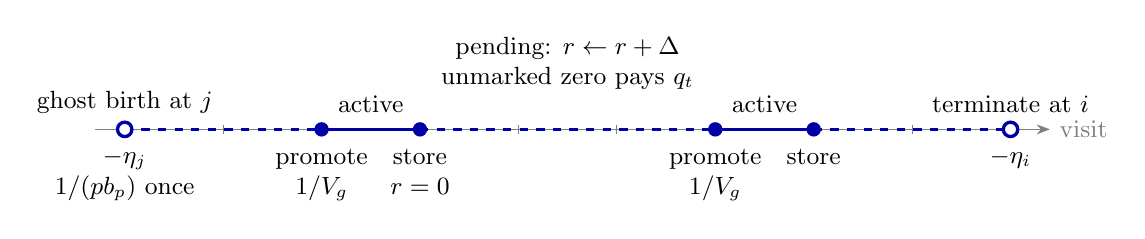
\begin{tikzpicture}[x=1.25cm,y=0.85cm,>=Stealth,
  every node/.style={font=\small}]
 \draw[->,gray] (-.3,0)--(9.4,0) node[right]{visit};
 \foreach \x in {0,...,9}{\draw[gray] (\x,-.07)--(\x,.07);}
 \draw[very thick,dashed,blue!65!black] (0,0)--(2,0);
 \draw[very thick,blue!65!black] (2,0)--(3,0);
 \draw[very thick,dashed,blue!65!black] (3,0)--(6,0);
 \draw[very thick,blue!65!black] (6,0)--(7,0);
 \draw[very thick,dashed,blue!65!black] (7,0)--(9,0);
 \foreach \x in {2,3,6,7}{\fill[blue!65!black] (\x,0) circle (2.6pt);}
 \foreach \x in {0,9}{\draw[draw=blue!65!black,fill=white,very thick]
    (\x,0) circle (2.6pt);}
 \node[above] at (0,.1){ghost birth at $j$};
 \node[above] at (2.5,.1){active};
 \node[above] at (6.5,.1){active};
 \node[above] at (9,.1){terminate at $i$};
 \node[below,align=center] at (0,-.15){$-\eta_j$\\$1/(pb_p)$ once};
 \node[below,align=center] at (2,-.15){promote\\$1/V_g$};
 \node[below,align=center] at (3,-.15){store\\$r=0$};
 \node[below,align=center] at (6,-.15){promote\\$1/V_g$};
 \node[below,align=center] at (7,-.15){store};
 \node[below] at (9,-.15){$-\eta_i$};
 \node[above,align=center] at (4.5,.45){pending: $r\gets r+\Delta$\\
                                  unmarked zero pays $q_t$};
\end{tikzpicture}
\caption{One possible lifespan.  Solid segments denote shared
activity; dashed segments denote memory.  Every marked use and
ghost endpoint has the same offset modulo $p$.  The reciprocal
prime factor is charged only at birth; $\eta_t=1-q_t$ at visit $t$.}
\label{fig:prime-lifespan}
\end{figure}

\subsection{Absolute bounds, including the adjoint measures}

The memory identity is exact with the global distinct-birth rule.
We now allow different births to have equal prime values, so that each
operation acts locally on $\mathcal H$.  We will restore the global rule
after estimating this enlarged evolution.  The absolute bounds proved
here justify the memory truncation and remain available when equality
constraints later modify individual operations.  Their column bounds
require the factorial adjoint measures explicitly.

For a positive row kernel $K$, if a positive function $w$ satisfies
$Kw\le Rw$ and $K^*w\le Cw$, then
\begin{equation}\label{eq:weighted-schur}
 \norm K_{2\to2}\le\sqrt{RC}.
\end{equation}
Indeed, Cauchy's inequality in each row bounds $|Kf|^2$ by
$(Kw)K(|f|^2/w)$; integration and the column inequality prove
\Cref{eq:weighted-schur}.  We apply this to absolute kernels,
with
\[
 w(\text{state})=v^{j_{\rm tot}},
 \qquad j_{\rm tot}=\sum_{g\in\mathcal B}j_g,
\]
where $v>1$ is a fixed constant chosen below.

Here is a direct verification of the measures in the ghost
adjoint.  In one group abbreviate
\[
 A_i=\frac{q_i}{\rho^2},\qquad
 D_i=-\frac{\eta_i}{\rho},\qquad C_i=V_gD_i,
 \qquad \nu=\widetilde\mu_g,
\]
and let $z(\mathbf u)$ count zero residues in a memory list.
For test functions $f,h$, the joint integral from
\Cref{eq:ghost-row} is
\begin{align}
 \langle f,G_{i,g}h\rangle
 ={}&\sum_{k,t,b\ge0}\frac1{k!t!b!}
 \int A_i^{z(\mathbf u)}D_i^tC_i^b
       \overline{f(\mathbf u,\boldsymbol\alpha^0)}
       h(\mathbf u,\boldsymbol\beta^0)\notag\\
 &\hspace{14mm}\cdot
 d\lambda_g^{\otimes k}(\mathbf u)
 d\nu^{\otimes t}(\boldsymbol\alpha)
 d\nu^{\otimes b}(\boldsymbol\beta).
 \label{eq:ghost-joint-integral}
\end{align}
Here $\boldsymbol\alpha^0$ means that all its residues are zero.
The identity follows by selecting $t$ old zero indices from
a list of size $k+t$:
\[
 \frac1{(k+t)!}\binom{k+t}{t}=\frac1{k!t!}.
\]
Swapping $(t,\boldsymbol\alpha)$ with
$(b,\boldsymbol\beta)$ and conjugating shows that the adjoint
has the same row formula with birth coefficient $D_i$ and
termination coefficient $C_i$.  In particular, reversal moves
the factor $V_g$ from births to terminations; it does not create
any factor $p$ or $1/p$.

For the absolute ghost kernel the weighted row ratio is exactly
\begin{equation}\label{eq:ghost-schur-ratios}
 \exp\bigl(|C_i|v\nu(\mathcal P_g)\bigr)
 \left(A_i+\frac{|D_i|}{v}\right)^{z(\mathbf z)},
\end{equation}
and its column ratio has $C_i,D_i$ interchanged.  Choose $v$
large enough that, for both possible $q_i$,
\begin{equation}\label{eq:memory-weight-choice}
 \frac{q_i}{\rho^2}+
 \frac{2\max(1,v_+)\eta_i}{\rho v}<1.
\end{equation}
This is possible since $q_i\le\sqrt q<\rho^2$.  The same
choice works when every original ghost birth receives an
extra factor two.  Since $\nu(\mathcal P_g)=1+o(1)$, the
exponential factor in \Cref{eq:ghost-schur-ratios} is bounded
by a fixed constant per group.  Thus for some fixed $C_v$,
\begin{equation}\label{eq:ghost-absolute-bound}
 |G_i|w\le L^{C_v}w,\qquad |G_i|^*w\le L^{C_v}w,
 \qquad \norm{G_i}\le L^{C_v}.
\end{equation}
The exponent $C_v$ is independent of $m,C_1,J$.  All these
assertions include the version with doubled ghost births.

We verify the edge adjoint just as explicitly.  Fix one big
group, a pattern, endpoint permutations, free labels, and
the chosen transfer subsets.  Suppose $a$ target slots are
promotions and $b$ source slots are stores, so $a,b\le t_g$.
Let the source memory have size $j$, and write $u$ for its
$j-a$ surviving particles.  Let $p_1,\ldots,p_a$ be the
promoted prime labels and $s_1,\ldots,s_b$ the stored labels.
For step $\Delta$, the endpoint memories are
\begin{equation}\label{eq:edge-joint-memory}
 X=u\sqcup((p_h,-\Delta\bmod p_h))_{h\le a},
 \qquad
 Y=T_\Delta u\sqcup((s_h,\Delta\bmod s_h))_{h\le b},
\end{equation}
where $T_\Delta$ translates every residue.  The joint measure
on these variables is
\begin{equation}\label{eq:edge-joint-measure}
 \frac{d\lambda_g^{\otimes(j-a)}(u)}{(j-a)!}
 \prod_{h\le a}d\widetilde\mu_g(p_h)
 \prod_{h\le b}d\widetilde\mu_g(s_h),
\end{equation}
along with one $\widetilde\mu_g$ integration for every shared
active label, dropped source label, and fresh target label.
The transfer coefficient is $V_g^{-a}$, and the damping is
$\rho^{z(X)+z(Y)}$.  The factorial accounting is
\begin{equation}\label{eq:edge-factorial-reversal}
 \frac{(j)_a}{j!}=\frac1{(j-a)!}
 =\frac{(j-a+b)_b}{(j-a+b)!}.
\end{equation}
The first equality selects old memory indices into the $a$
specified ordered target slots.  The second selects $b$
indices of the output memory into the original source slots
on reversal.  Each required residue in
\Cref{eq:edge-joint-memory} selects exactly one point of
counting measure.  Translation preserves that measure.

It follows that the reversed row operation retrieves the
original stores and stores the original promotions; the
coefficient $V_g^{-a}$ remains unchanged.  If it is expressed
using the forward convention that charges $V_g^{-b}$ for its
reversed promotions, its additional factor is $V_g^{b-a}$.
This is bounded uniformly for $a,b\le\ell+m$.  Fixing shared
and free $D$-labels fixes $\Delta$ independently of which
memory indices are retrieved, as required for this change
of variables.  In small groups Haar translation and the joint
normalization $V_g^{-M-\ell}$ are invariant on reversal.

The identities above continue to hold with numerical
coincidences.  For example, a memory multiset with multiplicities
$n_z$ has mass $\prod_z\lambda_g(z)^{n_z}/n_z!$.  Subset
deletions and ordered retrievals retain their index
multiplicities.  No passage from indices to distinct numerical
values was made in \Cref{eq:ghost-joint-integral} or
\Cref{eq:edge-factorial-reversal}.

\begin{lemma}[Absolute memory bounds]\label{lem:memory-absolute}
There is $C_a$, allowed to depend on $m,C_1$ but independent
of $J$, such that every absolute edge has weighted row and
column bounds $L^{C_a}$.  These bounds and
\Cref{eq:ghost-absolute-bound} persist under arbitrary
multipliers of modulus at most one on individual local
transition choices, and under memory-size projections.
\end{lemma}

\begin{proof}
For a row, fix a pattern, free labels, permutations, and
transfer-slot subsets of sizes $a_g,b_g\le t_g$.  If $Z'$
old pending particles have zero translated residue in a
group, their ordered promotions and the remaining output
damping cost at most
\begin{equation}\label{eq:promotion-count}
 (Z')_{a_g}\rho^{Z'-a_g}
 \le\sup_{z\ge a_g}(z)_{a_g}\rho^{z-a_g}<\infty.
\end{equation}
Damping of stored particles can be discarded for this upper
bound.  The Schur weight contributes $v^{b_g-a_g}$, promotion
coefficients contribute $V_g^{-a_g}$, and fresh integrations
have mass $\widetilde\mu_g(\mathcal P_g)^{t_g-a_g}\le2^{t_g}$
for large $x$.  There are at most $4^{t_g}$ choices of transfer
subsets.  Each cost is bounded by a constant per group,
independent of $J$.  Small transitions satisfy
\Cref{eq:physical-count-bound}.  Multiplying over groups,
averaging permutations and free labels, and summing
\Cref{eq:pattern-mass} proves the row bound.

For the column, use \Cref{eq:edge-joint-memory,eq:edge-factorial-reversal} in reverse.  Original stores
are now ordered retrievals.  Their count is controlled by the
original input $\rho$ factors after reversed translation, in
exactly the form in \Cref{eq:promotion-count}.  The remaining
factor $V_g^{b_g-a_g}$ is bounded per group.  This proves the
column bound.  Restrictions and local multipliers of modulus
at most one are dominated by these absolute kernels.
\end{proof}

We now restrict the total memory size to
\begin{equation}\label{eq:memory-truncation}
 B=\lceil L^2\rceil
\end{equation}
before and after every operation, writing the projections
implicitly.  At most $(\ell+m)|\mathcal B|N$ particles can
be supplied by stores.  Thus a path violating this restriction
has at least $B-O((\ell+m)sN)$ ghost births.  Multiply every
ghost birth by two in the absolute path sum and use the
preceding bounds.  The total omitted mass, even with the
distinct-birth indicator, is at most
\begin{equation}\label{eq:memory-tail}
 2^{-B+O((\ell+m)sN)}L^{O(N)}
 =\exp(-\Omega(L^2))=o(L^{-AN})
\end{equation}
for every fixed $A$.  The empty-memory boundary vector has
bounded norm: the small part has mass at most one by
\Cref{eq:initial-factorial-mass}, and the big part has mass
\[
 \prod_{g\in\mathcal B}
 \widetilde\mu_g(\mathcal P_g)^M
 =1+O_J(sN/P_*)=1+o(1).
\]
These estimates also prove absolute summability before
truncation, for instance by first restricting all batch sizes
and then applying monotone convergence to absolute kernels.

\subsection{Rare transfers and the role of the small groups}

It remains to obtain a small signed edge norm and then restore the
omitted distinct-birth rule.  Decompose each edge as
$\mathcal E_i=\mathcal E_{i,\rm clean}+\mathcal E_{i,\rm dirty}$:
a term is \emph{dirty} if it has at least one store or promotion, and
\emph{clean} otherwise.  Dirty terms connect memory to the active lists;
we suppress them by averaging the omitted small labels.  Clean terms
only translate memory residues and refresh unshared active labels; the
next subsection will reduce their norm to the ideal estimate.  Define
\begin{equation}\label{eq:small-omission-number}
 \mathcal D=\binom{M}{\ell}^{|\mathcal S|}.
\end{equation}

\begin{lemma}[Rare transfer]\label{lem:rare-transfer}
With the memory truncation in \Cref{eq:memory-truncation}, the
aggregate of all dirty terms of any edge has norm at most
\begin{equation}\label{eq:dirty-norm}
 2L^{C_a}\left(\frac B{\mathcal D}\right)^{1/2},
\end{equation}
after enlarging $C_a$ independently of $J$ if necessary.
\end{lemma}

\begin{proof}
First consider the positive sum of terms with a promotion.
Fix its source, pattern, big-group permutations and shared
choices, and free $D$-labels.  For some one of its at most
$B$ old pending particles $(p,r)$, promotion requires
\begin{equation}\label{eq:promotion-congruence}
 r+\sigma_i kD_{\mathcal B}D_{\mathcal S}\equiv0\pmod p,
 \qquad p\nmid D.
\end{equation}
In each small group the source symmetrization omits an
independent uniformly chosen $\ell$-subset of its $M$
distinct labels.  If $F$ is the full product of all small
source labels and $U$ the product of the omitted labels,
then $D_{\mathcal S}=F/U$.  Unique factorization and
disjointness of groups show that the $\mathcal D$ choices
give distinct positive integers $U$.  Moreover,
\[
 U\le\exp(\ell|\mathcal S|L^b)<\exp(L^c)\le p
\]
for sufficiently large $x$.  They are therefore distinct
modulo $p$.  The quantities $F,k,D_{\mathcal B}$ are
invertible modulo every $p$ eligible in
\Cref{eq:promotion-congruence}.  Hence each pending particle
allows at most one omission choice.  At most $B$ of the
$\mathcal D$ equally likely choices allow any promotion.

Conditional on every omission choice, the remaining weighted
row costs are uniformly bounded by the proof of
\Cref{lem:memory-absolute}.  Thus the promotion part improves
its row bound to $L^{C_a}B/\mathcal D$, while its column
bound remains $L^{C_a}$.  Schur's test gives the first half
of \Cref{eq:dirty-norm}.  Terms with stores and no promotion
have the same improvement in their column bound by reversing
the edge: a stored particle becomes a retrieval from output
memory.  The exclusion $p\nmid D$ is retained under reversal,
even when numerical coincidences have been allowed.  Add
these two bounds.
\end{proof}

The coefficient restriction to big labels is used here:
conditioning on all such labels does not bias the small
omission choices.  In particular,
\begin{equation}\label{eq:dirty-J-gain}
 2L^{C_a}\sqrt{B/\mathcal D}
 \ll L^{C_a+1-(c_0/2)\log\binom{J+\ell}{\ell}}.
\end{equation}
An arbitrarily strong fixed saving is obtained by increasing
$J$, without changing the ideal norm target.

\subsection{Clean edges and Fourier reduction}

\begin{lemma}[Clean norm]\label{lem:clean-norm}
There is $C_s$, depending only on the fixed data in
\Cref{def:prime-groups}, such that the clean part of every
edge satisfies
\begin{equation}\label{eq:clean-norm}
 \norm{\mathcal E_{i,\rm clean}}
 \le 2L^{-E_{\rm id}+C_s}
\end{equation}
for all sufficiently large $x$, under
\Cref{eq:ideal-norm-hypothesis}.  In particular $C_s$ is
independent of $m,C_1,J$.
\end{lemma}

\begin{proof}
A clean edge leaves all memory prime lists and sizes
unchanged, translates their residues, drops every unshared
big source slot, and fills every unshared big target slot
freshly.  Its input and output $\rho$ factors and its
memory projections are contractions.  They commute with
active-list symmetrizations.  Absorb these factors and the
symmetrizations into the two test vectors $w_1,w_2$.
These vectors remain symmetric in the big active lists.

Fix an ordered tuple $\mathbf d$ of $J$ shared labels in
each small group and let $d'$ denote their joint product.
Define a map to unrestricted small residue functions by
\begin{equation}\label{eq:small-conditioning-map}
 (P_{\mathbf d}w)(y)=
 \left(\prod_{g\in\mathcal S}V_g^{-J/2-\ell}\right)
 q^{\frac12\sum_{g\in\mathcal S}(\omega_g(y)-M)}
 \sum_{\mathbf R:\ (\mathbf d,\mathbf R)\text{ a small state at }y}
             w(y,(\mathbf d,\mathbf R)).
\end{equation}
All other coordinates are left untouched.  The map is zero
when the displayed list is not a small state, so the damping
is used only where $\omega_g(y)\ge M$.  The two endpoint
factors in \Cref{eq:small-conditioning-map} give
$V_g^{-J-2\ell}=V_g^{-M-\ell}$, exactly the physical joint
normalization.

By Cauchy's inequality in $\mathbf R$, followed by summation
over $\mathbf d$, one has
\begin{equation}\label{eq:small-map-norm}
 \sum_{\mathbf d}\norm{P_{\mathbf d}w}^2
 \le L^{C_s}\norm w^2.
\end{equation}
To see the independence of $J$, the multiplier relative to
the original small state measure in group $g$ is bounded by
\[
 \sup_{z\ge M}
 q^{z-M}\frac{(z-M+\ell)_\ell}{V_g^\ell},
\]
a constant depending only on $q,\ell,v_-$.  Taking products
over $O(T)$ groups proves \Cref{eq:small-map-norm}.

The clean bilinear form is now exactly
\begin{equation}\label{eq:clean-conditioned-form}
 \sum_{\mathbf d}
 \langle P_{\mathbf d}w_1,
                \mathcal T'_{\mathbf d}P_{\mathbf d}w_2\rangle.
\end{equation}
The operator between these maps uses the big-list transitions
and translates all unrestricted small and memory residues
by $\sigma_i kd'D_{\mathcal B}$.  Fix the memory sizes and
their prime lists.  Fourier transformation on the finite
abelian group consisting of the small residue torus and
the pending residue coordinates diagonalizes these
translations.  Counting measure on pending residues and
Haar measure on the small torus each have the usual unitary
finite Fourier transform.  One can first use ordered memory
representatives; restriction to symmetric functions preserves
the bound.  Big active-list symmetry is unaffected.

At any fixed Fourier frequency, translation and the closure
factor contribute
\[
 \ee{\sigma_i\Theta D_{\mathcal B}}
\]
for a real $\Theta$ depending on $\mathbf d$, the memory
prime list, the frequency, and $\theta$, but independent
of the variable big active labels.  The scalar factor
$(d')^{\sigma_i i\zeta}$ has modulus one.  Consequently
the remaining operator, on symmetric big active tests, is
$\mathcal T(\Theta)$ or its adjoint, with two changes only:
the measures of active labels and fresh target integrations
are $\widetilde\mu_g$ in place of $\mu_g$, and the
free/active collision ban remains in force.

Both changes are negligible in operator norm.  Across the
$M|\mathcal B|$ active coordinates, the product density
changes by
\[
 1+O_J(sN/P_*).
\]
The corresponding square-root density identification is
unitary between the two $L^2$ spaces and commutes with
symmetrization.  Fresh integration densities obey the
same bound.  The ideal absolute row and column sums are
at most $L^{C_1}$ before these changes, since all its
unrestricted fresh laws are probabilities.  Schur's test
therefore bounds the density perturbation by
$O_J(L^{C_1}sN/P_*)$.

For the ban, in either row direction condition on the
fixed active state.  Each free auxiliary draw has maximal
atom $O(1/P_*)$; its chance to match a fixed active label
is bounded by that quantity.  A match to a fresh opposite
unshared label has the same bound by independence.
There are $O_{J,m}(s)$ possible comparisons.  Reversal
has the same estimate.  Thus removing the banned
transitions costs $O_{J,m}(L^{C_1}s/P_*)$ in norm.
These estimates are $o(L^{-A})$ for every fixed $A$.
They do not require exclusion of coincidences with
pending labels: such labels are fixed in the Fourier
decomposition and are already accounted for by translation.

It follows uniformly in $\mathbf d$ that the between-map
norm is at most $2L^{-E_{\rm id}}$ for large $x$.  Apply
Cauchy's inequality to \Cref{eq:clean-conditioned-form}
and then \Cref{eq:small-map-norm}; this proves
\Cref{eq:clean-norm}.
\end{proof}

Choose, in this order,
\begin{equation}\label{eq:transference-parameter-choice}
 G>E+C_v+3,\qquad E_{\rm id}>G+C_s+2,
\end{equation}
and finally choose the fixed integer $J$ so large that
\Cref{eq:dirty-J-gain} is smaller than
$\tfrac12L^{-G}$ for large $x$.  For example it suffices
that
\[
 \frac{c_0}{2}\log\binom{J+\ell}{\ell}>C_a+G+3.
\]
The clean estimate supplies the other half.  Hence the
whole signed truncated edge, with birth distinctness
still omitted, satisfies
\begin{equation}\label{eq:whole-edge-contraction}
 \norm{\mathcal E_i}\le L^{-G}.
\end{equation}
Only this final choice of $J$ needs to depend on $m,C_1$.
This establishes the required quantifier order, but a
further argument is necessary to impose distinct births
without losing the signed contraction on every edge.

\subsection{Restoring distinct births by equality rank}

A single absolute collision estimate cannot finish the proof: one
reciprocal-prime saving $P_*^{-1}$ does not absorb a length-$N$ absolute
path cost $L^{O(N)}$.  Instead, expand the global distinctness condition
by equalities between birth values.  Many independent equalities yield
many point-mass savings.  A small number of independent equalities can
be imposed by phases at their birth operations, preserving the signed
contraction on all the other edges.

In the truncated evolution allocate potential birth
addresses as follows: initial big slots; every possible
big target slot at every edge, in its canonical order
before final symmetrization; and indices $1,\ldots,B$
in each group's ordered ghost batch at each visit.
A target slot is performed as an address precisely when
it is a fresh birth rather than shared or promoted.
A ghost address is performed precisely when its batch
is at least that large.  These are conditions on the
choices made in their single local operation.  The
number $A_*$ of potential addresses satisfies
\begin{equation}\label{eq:birth-address-count}
 A_*\le M|\mathcal B|(N+1)+(N+1)|\mathcal B|B=L^{O(1)}.
\end{equation}
The implied exponent can be taken independent of $J$
once $x$ is sufficiently large for fixed $J$.

We use the following elementary form of distinctness
inclusion-exclusion.  Sum over collections $\pi$ of
disjoint blocks of potential addresses, every block
having size at least two.  Let $\mathcal C_\pi$ require
that all addresses in those blocks be performed and
that the prime values within each block be equal.  Set
\begin{equation}\label{eq:distinct-birth-expansion}
 \mu(\pi)=\prod_{B'\in\pi}(-1)^{|B'|-1}(|B'|-1)!,
 \qquad r(\pi)=\sum_{B'\in\pi}(|B'|-1).
\end{equation}
For a fixed realized path,
\begin{equation}\label{eq:distinct-indicator}
 \ind_{\text{distinct performed birth values}}
       =\sum_\pi\mu(\pi)\ind_{\mathcal C_\pi}.
\end{equation}
To verify this, interpret a block of size $h$ as a cycle
on its $h$ addresses: there are $(h-1)!$ such cycles,
each with sign $(-1)^{h-1}$.  The right side is the sum
of signs of permutations of the performed addresses
which preserve their numerical prime values.  It factors
over equal-value classes.  The sign sum is one for a
singleton class and zero for any class of size at least
two, by pairing permutations with their product by a
fixed transposition.

A rank-$r$ collection involves at most $2r$ addresses.
More precisely its total absolute coefficient, summed
over all collections of rank $r$, obeys
\begin{equation}\label{eq:rank-coefficient-count}
 \sum_{r(\pi)=r}|\mu(\pi)|\le A_*^{2r}\le L^{C'r}.
\end{equation}
For instance the unsigned cycle generating polynomial
on $A_*$ addresses is $\prod_{j=0}^{A_*-1}(1+jt)$,
where the power of $t$ is the sum of cycle lengths
minus the number of cycles.  Its coefficient of $t^r$
is at most $(\sum_jj)^r/r!\le A_*^{2r}$.

\paragraph{Large rank: chronological fresh integrations.}
Fix $\pi$.  Order birth addresses chronologically, using
canonical slot order inside an edge or batch, and call
the first address in each block its pivot.  Every other
address is a dependent birth.  When such an address is
performed, its fresh prime integration is constrained
to the already determined pivot value.  Since
\begin{equation}\label{eq:tilted-point-mass}
 \sup_{g\in\mathcal B,p\in\mathcal P_g}
                 \widetilde\mu_g(p)\ll P_*^{-1},
\end{equation}
this improves the weighted absolute row bound by
$O(P_*^{-1})$ per dependent birth.

Here the chronological assertion uses genuinely fresh
integrations.  At an edge choose stores, promotions,
and the step first, and then fill fresh target slots in
canonical order.  The step, promotion count, and memory
weight do not depend on these new prime values; the
coefficient is bounded by its supremum and exclusions
may be discarded.  In the proof of
\Cref{lem:memory-absolute}, replace the total fresh mass
in each constrained slot by its single-point bound.
For a ghost operation keep its ordered batch integral
and factorial divisor; constraining indicated fresh
coordinates replaces their mass factors by the same
single-point bound.  The birth coefficient $V_g$ and
the memory weight only give fixed constants per
constrained coordinate.  Initial active slots satisfy
the same product estimate.  Pivots and dependents
within one operation are handled in their prescribed
integration order.

For completeness, these conditional row bounds can be
iterated although a pivot may have died before its
dependent birth.  Retain all pivot values in the
conditioning.  Bound the remaining terminal sum by
backward induction using the uniform weighted row
bounds for every possible conditioning, beginning
with $\mathbf1_\varnothing\le w$.  Whenever a dependent
birth is reached, the preceding point-mass improvement
is uniform in its retained pivot value.  At the initial
boundary $w=1$, and the remaining integrated boundary
mass is bounded.  Thus the total absolute contribution
for this fixed collection is at most
\begin{equation}\label{eq:high-rank-path-bound}
 L^{C_h(N+1)}(C/P_*)^{r(\pi)},
\end{equation}
for fixed $C_h,C$; both may depend on $m,C_1$.

Choose a sufficiently large fixed $C''$, after these
constants and $C'$, and set
\begin{equation}\label{eq:rank-threshold}
 r_0=\left\lceil\frac{C''NT}{\log P_*}\right\rceil.
\end{equation}
By \Cref{eq:rank-coefficient-count} and
\Cref{eq:high-rank-path-bound}, the sum over $r\ge r_0$
is bounded by
\[
 L^{C_h(N+1)}\sum_{r\ge r_0}
               (CL^{C'}/P_*)^r=o(L^{-EN}).
\]
Indeed $\log P_*=L^c\gg T$, and increasing $C''$
beats the fixed exponent $C_h+E$.

\paragraph{Small rank: phases only at the affected births.}
For a block with pivot $\beta_0$ and other addresses
$\beta_1,\ldots,\beta_{h-1}$, equality of the integer
prime values has the exact representation
\begin{equation}\label{eq:birth-equality-fourier}
 \ind_{p_{\beta_j}=p_{\beta_0}\ (1\le j<h)}
 =\int_{[0,1]^{h-1}}
 \ee{\sum_{j=1}^{h-1}\tau_j(p_{\beta_j}-p_{\beta_0})}
             \,d\boldsymbol\tau,
\end{equation}
on paths performing all these addresses.  For fixed
Fourier parameters, collect the factors by their birth
operation.  Each affected operation is multiplied,
on its individual local choices, by
\[
 \ind_{\text{designated local births are performed}}
       \ee{\sum_{\beta\ \text{local}}c_\beta p_\beta},
\]
of modulus at most one.  Initial-slot factors merely
modify the initial boundary vector by such a multiplier.
An affected edge can lose its signed norm saving, but
\Cref{lem:memory-absolute} bounds its new norm by
$L^{C_a}$.  Unaffected edges retain their complete signed
pattern sum and both symmetrizations, so
\Cref{eq:whole-edge-contraction} still applies.

The ordered indices in a ghost batch do not require
ordered-memory functions.  For a batch of size $b$, insert
its local multiplier $\phi_b(p_1,\ldots,p_b)$ inside
the existing $1/b!$ product integral in
\Cref{eq:ghost-row}.  The rest of that integral is
symmetric in its fresh variables, so its value is
unchanged on replacing $\phi_b$ by
\[
 \frac1{b!}\sum_{\sigma\in S_b}
       \phi_b(p_{\sigma(1)},\ldots,p_{\sigma(b)}).
\]
This average has modulus at most one, also on numerical
diagonals.  The resulting operator acts on symmetric
memories, and its reversed multiplier is the conjugate
on the corresponding deleted batch in
\Cref{eq:ghost-joint-integral}.  Its absolute row and
column bounds remain \Cref{eq:ghost-absolute-bound}.
In particular no phase has to follow a particle through
later storage, propagation, or promotion: equality was
encoded entirely at its two birth addresses.

At most $2r$ edges are affected by a rank-$r$ collection.
The boundary norms are bounded, and all $N+1$ ghost
operations cost at most $L^{C_v}$.  Therefore its
Fourier-integrated contribution is at most
\begin{equation}\label{eq:low-rank-path-bound}
 O\left(L^{(-G+C_v)N+C_v+2r(G+C_a)}\right).
\end{equation}
Since
\[
 \frac{r_0}{N}=O(T/L^c)+O(N^{-1})=o(1),
\]
the sum over $r<r_0$, with the coefficient bound
\Cref{eq:rank-coefficient-count}, is
\[
 L^{(-G+C_v+o(1))N}=o(L^{-EN})
\]
by \Cref{eq:transference-parameter-choice}.

Thus the high-rank terms are controlled by their fresh-label costs,
while the low-rank terms retain signed contraction on $N-o(N)$ edges.
Together they bound the expansion with distinct births, which is the
expression required by \Cref{lem:memory-identity}.

\begin{proof}[Completion of \Cref{thm:transference}]
Apply \Cref{eq:distinct-indicator} in the truncated
memory identity.  The large- and small-rank estimates
bound it by $o(L^{-EN})$, uniformly in $\theta$.
Restore the tail \Cref{eq:memory-tail}; multiply by
the baseline, which is at most one; and integrate
\Cref{eq:return-fourier}.  Finally restore the
uniform residue-replacement error, choosing its
precision after the absolute path bound.  The result
is $o(L^{-EN})$, and therefore
\Cref{eq:transference-moment} for sufficiently large
$x$.  The choice of $E_{\rm id}$ in
\Cref{eq:transference-parameter-choice} depends only
on $E,C_v,C_s$, and the dependence of these constants
was stated above.  This completes the proof with
the asserted quantifiers.
\end{proof}

\subsection{The endpoint pairing consequence}

We now convert the root moment into the pairing estimate used in
\Cref{sec:shifts}.  Constancy on a mark fiber is needed only at the first
endpoint; the second endpoint can be any vector with the stated norm.

\begin{corollary}\label{cor:transference-pairing}
Under the hypotheses and choices of
\Cref{thm:transference}, let $f\in\mathcal H_{\rm ph}$
be supported on positions $I=[X,2X)$ and independent
of the chosen marks, with value $f_n$ at position $n$.
Suppose
\[
 \sup_{n\in I}|f_n|\le\exp(O(\sqrt L)),\qquad
 \norm f,\norm g\le X^{1/2}L^{C_3}.
\]
Then
\begin{equation}\label{eq:transference-pairing}
 |\langle f,\mathcal A g\rangle|
       \ll XL^{-E+2C_3}.
\end{equation}
Only the first endpoint must be independent of its
mark list.
\end{corollary}

\begin{proof}
Let $H\ge1$ bound every displacement $|kD|$.  Since
$D$ has $Js$ factors, all at most $\exp(L^d)$,
\begin{equation}\label{eq:maximum-graph-step}
 \log H=O_J(TL^d).
\end{equation}
Partition $I$ into consecutive intervals $I_j$ of
length $\lceil H\rceil$, except possibly the last.
Put $f_j=\ind_{I_j}f$ and restrict $g$ to the
$H$-neighborhood of $I_j$ to obtain $g_j$.  These
neighborhoods have bounded overlap, and
\[
 \langle f,\mathcal A g\rangle
       =\sum_j\langle f_j,\mathcal A g_j\rangle,
 \qquad \sum_j\norm{g_j}^2\ll\norm g^2.
\]
For $B_0=\mathcal A\mathcal A^*\ge0$, spectral
H\"older gives
\[
 |\langle f_j,\mathcal A g_j\rangle|
 \le\norm{g_j}\norm{f_j}^{1-1/R}
       \langle f_j,B_0^Rf_j\rangle^{1/(2R)}.
\]
The finite matrix
$(\langle u_n,B_0^Ru_m\rangle)_{n,m\in I_j\cap\Z}$
is positive semidefinite.  Its largest eigenvalue is
at most its trace, so mark independence implies
\[
 \langle f_j,B_0^Rf_j\rangle
 \le\left(\sum_{n\in I_j\cap\Z}|f_n|^2\right)d_j,
 \qquad
 d_j:=\sum_{n\in I_j\cap\Z}
                  \langle u_n,B_0^Ru_n\rangle.
\]
There is no assertion here that the $u_n$ have equal
norm, or that ordered lists return to their starting
values.  By \Cref{eq:maximum-graph-step},
\[
 \left(O(H)\sup|f_n|^2\right)^{1/(2R)}
 =\exp\left(O_J\left(\frac{TL^d+\sqrt L}{L^{0.52}}\right)\right)
 =O(1).
\]
Sum the resulting block bounds by H\"older with
exponents $2$, $2R/(R-1)$, and $2R$.  This gives
\[
 |\langle f,\mathcal A g\rangle|
 \ll\norm g\,\norm f^{1-1/R}
                       \left(\sum_jd_j\right)^{1/(2R)}.
\]
The theorem bounds the last sum by
$|I\cap\Z|L^{-2RE}\ll XL^{-2RE}$.
Substitution of the two endpoint norm bounds proves
\Cref{eq:transference-pairing}; the extra factor
$L^{-C_3/R}$ is bounded for fixed $C_3$.
\end{proof}

\section{Small ideal kernels at every frequency}\label{sec:ideal}

We use the groups and probability measures of \Cref{sec:transference}.
In this section each big group $\mathcal P_g$, $g\in\mathcal B$, is
the set of primes in an interval contained in
$[\exp(L^c),\exp(L^d)]$.  In particular, intersecting a group with a
further interval again gives an interval of primes.  This additional
assumption allows us to use \Cref{thm:sw} with one label varying and all
other labels fixed.

\begin{theorem}[Construction of the residual ideal operator]
\label{thm:ideal}
Fix $E_{\rm id}>0$ and a fixed frequency exponent $C_4\geq0$.
There are fixed integers $m,J_0$ and a fixed constant $C_1$, depending
only on these parameters, $\ell$, and the prime-group bounds, with the
following property.  For every fixed $J\geq J_0$, there is a family
consisting of the raw pattern
\[
 C_g=\varnothing\quad\hbox{for every }g,\qquad K_0=1,
\]
and signed comparison patterns satisfying
\[
 C_g=\varnothing\ (g\in\mathcal S),\qquad
 |C_g|\leq m\ (g\in\mathcal B),\qquad
 \sum_\nu\sup|K_\nu|\leq L^{C_1},
\]
such that the symmetrized ideal operator of \Cref{sec:transference}
satisfies
\begin{equation}\label{eq:ideal-small-norm}
 \sup_{\Theta\in\R,\ |\zeta|\leq L^{C_4}}
 \norm{\mathcal T(\Theta)}_{2\to2}\leq L^{-E_{\rm id}}
\end{equation}
for sufficiently large $x$.  The coefficients and the family are
independent of $\Theta$ and of the individual value of $\zeta$.
Their defining parameters are independent of $J$; $J$ only supplies
the available shared slots.  The threshold for $x$ may depend on $J$.

More precisely, designate $m$ of the first $J$ slots in each big group
as probes, and split the big groups into two blocks. Each comparison
frees nonempty sets $A$ and $B$ of designated probes in the respective
blocks, and its coefficient has the form
\begin{equation}\label{eq:ideal-comparison-coefficient}
 -(-1)^{|A|+|B|}\mathcal K_A(D_A,X_A)
                         \mathcal K_B(D_B,X_B).
\end{equation}
Here $D_A,D_B$ are the products of the free labels used to form $D$,
$X_A$ is the product of the target labels in $A$, and $X_B$ the
product of the input labels in $B$.  These coefficients use no
shared labels and none of the last $\ell$ labels.  Each kernel is
a finite sum of products of matched log-cell indicators and pairs of
Dirichlet characters of conductor bounded by a fixed power of $L$.
\end{theorem}

The construction separates an approximation from a cancellation. We first
build kernels that replace selected shared products by independent products
in a bilinear pairing, for each prescribed fixed error exponent. The tests may depend on the entire ordered label tuples, as they
will when we condition on the labels outside the freed slots.

The cancellation then decomposes the input test in the first-block probes
and the target test in the second-block probes. Each decomposition is
orthogonal: its pieces are mean zero in a specified set of these probe
coordinates and independent of the others. Freeing $A$ averages the
source coordinates in $A$, and freeing $B$ averages the target coordinates
in $B$; the asymmetric coefficient above leaves these coordinates absent
from the multiplier. Thus only components independent of the freed
coordinates survive. Alternating subset signs cancel every pair for which the input component
is independent of at least one first-block probe and the target component
is independent of at least one second-block probe.
Every remaining pair contains a component that is mean zero in every
probe of one block. Such components have small norms by permutation
symmetry and the averaging of the last $\ell$ coordinates. We prove this cancellation after the
comparison estimate, so that its use on conditional tuple tests is explicit.

All label tuples in the next three subsections have their product
probability measure, with repetitions allowed.

\subsection{Products of labels and an elementary bilinear bound}

Let $\Lambda$ be a nonempty set of slots, using $k_g\leq m$ slots
from group $g$, and let $P_\Lambda$ denote the product of its labels.
Disjointness of the prime groups and unique factorization give, on
the support of this product,
\begin{equation}\label{eq:ideal-product-atom}
\begin{gathered}
 \rho_\Lambda(n):=\Prob(P_\Lambda=n)
 =\frac1n\prod_g
     \frac{k_g!}{V_g^{k_g}\prod_{p\in\mathcal P_g}a_p!}
 \leq\frac{L^\kappa}{n},\\
 \kappa=C_0\bigl(\log(m!)+m\log\max(1,v_-^{-1})\bigr),
\end{gathered}
\end{equation}
where $a_p$ is the multiplicity of $p$ in $n$.  The probability is
zero if the prescribed group multiplicities do not hold.  Indeed,
each factor apart from $1/n$ is at most
$m!\max(1,v_-^{-1})^m$, and there are at most $C_0T$ big groups.
In particular, this exponent does not depend on $J$.

This estimate applies to tests on the entire ordered label tuple.
If $f$ is any such $L^2$ test, supported where $c_1U\leq
P_\Lambda\leq c_2U$ for fixed $c_1,c_2>0$, put
$a_n=\E[f\ind_{P_\Lambda=n}]$.  Cauchy--Schwarz on each fiber gives
\begin{equation}\label{eq:ideal-collapse}
 \sum_n|a_n|^2
 \leq\sum_n\rho_\Lambda(n)
                 \E[|f|^2\ind_{P_\Lambda=n}]
 \leq\frac{L^\kappa}{c_1U}\norm f_2^2.
\end{equation}
No assumption that $f$ is a function of the product has been made.

\begin{lemma}[Integer bilinear estimate]\label{lem:bilinear}
Let $U,V\geq1$.  Suppose $a_n,b_t$ are supported in integer
intervals of lengths at most $C U,C V$, respectively, where $C$ is
fixed.  If
\[
 \alpha=u/r+\beta,\qquad (u,r)=1,\quad r\geq1,
 \qquad |\beta|\leq r^{-2},
\]
then
\begin{equation}\label{eq:integer-bilinear}
 \left|\sum_{n,t}a_nb_t\ee{\alpha nt}\right|
 \ll_C \norm a_{\ell^2}\norm b_{\ell^2}
 \left[U+(1+V/r)\{U+r\log(2r)\}\right]^{1/2}.
\end{equation}
The containing intervals need not begin at $1$, and the
coefficients may vanish on arbitrary subsets of them.
\end{lemma}

\begin{proof}
Extend the coefficients by zero to their containing intervals.
Cauchy--Schwarz in $n$, followed by expansion of the square and
the geometric-sum bound on the full interval of $n$, gives
\begin{align*}
 \left|\sum_{n,t}a_nb_t\ee{\alpha nt}\right|^2
 &\ll_C\norm a_{\ell^2}^2
 \left(U\sum_t|b_t|^2+
   \sum_{1\leq |h|\leq CV}
    \min\{U,\norm{\alpha h}_{\R/\Z}^{-1}\}
       \sum_t|b_t b_{t+h}|\right)\\
 &\ll_C\norm a_{\ell^2}^2\norm b_{\ell^2}^2
  \left(U+\sum_{1\leq h\leq CV}
         \min\{U,\norm{\alpha h}_{\R/\Z}^{-1}\}\right).
\end{align*}
At a zero denominator the minimum is interpreted as $U$.
For $r\geq2$, split the $h$-range into
$O_C(1+V/r)$ consecutive blocks, each of diameter at most $r/2$.
If $h\ne h'$ belong to a block, their difference is nonzero and
has magnitude less than $r$, so
\[
 \norm{\alpha(h-h')}_{\R/\Z}
 \geq\norm{u(h-h')/r}_{\R/\Z}
            -\frac{|h-h'|}{r^2}\geq\frac1{2r}.
\]
Thus the phases in a block are $1/(2r)$-separated on the circle.
Ordering them by distance from zero bounds their contribution by
\[
 O_C\left(U+\sum_{1\leq j\leq 2r}\frac rj\right)
 =O_C\bigl(U+r\log(2r)\bigr).
\]
For $r=1$, the trivial bound $O_C(UV)$ for the whole sum gives
the asserted estimate.  This proves the lemma.
\end{proof}

For two independent selected products of sizes $U,V$, combining
\Cref{eq:ideal-collapse,eq:integer-bilinear} shows that the
probability-space bilinear form with phase $\ee{\alpha P_A P_B}$
has norm at most
\begin{equation}\label{eq:ideal-probability-bilinear}
 C L^\kappa
 \left(\frac1V+\frac1r+\frac{\log(2r)}U+
                   \frac{r\log(2r)}{UV}\right)^{1/2}.
\end{equation}
The same assertion holds with the phase multiplied by
$(P_AP_B)^{i\zeta}$ for any real $\zeta$, since this factor
separates between the two tests and preserves their norms.

\subsection{Log cells and conditional character operators}

For a fixed nonempty slot set $\Lambda$, let $D,X$ be independent
products of label tuples of this type.  Given $Q\geq1$, $0<h\leq1$,
and $0<\xi\leq1$, put
\[
 I_j=[jh,(j+1)h),\qquad
 \nu_{\Lambda j}=\Prob(\log D\in I_j),\qquad
 \mathcal C_Q=\{\chi:\chi\text{ primitive},\ \operatorname{cond}\chi\leq Q\}.
\]
The conductor-$1$ character is included.  Define
\begin{equation}\label{eq:ideal-cell-kernel}
 \mathcal K_\Lambda(D,X)
 =\sum_{j:\nu_{\Lambda j}\geq\xi}
   \frac{\ind_{\log D\in I_j}\ind_{\log X\in I_j}}{\nu_{\Lambda j}}
        \sum_{\chi\in\mathcal C_Q}\overline{\chi(D)}\chi(X).
\end{equation}
We use $\mathcal K_A,\mathcal K_B$ for the corresponding slot sets.
All powers of $L$ chosen below are fixed before $J$.

There are at most $Q^2$ characters in $\mathcal C_Q$.  The number
$N_\Lambda$ of cells of positive mass satisfies
\begin{equation}\label{eq:ideal-cell-costs}
 N_\Lambda\ll_m1+T L^d/h,\qquad
 \sup|\mathcal K_\Lambda|\leq Q^2\xi^{-1},\qquad
 \sup_X\E_D|\mathcal K_\Lambda(D,X)|\leq Q^2.
\end{equation}
The last inequality follows because, for fixed retained $X$,
the mass $\nu_{\Lambda j}$ of its cell cancels the denominator.
The kernel is zero for discarded $X$ and has support only where
$|\log D-\log X|<h$.

We record explicitly the character estimate under a cell
restriction.  If $Q$ is a fixed power of $L$ and $\chi,\chi'$ are
distinct members of $\mathcal C_Q$, then, for every fixed $D_*>0$,
\begin{equation}\label{eq:ideal-character-cell}
 \left|\E\left[\ind_{\log D\in I_j}
          \overline{\chi(D)}\chi'(D)\right]\right|
 \ll_{D_*}L^{-D_*},
\end{equation}
uniformly in $j$ and in the nonempty slot set with at most $m$
slots per group.  To see this, hold all but one label fixed.
The cell and the selected prime group restrict the remaining
prime to an interval, possibly empty.  The character
$\overline\chi\chi'$ on the common modulus is nonprincipal:
otherwise the uniqueness of primitive induction would imply
$\chi=\chi'$.  Its modulus is at most $Q^2$.  For every fixed $K$,
 \Cref{thm:sw}, summed against the character over reduced
residue classes and applied with a larger accuracy exponent, gives
\[
 A_\rho(t):=\sum_{p\leq t}\rho(p)
       \ll_K t(\log t)^{-K}
\]
for these nonprincipal characters, uniformly for
$t\geq y:=\exp(L^c)$.  The allowed modulus is a fixed power of
$\log y$, as required there.  Partial summation on any subinterval
of $[y,\exp(L^d)]$ bounds its reciprocal-prime sum by
\[
 O_K\left((\log y)^{-K}+
            \int_y^\infty\frac{dt}{t(\log t)^K}\right)
 =O_K\bigl((\log y)^{1-K}\bigr).
\]
Divide by $V_g\geq v_-$ and choose $K$ sufficiently large in terms
of $D_*$.  Averaging the other labels proves
\Cref{eq:ideal-character-cell}; its precision is independent of
the width or location of the interval.

For a retained cell of mass $\nu$, the integral operator defined
by \Cref{eq:ideal-cell-kernel} is the character frame operator on
the conditional probability space:
\begin{equation}\label{eq:ideal-frame}
 f\longmapsto\sum_{\chi\in\mathcal C_Q}
       \chi\,\langle\chi,f\rangle_{L^2(\Prob(\cdot\mid I_j))}.
\end{equation}
Its nonzero eigenvalues are those of the character Gram matrix.
Every diagonal entry is $1$, since all selected primes exceed
$Q^2$ for large $x$.  By \Cref{eq:ideal-character-cell}, every
off-diagonal entry is $O_{D_*}(\xi^{-1}L^{-D_*})$.
The Gram matrix therefore has norm at most
\begin{equation}\label{eq:ideal-gram-bound}
 1+O_{D_*}(Q^2\xi^{-1}L^{-D_*})\leq2
\end{equation}
once the character precision has been chosen sufficiently large.
Passing from the conditional to the original measure multiplies
both squared norms by $\nu$, so the operator norm is unchanged.
Different cells are orthogonal blocks, and discarded cells have
zero operator.  Consequently kernel integration on the full
label space has norm at most $2$.  The adjoint and transpose have
the same bound, so the integration may be moved onto either test
in a bilinear form.  In particular neither a cell-count factor
nor a factor $\xi^{-1}$ is lost in this operator norm.

\subsection{Uniform comparison for arbitrary tuple tests}

\begin{lemma}[Comparison kernel]\label{lem:comparison-kernel}
Fix $m$, $A_0>0$, and $C_4\geq0$.  There are fixed powers
$Q,h^{-1},\xi^{-1}$ of $L$, independent of $J$, such that the
kernels in \Cref{eq:ideal-cell-kernel} have the following property.
Let $A,B$ be nonempty sets of slots, using at most $m$ slots per
big group.  Take independent label tuples for
$D_A,X_A,D_B,X_B$ with the prescribed slot laws.  If $f$ and $g$
are arbitrary $L^2$ tests on the tuples making up $X_B$ and
$X_A$, respectively, then for every $\alpha\in\R$ and
$|\zeta|\leq L^{C_4}$,
\begin{equation}\label{eq:ideal-comparison}
 \begin{split}
 \Big|\E\,\overline{f(X_B)}g(X_A)
  \big[&(X_AX_B)^{i\zeta}\ee{\alpha X_AX_B}\\
      &-\mathcal K_A(D_A,X_A)\mathcal K_B(D_B,X_B)
                (D_AD_B)^{i\zeta}\ee{\alpha D_AD_B}\big]\Big|
 \leq L^{-A_0}\norm f_2\norm g_2.
 \end{split}
\end{equation}
Here notation such as $f(X_B)$ denotes a tuple test, not an
assumption of dependence only on the product.  The kernels are
independent of $\alpha$ and $\zeta$.
\end{lemma}

\begin{proof}
Split the tests according to dyads $X_A\in[U,2U)$ and
$X_B\in[V,2V)$.  Each selected product lies between
$\exp(L^c)$ and $\exp(mC_0T L^d)$; thus for sufficiently large
$x$ there are at most $L^{d+1}$ dyads for each product.
We prove a bound $L^{-B_0}$ on each pair of dyads, with
$B_0>A_0+2(d+1)+10$.  Summing the bounds proves the lemma,
even using the crude bound of the original test norm for every
dyadic restriction.

Let $Z=UV$ and introduce a further fixed power $S$ of $L$.
Dirichlet approximation with maximum denominator
$\lfloor Z/S\rfloor$ gives a reduced fraction satisfying
\begin{equation}\label{eq:ideal-dirichlet}
 \alpha=u/r+\beta,\qquad
 1\leq r\leq Z/S,\qquad |\beta|\leq r^{-2},\qquad
 |\beta|Z\leq 2S/r.
\end{equation}
Here $Z/S\to\infty$ and the factor $2$ accounts for the integer
part.  This approximation is used only in the proof: the kernel
does not depend on the choice of the rational approximation.

\paragraph{Denominators larger than $Q$.}
Suppose $r>Q$.  Apply \Cref{eq:ideal-probability-bilinear} to
the raw term.  For the comparison term, move the two separate
kernel integrations onto the two tests.  Their norms increase
by at most $2$ each by \Cref{eq:ideal-gram-bound}.  The resulting
tests on $D_A,D_B$ are supported in $[U/2,4U]$ and $[V/2,4V]$
for large $x$, by the log localization.  The same bilinear bound
therefore applies with an absolute constant change.
In both uses we collapse arbitrary tuple tests by
\Cref{eq:ideal-collapse} before applying the integer lemma.

The two scales exceed every fixed power of $L$, and
$\log(2r)\leq L^{d+1}$ for large $x$.  Since $r>Q$ and
$r\leq UV/S$, the bound for either term, apart from an absolute
constant and the two test norms, is
\begin{equation}\label{eq:ideal-minor-error}
 L^\kappa
 \left(o(L^{-A})+Q^{-1}+L^{d+1}S^{-1}\right)^{1/2}
\end{equation}
for every fixed $A$.  Choosing $Q,S$ sufficiently large gives
the required dyadic precision.  This part is uniform in all
real $\zeta$, because the Mellin factor separates.

\paragraph{Denominators at most $Q$.}
Suppose $r\leq Q$.  All products under consideration are units
modulo $r$.  Fourier expansion on the finite group of units gives
\begin{equation}\label{eq:ideal-rational-expansion}
 \ee{uv/r}=\sum_{\psi\bmod r}c_\psi\psi(v),\qquad
 \sum_\psi|c_\psi|\leq\sqrt{\varphi(r)}\leq\sqrt Q.
\end{equation}
Indeed, in normalized counting measure the left side has
squared norm $1$, so Parseval gives $\sum|c_\psi|^2=1$ and
Cauchy--Schwarz proves the stated bound.  The unique primitive
character inducing $\psi$ has conductor at most $r$ and is
included in $\mathcal C_Q$.

First remove discarded cells.  Their total probability for
either product is at most
\begin{equation}\label{eq:ideal-discarded-mass}
 \Prob(\mathcal E)\leq(N_A+N_B)\xi,
 \qquad
 \mathcal E=\{X_A\text{ or }X_B\text{ lies in a discarded cell}\}.
\end{equation}
The comparison term is zero on this event.  The raw term there
has absolute value at most
\begin{align*}
 \E[\ind_{\mathcal E}|f(X_B)g(X_A)|]
 &\leq\Prob(\mathcal E)^{1/2}
       \bigl(\E|f(X_B)g(X_A)|^2\bigr)^{1/2}\\
 &=\Prob(\mathcal E)^{1/2}\norm f_2\norm g_2.
\end{align*}
The last equality uses independence of the two tuple spaces.
This argument also applies to tests concentrated in a discarded
cell; it does not assert that restriction to a small event is
small as an $L^2$ operator.

On retained cells, write the remaining scalar multiplier in the
log variable as
\[
 M(v)=\exp(i\zeta v)\ee{\beta e^v}.
\]
On the enlarged product range its derivative has magnitude
$O(L^{C_4}+S)$, by \Cref{eq:ideal-dirichlet}.  Since both
matched log products differ by less than $h$, we may replace
$M(\log(D_AD_B))$ by $M(\log(X_AX_B))$ while leaving the
rational phase unchanged.  For each fixed retained pair
$(X_A,X_B)$, \Cref{eq:ideal-cell-costs} bounds the error after
integration in $D_A,D_B$ by
\begin{equation}\label{eq:ideal-log-error}
 O\bigl(Q^4h(S+L^{C_4})\bigr).
\end{equation}
This is a pointwise error.  Pairing it with the tests costs at
most the same bound times $\norm f_2\norm g_2$, since their
spaces are independent.

For a character $\psi$ in \Cref{eq:ideal-rational-expansion},
the Gram calculation also gives the following pointwise
reproduction formula for retained $X$:
\begin{equation}\label{eq:ideal-character-reproduction}
 \E_D\mathcal K_\Lambda(D,X)\psi(D)
 =\psi(X)+O_{D_*}(Q^2\xi^{-1}L^{-D_*}).
\end{equation}
In fact, the summand corresponding to its inducing primitive
character is exactly $\psi(X)$: the diagonal conditional
expectation is $1$.  Each other summand is bounded by
\Cref{eq:ideal-character-cell} divided by the retained-cell
mass.  There are at most $Q^2$ such summands.  Choose $D_*$ so
that the displayed error is at most $1$.  Applying the formula
on both sides and then \Cref{eq:ideal-rational-expansion}
reproduces $\ee{uX_AX_B/r}$ with pointwise error
\begin{equation}\label{eq:ideal-major-character-error}
 O_{D_*}(Q^{5/2}\xi^{-1}L^{-D_*}).
\end{equation}
Multiplication by the fixed scalar $M(\log(X_AX_B))$ has
modulus one and does not change this error.  Together,
\Cref{eq:ideal-discarded-mass,eq:ideal-log-error,eq:ideal-major-character-error}
establish the desired comparison on a pair of dyads.

\paragraph{A noncircular choice of parameters.}
For completeness the following sufficient inequalities fix all
the precisions just used.  Write
\[
 Q=L^{q_*},\quad S=L^{s_*},\quad
 h=L^{-h_*},\quad \xi=L^{-x_*}.
\]
After $m,A_0,C_4$ have been fixed, choose successively
\begin{align}
 B_0&>A_0+2(d+1)+10,\notag\\
 q_*,s_*&>2(B_0+\kappa+10)+d+1,\notag\\
 h_*&>4q_*+\max(s_*,C_4)+B_0+10,\label{eq:ideal-parameter-order}\\
 x_*&>2B_0+d+1+h_*+10,\notag\\
 D_*&>B_0+x_*+\tfrac52q_*+10.\notag
\end{align}
Indeed $N_A,N_B\leq L^{d+1+h_*}$ for large $x$.
The successive lines control, respectively, dyadic summation,
\Cref{eq:ideal-minor-error}, \Cref{eq:ideal-log-error}, the
square root of \Cref{eq:ideal-discarded-mass}, and both
\Cref{eq:ideal-gram-bound,eq:ideal-major-character-error}.
Fixed implied constants are absorbed by the margins in these
inequalities.  Finally use \Cref{thm:sw} at the precision needed
for this $D_*$.  None of these choices involves $J$.
\end{proof}

\subsection{Symmetric probes and exact cancellation}

\begin{proof}[Proof of \Cref{thm:ideal}]
Split $\mathcal B$ into blocks $\mathcal B_1,\mathcal B_2$ of
sizes $s_1,s_2$ differing by at most one.  For sufficiently
large $x$ each size is at least $c_0T/3$.  In each group
designate the first $m$ of the first $J$ slots as probes; their
sets in the two blocks are $\mathcal I_1,\mathcal I_2$.
Let $P_i=|\mathcal I_i|=ms_i$ and $P=P_1+P_2$.
For every pair of nonempty subsets
$A\subseteq\mathcal I_1$, $B\subseteq\mathcal I_2$, free
exactly $A\cup B$ and use the coefficient in
\Cref{eq:ideal-comparison-coefficient}, with the kernels just
constructed.  The other comparison target slots, including
the last $\ell$, have exactly the independent laws in the
ideal operator's definition.

It suffices to bound pairings against symmetric vectors $F,H$,
since the operator has the orthogonal symmetrizing projection
on both sides.  In every pairing, average out the last $\ell$
input and target slots in each group.  No multiplier uses
these coordinates.  Denote the resulting functions on the
first $J$ coordinates by $F',H'$.  Both operations are
contractions.  The raw pairing is
\begin{equation}\label{eq:ideal-raw-pairing}
 R(F',H')=
 \E\left[\overline{F'}H'
       D_{\mathcal B}^{i\zeta}\ee{\Theta D_{\mathcal B}}\right],
\end{equation}
where input and target use the same first $J$ labels.  Its
bilinear norm is at most $1$.

We use the orthogonal product-space decomposition of
Efron and Stein~\cite[Section~2, Decomposition Lemma]{EfronStein1981},
and then count the components retained by the symmetry and probe
constraints. For a coordinate $i$, write $E_i$ for averaging its label.
Decompose $F'$ by the probes in the first block, and $H'$ by
those in the second:
\begin{align*}
 F'&=\sum_{S\subseteq\mathcal I_1}F_S,
 &F_S&=\prod_{i\in S}(1-E_i)
          \prod_{i\in\mathcal I_1\setminus S}E_iF',\\
 H'&=\sum_{T'\subseteq\mathcal I_2}H_{T'},
 &H_{T'}&=\prod_{i\in T'}(1-E_i)
          \prod_{i\in\mathcal I_2\setminus T'}E_iH'.
\end{align*}
These are orthogonal decompositions.  The indicated components
are separately mean zero in each indicated probe and
independent of the other probes of their block.  Put
$F_{\rm full}=F_{\mathcal I_1}$ and
$H_{\rm full}=H_{\mathcal I_2}$.

We need the precise effect of having first averaged out the
last $\ell$ slots.  In one group, decompose the original
symmetric vector on all $M=J+\ell$ coordinates by the same
coordinate averaging projections.  Among its components on
subsets of cardinality $j$, permutation symmetry makes their
squared norms equal.  Requiring all $m$ probes to occur in
the subset and all last $\ell$ slots to be absent retains
exactly the fraction
\begin{equation}\label{eq:ideal-hoeffding-fraction}
 \frac{\binom{M-m-\ell}{j-m}}{\binom Mj}
 =\frac{(j)_m(M-j)_\ell}{(M)_{m+\ell}}.
\end{equation}
The fraction is zero when a required cardinality is
impossible.  If $M\geq(m+\ell)(m+\ell-1)$, then
\[
 (M)_{m+\ell}
 =M^{m+\ell}\prod_{i=0}^{m+\ell-1}(1-i/M)
 \geq\tfrac12M^{m+\ell},
\]
using $\prod(1-a_i)\geq1-\sum a_i$ for $0\leq a_i\leq1$.
Consequently \Cref{eq:ideal-hoeffding-fraction} is at most
\begin{equation}\label{eq:ideal-hoeffding-bound}
 2(j/M)^m(1-j/M)^\ell
 \leq2\left(\frac m{m+\ell}\right)^m
          \left(\frac\ell{m+\ell}\right)^\ell
 \leq 2\ell^\ell m^{-\ell}=:\theta_m.
\end{equation}

This bound tensorizes even when the vectors are not products
across groups.  Indeed, first resolve the orthogonal
decomposition by the tuple of component cardinalities in
the groups of the block.  Independent within-group
permutations give equal squared norms for all tuples of
subsets with those cardinalities.  The fraction surviving
the stated inclusions and exclusions is the product of
\Cref{eq:ideal-hoeffding-fraction} over those groups.  Sum
the resulting inequality over the cardinality tuples.
Averaging the last $\ell$ coordinates in other groups is
a further contraction.  We obtain
\begin{equation}\label{eq:ideal-full-component}
 \norm{F_{\rm full}}_2\leq\theta_m^{s_1/2}\norm F_2,
 \qquad
 \norm{H_{\rm full}}_2\leq\theta_m^{s_2/2}\norm H_2.
\end{equation}
Choose $m$ so large that $\theta_m<1$ and
$-(c_0/6)\log\theta_m>E_{\rm id}+3$.
The right sides are then at most
$L^{-E_{\rm id}-3}\norm F_2$ and
$L^{-E_{\rm id}-3}\norm H_2$.  This is the only use of
large $m$, and it is possible because $\ell\geq1$.

Now fix a component pair $(F_S,H_{T'})$ and let
\[
 U=\mathcal I_1\setminus S,
 \qquad V=\mathcal I_2\setminus T'
\]
be its missing probes.  A comparison term with free sets
$A,B$ vanishes unless $A\subseteq U$ and $B\subseteq V$.
For if $i\in A\cap S$, the input label in coordinate $i$
is unshared, is absent from the multiplier, and is absent
from the target.  Integrating it annihilates the mean-zero
input component.  The same reasoning applies to a target
label in $B\cap T'$.  This uses the deliberate asymmetry in
\Cref{eq:ideal-comparison-coefficient}: its $A$ labels come
from the target, and its $B$ labels from the input.

Suppose the inclusions hold.  Condition on all shared
first-$J$ labels outside $A\cup B$, and write $C$ for their
product.  The input component is independent of the $A$
labels, and the target component is independent of the
$B$ labels.  Thus in the raw term the remaining tests are
an arbitrary tuple test on $X_B$ and one on $X_A$,
respectively, on independent product spaces.  In the
comparison term, the unused input $A$ labels and target
$B$ labels integrate out, leaving exactly the same two
tests and independent free products $D_A,D_B$.
The fixed shared product contributes $C^{i\zeta}$,
of modulus one, and changes the additive frequency to
$\alpha=\Theta C$.  \Cref{lem:comparison-kernel} therefore
matches the comparison term before its sign to
$R(F_S,H_{T'})$ with error at most
\begin{equation}\label{eq:ideal-component-error}
 L^{-A_0}\norm{F_S}_2\norm{H_{T'}}_2.
\end{equation}
To justify this bound after conditioning, apply the lemma
to the two conditional tests, average its error over the
shared labels, and use Cauchy--Schwarz.  The averages of
their squared conditional norms are precisely
$\norm{F_S}_2^2$ and $\norm{H_{T'}}_2^2$.
Uniformity in every real $\alpha$ is essential at this step.

When $U,V$ are nonempty, the signs give exact cancellation:
\begin{equation}\label{eq:ideal-inclusion-exclusion}
 \sum_{\substack{\varnothing\ne A\subseteq U\\
                  \varnothing\ne B\subseteq V}}
      (-1)^{|A|+|B|}
 =\left(\sum_{\varnothing\ne A\subseteq U}(-1)^{|A|}\right)
  \left(\sum_{\varnothing\ne B\subseteq V}(-1)^{|B|}\right)
 =(-1)(-1)=1.
\end{equation}
The initial minus sign in the comparison coefficient
therefore cancels the raw pairing for this component pair,
up to the errors just estimated.  If either missing set is
empty, no comparison survives.  All these exceptional raw
component pairs together are exactly
\[
 R(F_{\rm full},H')+
 R(F'-F_{\rm full},H_{\rm full}).
\]
We sum them before taking absolute values.  By
\Cref{eq:ideal-raw-pairing,eq:ideal-full-component}, their
total is at most
$2L^{-E_{\rm id}-3}\norm F_2\norm H_2$.
In particular there is no subset-count loss in this bound.

For the approximation errors, there are at most $3^P$
admissible triples consisting of a component pair and its
free subsets: each probe is either indicated, missing but
not freed, or freed.  Since $P\leq mC_0T$, choose
\[
 A_0>E_{\rm id}+mC_0\log3+10.
\]
Then the sum of \Cref{eq:ideal-component-error}, even
bounding each component norm by the original norm, is
at most $L^{-E_{\rm id}-10}\norm F_2\norm H_2$.
Together with the exceptional contribution this proves
\Cref{eq:ideal-small-norm} for sufficiently large $x$.

Finally, the number of comparisons is at most
$2^P\leq L^{mC_0\log2}$, and
\Cref{eq:ideal-cell-costs} bounds each coefficient by
$Q^4\xi^{-2}$.  For example, after making the choices in
\Cref{eq:ideal-parameter-order}, any fixed
\[
 C_1>mC_0\log2+4q_*+2x_*+1
\]
bounds the total coefficient cost, including the raw
pattern.  Expanding the two cell sums and two character
sums also has only a fixed power of $L$ terms.  Both free
products contain a prime, so $D_A,D_B\geq\exp(L^c)$.
The coefficient uses only the four products specified in
\Cref{eq:ideal-comparison-coefficient}; all assertions
about labels and subsequent separation follow directly
from \Cref{eq:ideal-cell-kernel}.

The order of choices is now explicit: choose $m$ from
\Cref{eq:ideal-full-component}, then $A_0$ to pay for
$3^P$, then the dyadic and kernel precisions in
\Cref{eq:ideal-parameter-order}, and hence $C_1$.
Only afterward require $J\geq m$ and
$J+\ell\geq(m+\ell)(m+\ell-1)$.  These requirements
define $J_0$.  A still larger fixed $J$ can therefore be
chosen to meet \Cref{thm:transference} without changing
any kernel parameter or the exponent $C_1$.
\end{proof}

\section{Lifted shifted correlations}\label{sec:shifts}

We retain the prime groups and their notation from
\Cref{sec:transference,sec:ideal}. Thus the small groups have primes between
$\exp(L^a)$ and $\exp(L^b)$, the big groups are intervals of primes between
$\exp(L^c)$ and $\exp(L^d)$, and
$0<a<b<c<d<0.47$. All groups are disjoint, their harmonic masses
$V_g$ lie in $[v_-,v_+]$, and each kind has between fixed positive
multiples of $T$ groups. The parameters $q\in(0,1)$ and $\ell\geq1$
are fixed. Write $\mathcal P=\bigcup_g\mathcal P_g$ and let $n_*$ be the
part of $n$ supported on primes outside $\mathcal P$.

\subsection{Endpoint hypotheses and the correlation theorem}

For a vector $\mathbf t=(t_g)_g$ of nonnegative integers, define
\begin{equation}\label{eq:marked-weight}
 W_{\mathbf t}(n)=q^{\omega(n)-\sum_g t_g}
       \prod_g\frac{(\omega_g(n))_{t_g}}{V_g^{t_g}}.
\end{equation}
The falling factorial counts ordered lists of distinct group primes
dividing $n$. More generally, if $\mathbf b$ is a function on these lists,
put
\[
 W_{\mathbf t}^{\mathbf b}(n)=
 q^{\omega(n)-\sum_g t_g}
 \prod_g V_g^{-t_g}
 \sum_{\substack{(p_{g,1},\ldots,p_{g,t_g})\text{ distinct in each group}\\
                  p_{g,j}\in\mathcal P_g,\ p_{g,j}\mid n}}
                  \mathbf b((p_{g,j})_{g,j}).
\]
An empty admissible-list set gives value zero. Write $W_\ell$ when all
$t_g=\ell$. For each fixed $t_{\max}$,
\begin{equation}\label{eq:mark-sup}
 \sup_{\max t_g\leq t_{\max}}
       |W_{\mathbf t}^{\mathbf b}(n)|
 \leq \|\mathbf b\|_\infty L^{C(t_{\max})}.
\end{equation}
Indeed, $q^{y-t}(y)_t/V_g^t$ has a bounded supremum over integers $y\geq t$,
uniformly for $t\leq t_{\max}$, and there are $O(T)$ groups.

An endpoint is a function invariant under multiplication by
$\mathcal P$-integers of the form
\begin{equation}\label{eq:endpoint-form}
 F_0(n)=\sum_{mpr=n_*}
   \alpha_m\chi_0(m)m^{i\sigma_0}
   \ind_{p\in I_p,\,\Pminus(p)>W}\,p^{i\sigma_1}c_r.
\end{equation}
Here $|\alpha_m|,|c_r|\leq L^C$, $\alpha_m=0$ unless
$\Pminus(m)>W$, $I_p\subset[x^\tau,x^\eta]$ is an interval,
$0<\tau<\eta<1/4$ are fixed, $\chi_0$ is a Dirichlet character of
modulus at most $L^C$, and $|\sigma_0|,|\sigma_1|\leq L^C$.
The variable $p$ ranges over integers. The sequences may depend on $x$,
and all the parameters and sequences can differ at the two endpoints.
Since $W=\exp(\sqrt L)$ exceeds every
group prime, $m$ and $p$ are $\mathcal P$-free for sufficiently large $x$.
We impose the following condition on the $\alpha$ of at least the first
endpoint:
\begin{equation}\label{eq:discrepancy}
 \left|\sum_{m\in I}\frac{\alpha_m\chi(m)m^{iu}}m\right|
       \leq L^{-B}
 \quad\left\{
 \begin{array}{l}
 I\subset[1,x^2]\text{ an interval},\\
 \chi\text{ a Dirichlet character of modulus at most }L^B,\\
 |u|\leq L^B.
 \end{array}\right.
\end{equation}
This includes principal and imprimitive characters. An existing range
restriction on $\alpha$ is part of the sequence in this condition.

\begin{theorem}[Lifted shift cancellation]\label{thm:shift}
Fix all the group and endpoint bounds above. Fix $D_0,C>0$ and a fixed
compact interval $[c_\Psi,C_\Psi]\subset(0,\infty)$. Suppose
$0<|k|\leq L^C$ is integral, $xL^{-C}\leq Z\leq xL^C$,
$|a_1|,|a_2|\leq L^C$, and $\Psi$ is supported in that interval with
$\|\Psi^{(j)}\|_\infty\ll_j L^{C(j+1)}$ for every $j\geq0$.
There exists a fixed $B$, depending only on these bounds and $D_0$,
such that \Cref{eq:discrepancy} implies
\begin{equation}\label{eq:shift-bound}
 \sum_{\substack{z>0\\z+k>0}}
 \frac{\Psi(z/Z)}z\,z^{ia_1}(z+k)^{ia_2}
       \overline{F_0(z)}G_0(z+k)W_\ell(z)W_\ell(z+k)
       \ll L^{-D_0}.
\end{equation}
The bound is uniform over the indicated sequences, intervals, characters,
frequencies, and cutoffs. It also holds when the discrepancy-bearing
endpoint or its coefficients have been conjugated.
\end{theorem}

Conjugation in the last assertion is harmless: conjugate
\Cref{eq:discrepancy} and replace $(\chi,u)$ by $(\overline\chi,-u)$.
Products with additional characters and bounded power twists are covered
by increasing $B$. We give the proof in several stages.

\subsection{The physical lift and removal of shared labels}

We first show that the raw correlation together with its signed
comparison correlations is small. The harmonic factor $1/n$ will
turn sums over shared prime divisors into draws with laws $\mu_g$
when the shared product is removed.

Take the raw pattern and signed comparison patterns of \Cref{thm:ideal}.
Write $m_{\rm probe}$ for the fixed probe bound $m$ in that theorem;
the letter $m$ in \Cref{eq:endpoint-form} denotes an integer factor.
As in the physical construction, $M=J+\ell$, the edge product is $D$,
and the positions are $n,n'=n+kD$. Insert into the physical pairing the
root weight $\Psi(n/(ZD))/n$, the edge phase $D^{-i(a_1+a_2)}$, and
the mark-independent vectors
\begin{equation}\label{eq:lift-vectors}
 f(n,\mathbf p)=n^{-ia_1}F_0(n)q^{(\omega(n)-Ms)/2},
 \qquad
 g(n',\mathbf p')=(n')^{ia_2}G_0(n')q^{(\omega(n')-Ms)/2}.
\end{equation}
Our pairing is conjugate-linear in its first entry, so its integrand
contains $n^{ia_1}\overline{F_0(n)}$ at the source and
$(n')^{ia_2}G_0(n')$ at the target.
Every factor involving $D$ is inside the slot symmetrizations.
On the support, $n\asymp ZD=x^{1+o(1)}$ and
$n'/n=1+O(L^C/Z)$. A partition into at most $O(L)$ dyads
$n\asymp X$ therefore suffices, and one can restrict the other endpoint
to an interval of length $O(X)$.

We check carefully that the exponent in the endpoint norm bound is
independent of $J$ and of the probe count. On a physical state
$\omega(n)\geq Ms$, so the damping in \Cref{eq:lift-vectors} is at most
one. There are at most $\tau(n_*)^2$ ordered factorizations in
\Cref{eq:endpoint-form}, whence
$|F_0(n)|\leq L^{2C}\tau(n_*)^2$. Fix an ordered physical list
$S'$ of $M$ distinct labels per group, with product $P(S')$.
For $P(S')\mid n$, one has $n_*\mid n/P(S')$ and hence
\[
 \sum_{\substack{n\asymp X\\P(S')\mid n}}\tau(n_*)^4
 \leq\sum_{v\asymp X/P(S')}\tau(v)^4
 \ll\frac{X}{P(S')}L^{C_5}.
\]
Here $P(S')\leq\exp(O_J(TL^d))=x^{o(1)}$, so the interval in $v$
is still of positive power length. Moreover
\[
 \sum_{S'}\frac1{P(S')}\prod_g V_g^{-M}
 \leq\prod_g\left(\sum_{p\in\mathcal P_g}\frac1{pV_g}\right)^M=1.
\]
Thus both endpoint vectors have norm at most $X^{1/2}L^{C_6}$ in the
physical state measure, with $C_6$ independent of $J$ and the probe count.
Also $|F_0(n)|\leq\exp(O(\sqrt L))$: an integer of size $x^{O(1)}$
has $O(\sqrt L)$ prime factors above $W$, with multiplicity, so it has
at most $2^{O(\sqrt L)}$ choices for each of the rough divisors $m,p$.
The vectors are independent of the selected marks.

For clarity, let $\Phi(u)=\Psi(e^u)$. Logarithmic Fourier inversion gives
\[
 \Psi(n/(ZD))=\frac1{2\pi}\int_{\R}
       \widehat\Phi(v)(n/Z)^{iv}D^{-iv}\,dv.
\]
The derivative hypotheses imply an $L^{O(1)}$ integral norm, and, for a
fixed sufficiently large $C_7$, tails $|v|>L^{C_7}$ have arbitrarily
large negative log powers. This cutoff exponent can be fixed from the
derivative bounds: increasing the number of integrations by parts
increases the saving without increasing $C_7$.
On the dyad multiply the first vector by $X/n$ and $(n/Z)^{-iv}$,
and divide the pairing by $X$. The conjugation in the pairing then
supplies the factor $(n/Z)^{iv}$ above. The required ideal frequency is
$\zeta=-a_1-a_2-v$. Consequently \Cref{cor:transference-pairing}
and \Cref{thm:ideal} bound the entire residual pairing by $L^{-D_1}$,
for any prescribed $D_1$, after choosing the transfer target first,
then the ideal family, then $J$. The norm exponent just proved makes
this ordering possible. The discarded Fourier tails obey the same
conclusion by \Cref{lem:physical-schur}; their accuracy may be chosen
after the absolute comparison costs are known. All these steps apply
to the sum of the patterns, with their signs.

We next calculate the individual pattern after this lift. In group $g$
write $c_g$ for its free-slot count and $s_{R,g}=J-c_g$ for its
shared-slot count; thus $t_g=\ell+c_g$. Let $D_R,D_C$ be the products
of the shared and free labels, so $D=D_RD_C$. This partitions labels
by their role on the edge; the earlier factorization
$D=D_{\mathcal S}D_{\mathcal B}$ partitions them by prime-group size.
Set
$n=D_Rw$, $n'=D_Rw'$, so $w'=w+kD_C$.
The physical state and target-list normalizations in this group are
\[
 V_g^{-M-t_g}=V_g^{-s_{R,g}-2t_g},
 \qquad M+t_g=s_{R,g}+2t_g.
\]
The factor $1/D_R$ from $1/n$ therefore changes each shared-label
sum into a draw of mass $1/(pV_g)$, and leaves $V_g^{-t_g}$ at each
endpoint for its unshared lists. Away from shared overlaps,
\[
 \omega_g(D_Rw)-M=\omega_g(w)-t_g.
\]
The damping already in the graph and that in \Cref{eq:lift-vectors}
give this full power of $q$ at each endpoint. Invariance gives
$F_0(D_Rw)=F_0(w)$, and the phases become
\[
 (D_Rw)^{ia_1}(D_Rw')^{ia_2}(D_RD_C)^{-i(a_1+a_2)}
       =(w/D_C)^{ia_1}(w'/D_C)^{ia_2}.
\]
The coefficient $K_\nu$ of a comparison uses the free labels and
designated unshared big labels, and uses no shared labels. Thus its
dependence is preserved when these shared harmonic draws are summed.

Here are error bounds justifying the exclusions in this calculation.
For fixed $w,w',D_C$ and any earlier shared draws, only $O_J(L)$
values are forbidden to a new shared draw: endpoint prime divisors,
free labels, and previous shared labels. Each atom has mass at most
$v_-^{-1}\exp(-L^a)$. The $O_J(T)$ draws have total excluded
probability $L^{O_J(1)}\exp(-L^a)$. For distinct shared values the exact
identity is
\[
 \omega(D_Rw)-Ms=\omega(w)-\sum_g t_g
             -\#\{p:p\mid D_R,\ p\mid w\}.
\]
In bounding the actual overlap terms by the unrestricted marked sum,
the damping loss is at most $q^{-2Ms}=L^{O_J(1)}$. Unshared divisors
still divide $w,w'$ and their count cannot increase. By
\Cref{eq:mark-sup}, endpoint Cauchy--Schwarz and divisor moments, their
remaining absolute harmonic average is $L^{O(1)}$. Shared exclusions
therefore cost $L^{O_J(1)}\exp(-L^a)$.

Once shared overlaps are excluded, the remaining ban excludes free
labels from the unshared endpoint mark lists. Every excluded
configuration therefore has a free prime $p'$ dividing an endpoint.
Since $p'\mid D_C$, it follows that both $p'\mid w$ and $p'\mid w'$;
it suffices to bound all such multiples. On $w\asymp Y_0=ZD_C$, put $w=p'v$ and
$w'=p'(v+kD_C/p')$. Invariance and Cauchy--Schwarz give
\[
 \sum_{\substack{w\asymp Y_0\\p'\mid w}}
 \frac{|F_0(w)G_0(w+kD_C)|}{w}
 \ll \frac{L^{O(1)}}{Y_0}
 \left(\sum_{v\asymp Y_0/p'}\tau(v)^4\right)^{1/2}
 \left(\sum_{v\asymp Y_0/p'}
            \tau(v+kD_C/p')^4\right)^{1/2}
 \ll\frac{L^{O(1)}}{p'}.
\]
Both shifted ranges stay in positive intervals of size $O(Y_0/p')$,
and $Y_0/p'=x^{1+o(1)}$. The mark weights, coefficients, and total
pattern costs are fixed log powers. Summing over the free slots
therefore makes this error negligible too. This is an averaged bound
over multiples of $p'$, not a restriction on the arbitrary coefficients.

We have obtained, up to errors smaller than every fixed negative log
power, the following expression for each pattern:
\begin{equation}\label{eq:stripped-pattern}
 \E_{\rm free}\sum_{\substack{w>0\\w'=w+kD_C>0}}
 \frac{\Psi(w/(ZD_C))}{w}
 (w/D_C)^{ia_1}(w'/D_C)^{ia_2}
 \overline{F_0(w)}G_0(w')
 W_{\mathbf t}(w)W_{\mathbf t}(w')\,
 \E_{\rm marks}K_\nu.
\end{equation}
The outer expectation uses independent free-label laws $\mu_g$.
Conditional on these labels and the positions, the inner expectation
uses independent uniform ordered unshared lists at each endpoint;
its term is zero if either list set is empty. The raw pattern has
$D_C=1$ and $t_g=\ell$, so it is exactly the sum in
\Cref{eq:shift-bound}. It remains to bound all the comparison terms.

\subsection{Comparison shifts and their major arcs}

Expand a comparison coefficient from \Cref{lem:comparison-kernel} by
its two logarithmic cells and two characters. Its factors on the free
products $D_A,D_B$ separate, and the remaining factors are bounded
weights on specified big unshared marks at the two endpoints. Cell
normalizations, the number of terms, and the integral costs are fixed
log powers, independent of $J$. Let $H'$ be the product of the lower
size endpoints of the two cells. Then $D_AD_B\asymp H'$ and
\begin{equation}\label{eq:comparison-scales}
 H'\geq\exp(L^c),\qquad
 H'\leq\exp(O(m_{\rm probe}TL^d)),\qquad
 Y=ZH'=x^{1+o(1)}.
\end{equation}
Insert smooth size cutoffs at $w,w'\asymp Y$, separate
$\Psi(w/(ZD_AD_B))$ logarithmically, and include $Y/w$ in the first
cutoff. Apart from $1/Y$ and fixed log-power costs, every resulting
term is
\begin{equation}\label{eq:comparison-correlation}
 \E_{D_A,D_B}b_1(D_A)b_2(D_B)
         \sum_w\overline{\mathcal U(w)}\mathcal V(w+kD_AD_B).
\end{equation}
Here $|b_1|,|b_2|\leq1$ after extracting constants; each is supported
on its cell. Each endpoint sequence is its invariant endpoint times a
smooth cutoff at size $Y$, a power $w^{iv}$ with $|v|\leq L^{O(1)}$,
and a weight $W_{\mathbf t}^{\mathbf b}(w)$. The additional mark
function uses only big labels. In particular
\begin{equation}\label{eq:comparison-l2}
 \sum_w|\mathcal U(w)|^2+\sum_w|\mathcal V(w)|^2
        \ll YL^{C_8}.
\end{equation}
All frequency and cutoff bounds here are fixed before $B$.

The endpoint sequences are now independent of the free products.
Fourier inversion isolates the weighted shift average as a multiplier:
bilinear cancellation
will control it away from small rational frequencies, and endpoint
Fourier energy will control the remaining contribution.
Use $\widehat F(\theta)=\sum_w F(w)e(\theta w)$ on $\R/\Z$.
The multiplier in \Cref{eq:comparison-correlation} is
\[
 M(\theta)=\E b_1(D_A)b_2(D_B)e(-k\theta D_AD_B).
\]
We claim that, for any fixed desired saving $D_2$, it is
$O(L^{-D_2})$ outside
\[
 \mathfrak M=\bigcup_{1\leq r\leq L^{C_{\rm arc}}}
       \bigcup_{u\bmod r}
       \{\theta:\ |\theta-u/r|_{\R/\Z}
                                  \leq L^{C_{\rm arc}}/H'\},
\]
if $C_{\rm arc}$ is large enough. To verify the coefficient hypothesis
of \Cref{lem:bilinear}, collapse a free product of size $U_0$ to
integer weights $\rho(n)$. Each group contributes at most
$m_{\rm probe}$ slots. Unique factorization bounds the multiplicity
at $n$ by $\prod_g(m_{\rm probe}!)$, and the $V_g$ normalizations
cost another fixed constant per slot. Hence
$\rho(n)\leq L^{O(1)}/n$ and $\sum_n\rho(n)=1$; for bounded tests,
\[
 \sum_{n\asymp U_0}|b(n)\rho(n)|^2\ll L^{O(1)}/U_0.
\]
Both free products are nonempty and each contains a big prime, so
both sizes exceed every fixed power of $L$.

Put $Q_D=\lfloor H'/L^{C'}\rfloor$. Dirichlet approximation to
$k\theta$ gives a reduced $u'/r'$ with $r'\leq Q_D$ and
$|k\theta-u'/r'|\leq1/(r'Q_D)\leq (r')^{-2}$, where
$1/(r'Q_D)\ll L^{C'}/(r'H')$.
If $r'\leq L^{C'}$, division by $k$ places $\theta$ on one of the
stated arcs after increasing $C_{\rm arc}$; reduction can only decrease
the denominator. Otherwise $L^{C'}<r'\ll H'/L^{C'}$.
The normalized bilinear bound of \Cref{lem:bilinear} then saves any
prescribed log power by increasing $C'$. This proves the claim.
Parseval and \Cref{eq:comparison-l2} control the complementary
contribution to \Cref{eq:comparison-correlation}, including its $1/Y$.

Put $H=H'/L^{C_{\rm arc}}$. On each arc it is enough to prove,
for any fixed $A>0$,
\begin{equation}\label{eq:local-energy-target}
 \int_{|\beta|\leq1/H}
       |\widehat{\mathcal U}(u/r+\beta)|^2\,d\beta
          \ll_A YL^{-A}.
\end{equation}
Indeed $|M|\leq1$, and Cauchy--Schwarz with
\Cref{eq:comparison-l2} gives $L^{-A/2+C_8/2}$ per arc after division
by $Y$. There are at most $L^{2C_{\rm arc}+O(1)}$ arcs. We establish
\Cref{eq:local-energy-target} with $A$ chosen after all these costs.
Its proof uses three features of the first endpoint: one small prime
can be extracted from its ordered marks, every factorization contains
the long rough-integer factor in \Cref{eq:endpoint-form}, and the
$m$ coefficients satisfy \Cref{eq:discrepancy}. After conversion to
Mellin frequencies, these supply cancellation in different ranges.

\subsection{One small mark and the rational character expansion}

Choose any small group $g_s$ and a designated slot among its
$t_{g_s}=\ell\geq1$ ordered marks. The endpoint mark weight is
independent of the small labels. Whenever no prime of $\mathcal P_{g_s}$
has its square dividing $w$, removal of the prime in this slot gives
the exact identity
\begin{equation}\label{eq:small-mark-removal}
 W_{\mathbf t}^{\mathbf b}(w)=
 \sum_{\substack{p_s\in\mathcal P_{g_s}\\p_s\mid w}}
 \frac1{V_{g_s}}W_{\mathbf t-\mathbf e_{g_s}}^{\mathbf b}(w/p_s).
\end{equation}
Removing the designated slot is a bijection of the ordered lists;
both $\omega_{g_s}$ and $t_{g_s}$ decrease by one. There is therefore
no extra factorial or damping factor. Both sides, even on the
exceptional integers, are $L^{O(1)}$ by \Cref{eq:mark-sup} and
$\omega_{g_s}(w)=O(L)$. Since
$w_*\mid w/p_s^2$ on a square multiple, the squared norm of the
error after multiplication by $F_0$ is at most
\[
 L^{O(1)}\sum_{p_s\in\mathcal P_{g_s}}
       \sum_{\substack{w\asymp Y\\p_s^2\mid w}}\tau(w_*)^4
 \ll YL^{O(1)}\sum_{p_s\in\mathcal P_{g_s}}p_s^{-2}
 \ll YL^{O(1)}e^{-L^a}.
\]
Every $Y/p_s^2$ is $x^{1+o(1)}$. Parseval makes this error negligible
in \Cref{eq:local-energy-target}.

After \Cref{eq:small-mark-removal}, combine the remaining
$\mathcal P$-part with the residual factor of
\Cref{eq:endpoint-form}. The full integer factorization is
$w=mp_sp r$, with residual coefficient
\[
 c_{r_*}W_{\mathbf t-\mathbf e_{g_s}}^{\mathbf b}(r).
\]
This identity uses that $m,p$ have no group factors. The residual
coefficient is a function of $r$ alone and is bounded by $L^{O(1)}$.

All of $m,p_s,p$ are units modulo the arc denominator $r_0\leq
L^{C_{\rm arc}}$. Separate residual factors by
$d_0=(r,r_0)$ and put $q_0=r_0/d_0$. On units modulo $q_0$ the exact
finite character expansion is
\[
 e(uv/q_0)=\sum_{\chi\bmod q_0}c_{u,q_0}(\chi)\chi(v),
 \qquad
 c_{u,q_0}(\chi)=\frac1{\varphi(q_0)}
           \sum_{v\bmod q_0}^{*}e(uv/q_0)\overline{\chi(v)}.
\]
Each coefficient has modulus at most one. Use this with
$v=mp_sp(r/d_0)$; the condition $(r,r_0)=d_0$ guarantees that $v$
is a unit modulo $q_0$. The factors $\chi(r/d_0)$ and the gcd
restriction are absorbed into the residual coefficient. This
includes every character modulo the actual quotient, so principal
and imprimitive components are retained. The number of divisors and
characters is a fixed log power, and products with $\chi_0$ have
polylogarithmic modulus.

It now suffices to prove the local energy bound at zero for sequences
\begin{equation}\label{eq:four-factor-endpoint}
 a_w=\Psi_1(w/Y)w^{iv_1}
       \sum_{mp_sp r=w}
       \alpha_m\chi_m(m)m^{i\sigma_0}\,
       b_s(p_s)\,
       \ind_{p\in I_p,\,\Pminus(p)>W}\chi_p(p)p^{i\sigma_1}d_r,
\end{equation}
where $p_s\in\mathcal P_{g_s}$, $|b_s|\ll1$, $|d_r|\leq L^{O(1)}$,
the characters and frequencies have fixed log-power bounds, and
$\Psi_1$ has the same kind of smooth size support as above.
Fixed-order divisor moments give $\sum_w|a_w|^2\ll YL^{O(1)}$.

\subsection{From local Fourier energy to a Mellin integral}

We record the scale conversion explicitly. Choose a smooth
nonnegative $K$ of integral one, supported in a sufficiently small
fixed neighborhood of zero that $|\widehat K(\xi)|\geq1/2$ for
$|\xi|\leq1$, using the Fourier convention with $e(-\xi u)$.
Plancherel on $\R$ gives
\begin{equation}\label{eq:local-convolution}
 \int_{|\beta|\leq1/H}|\widehat a(\beta)|^2\,d\beta
 \ll H^{-2}\int_{\R}
        \left|\sum_w a_w K((w-v)/H)\right|^2\,dv.
\end{equation}
Only $v\asymp Y$ contributes. Keep the integral restricted to this
range when replacing the kernel by $K(v\log(w/v)/H)$; no estimate
for this logarithmic kernel near $v=0$ is used. On the union of
the two kernels' supports within this range,
$|w-v|\ll H$ and their arguments differ by $O(H/Y)$. Therefore,
by Cauchy--Schwarz over $O(H)$ integers and then integrating the
centers allowed for each $w$, the squared norm of the error in
\Cref{eq:local-convolution} is
\begin{equation}\label{eq:kernel-error}
 \ll(H/Y)^2\sum_w|a_w|^2.
\end{equation}
This is smaller than $YL^{-A}$ for every fixed $A$, since
$H=x^{o(1)}$ and $Y=x^{1+o(1)}$.

Set $h=H/Y$ and $P(t)=\sum_w a_ww^{it}$. With $v=Ye^u$,
logarithmic Fourier inversion gives
\[
 \sum_w a_wK(v\log(w/v)/H)
  =\frac h{2\pi}\int_{\R}
         e^{-u}\widehat K(he^{-u}t/(2\pi))v^{-it}P(t)\,dt.
\]
Insert a smooth compactly supported function $\rho(u)$ equal to
one on the required range. The Fourier transform in $u$ of
$\rho(u)e^{-u}\widehat K(he^{-u}t/(2\pi))$, denoted $A(s,t)$,
satisfies, for each fixed $j$,
\[
 |A(s,t)|\ll_j(1+|s|)^{-2}(1+|ht|)^{-j}.
\]
This follows by two integrations by parts in $u$, since
$\widehat K$ is Schwartz and $u$ stays in a fixed compact interval.
Fourier-expand in $u$, apply Minkowski's integral inequality in $s$,
and apply Plancherel in $u$ for each $s$. As $dv\ll Y\,du$, the
normalization is $H^{-2}Yh^2=Y^{-1}$. After replacing $j$ by a
larger integer, we obtain
\begin{equation}\label{eq:local-mellin-energy}
 \int_{|\beta|\leq1/H}|\widehat a(\beta)|^2\,d\beta
 \ll_j Y^{-1}\int_{\R}(1+|ht|)^{-j}|P(t)|^2\,dt
          +(H/Y)^2\sum_w|a_w|^2.
\end{equation}

By \Cref{lem:dirichlet-mean}, for any dyadic time scale $T'\geq1$,
\[
 Y^{-2}\int_{T'\leq|t|\leq2T'}|P(t)|^2\,dt
          \ll (1+T'/Y)L^{C_9}.
\]
Consequently the portion $|t|>L/h$ in
\Cref{eq:local-mellin-energy} is $O(YL^{-A})$ after choosing $j$
large enough. For the remaining portion split the four factor
variables in \Cref{eq:four-factor-endpoint} into dyads. There are
$O(L^4)$ boxes and only boxes whose joint size is comparable to $Y$
contribute. Write
\[
 \frac{P(t)}Y=\sum_w\frac{1}{w}
       \left((w/Y)\Psi_1(w/Y)\right)w^{i(t+v_1)}
       \sum_{mp_sp r=w}(\text{the four coefficients}).
\]
Fourier-separate the parenthesized cutoff in logarithmic coordinates.
Its integral cost is a fixed log power; truncate at a fixed
log-power frequency with arbitrary saving. The tails are bounded
by the preceding mean values. The frequency shifts enlarge
$|t|\leq L/h$ only to $|t|\leq2L/h$, because $1/h$ exceeds every
fixed log power. We have reduced the assertion to
\begin{equation}\label{eq:polynomial-target}
 \int_{|t|\leq2L/h}|P_s(t)P_l(t)\mathcal R(t)|^2\,dt
                                      \ll L^{-A'}
\end{equation}
for any prescribed fixed $A'$, on each retained box, where
\begin{align*}
 P_s(t)&=\sum_{p_s\asymp P}b_s(p_s)p_s^{-1+it},\\
 P_l(t)&=\sum_{\substack{p\asymp P',\ p\in I_p\\\Pminus(p)>W}}
                       \chi_p(p)p^{-1+i\sigma_1+it},\\
 \mathcal R(t)&=
     \left(\sum_{m\asymp M_0}\alpha_m\chi_m(m)m^{-1+i\sigma_0+it}\right)
     \left(\sum_{r\asymp R_0}d_rr^{-1+it}\right).
\end{align*}
Here and below dyads may be intersected with their existing support.
We have
\begin{equation}\label{eq:four-factor-scales}
 e^{L^a}/2\leq P\leq e^{L^b},\qquad
 x^\tau/2\leq P'\leq x^\eta,\qquad
 PM_0P'R_0\asymp Y.
\end{equation}
For any subproduct of these four polynomials, collapse its coefficients
to $\sum_{n\asymp U}c_nn^{it}$. A fixed number of convolution factors
and \Cref{lem:divisor-moments} give
\begin{equation}\label{eq:collapsed-polynomial-l2}
       \sum_n|c_n|^2\ll L^{C_{10}}/U.
\end{equation}
This uses a fixed divisor moment: the number of marked groups has
already been absorbed by \Cref{eq:mark-sup}, not by a growing divisor
order. Individually all these polynomials are also $L^{O(1)}$ in
absolute value by their harmonic sums.

The remaining integral has three regimes. Most times are controlled
by the small-prime polynomial $P_s$: where $|P_s(t)|$ is a sufficiently
small negative power of $L$, the ordinary mean square of $P_l\mathcal R$
suffices. We will show that the exceptional times occupy only
$Y^{o(1)}$ unit intervals. On these intervals at large times,
$P_l$ is small by oscillation over its long rough-integer range;
a sparse mean square for $\mathcal R$ makes that saving sufficient.
For $|t|$ bounded by a fixed power of $L$, the $m$ factor in
$\mathcal R$ is small by the original discrepancy hypothesis.
We prove the exceptional-time and long-factor estimates first, then
choose the discrepancy precision in the completion of the argument.

\subsection{Exceptional times and a sparse mean square}

The split into ordinary and exceptional times, followed by high
prime-polynomial moments and a sparse mean-square estimate, is in the
spirit of the method of Matom{\"a}ki and Radziwi{\l}{\l};
compare \cite[Section~2.1 and Section~4, Lemmas~8--9]{MatomakiRadziwill2016}.
The estimates needed here are proved below; we do not invoke their
short-interval theorem.

Fix a large constant $A_s$ and let
$\mathcal E=\{t:|t|\leq2L/h,\ |P_s(t)|>L^{-A_s}\}$.
Outside $\mathcal E$, use the indicated gain and the mean square
of $P_l\mathcal R$, of joint size $Y/P$. Its length exceeds the
time range, since
\[
 \frac{Y/P}{2L/h}=\frac H{2LP}\longrightarrow\infty
\]
by $b<c$ and \Cref{eq:comparison-scales,eq:four-factor-scales}.
Thus this portion of \Cref{eq:polynomial-target} is
$O(L^{-2A_s+C_{11}})$.

The factorial coefficient estimate in the next proof is the standard
prime-polynomial moment argument; compare
\cite[Lemma~3 and its proof]{Soundararajan2009}. We keep its dependence
on the growing power explicit.

\begin{lemma}[Number of exceptional unit intervals]\label{lem:exceptional-times}
The set $\mathcal E$ meets at most
\[
 \exp\!\left(O(L^b+L^{1-a}\log L)\right)=Y^{o(1)}
\]
intervals $[j,j+1]$, uniformly in the bounded coefficients $b_s$.
\end{lemma}

\begin{proof}
Choose a point of $\mathcal E$ in each occupied interval, and split
the interval indices into three residue classes to obtain separated
points. Put $j_0=\lfloor\log Y/\log(2P)\rfloor$. The polynomial
$P_s(t)^{j_0}$ has indices at most $Y$. Its coefficient-square sum
is at most
\[
 j_0!\left(\sum_{p_s\asymp P}|b_s(p_s)|^2p_s^{-2}\right)^{j_0}
                  \leq j_0!(C/P)^{j_0}.
\]
Indeed an integer has at most $j_0!$ ordered representations as
a product of $j_0$ primes; Cauchy--Schwarz on each fiber proves
the first inequality even with repeated primes.

For a polynomial $Q(t)=\sum_{n\leq Y}c_nn^{it}$ and unit-separated
points in $[-O(Y),O(Y)]$, the unit-interval Sobolev inequality and
bounded overlap imply
\[
 \sum_j|Q(t_j)|^2\ll\int_{-O(Y)}^{O(Y)}(|Q(t)|^2+|Q'(t)|^2)\,dt
                  \ll Y(\log(2Y))^{O(1)}\sum_n|c_n|^2.
\]
In the last step use \Cref{lem:dirichlet-mean}; differentiation
multiplies a coefficient by $i\log n$, so the constants here are
independent of $j_0$. The range $2L/h$ is $o(Y)$, as required.
If $N_{\mathcal E}$ is the number of occupied intervals, it follows
that
\[
 N_{\mathcal E}\ll YL^{O(1)}j_0!
                   (CL^{2A_s}/P)^{j_0}.
\]
Now $j_0=O(L^{1-a})$ and
$\log Y-j_0\log P=O(L^b+j_0)$ by the definition with $2P$.
Taking logarithms and using $\log(j_0!)\leq j_0\log j_0$ proves
the asserted estimate.
\end{proof}

\begin{lemma}[Sparse residual mean square]\label{lem:sparse-residual}
For the occupied unit intervals $I_j$ in
\Cref{lem:exceptional-times},
\[
             \sum_j\sup_{t\in I_j}|\mathcal R(t)|^2\ll L^{C_{12}}.
\]
\end{lemma}

\begin{proof}
The collapsed residual size is
\[
 U\asymp Y/(PP')\geq Y^{1-\eta-o(1)}>Y^{0.6}
\]
for large $x$, and its coefficient-square sum is $L^{O(1)}/U$ by
\Cref{eq:collapsed-polynomial-l2}. On a containing integer interval
$n\asymp U$, the Gram kernel satisfies, uniformly for $|z|\ll Y$,
\begin{equation}\label{eq:sparse-gram-kernel}
 \left|\sum_{n\asymp U}n^{iz}\right|
             \ll \frac U{1+|z|}+Y^{1/2}.
\end{equation}
For $|z|<1$ this is trivial. For $1\leq|z|\leq cU$ with small
fixed $c$, the phase $z\log n/(2\pi)$ has monotone first derivative
of magnitude comparable to $|z|/U$ and less than $1/2$;
\Cref{lem:derivative-tests} gives $O(U/|z|)$. For $cU<|z|\ll Y$
the second derivative test gives
$O(|z|^{1/2}+U|z|^{-1/2})=O(Y^{1/2})$.

Choose a maximum point of $|\mathcal R|$ in each closed $I_j$ and
again split the indices into three residue classes. In each class
these points are at least unit separated. For $R=Y^{o(1)}$ such
points, the absolute row sums of their Gram matrix are at most
\[
 C\bigl(U\log(2Y)+RY^{1/2}\bigr)\ll U\log(2Y).
\]
The first term follows by grouping distances into unit intervals;
the second is absorbed by $U>Y^{0.6}$. Schur's bound on this Gram
matrix, applied to the map
$(c_n)\mapsto(\sum_nc_nn^{it_j})_j$, now gives
\[
 \sum_j|\mathcal R(t_j)|^2
       \ll U\log(2Y)\sum_n|c_n|^2\ll L^{O(1)}.
\]
Summing the three classes proves the statement, including the
suprema over the intervals.
\end{proof}

\subsection{Cancellation of the long rough-integer factor}

The following elementary estimate is the reason for requiring a
rough integer factor of positive power length in every endpoint.

\begin{lemma}[Long rough-integer polynomial]\label{lem:long-rough-polynomial}
Fix $\tau>0$, $\eta<1/4$, $C>0$, and $A>0$. Let
$x^\tau/2\leq P'\leq x^\eta$, let $J'\subset[P',2P']$ be an interval,
and let $\chi$ have modulus at most $L^C$. If $|\sigma|\leq L^C$,
then, for a sufficiently large fixed $B_0$, uniformly whenever
$L^{B_0}\leq|t|$ and $|t+\sigma|\leq x^2$,
\[
 \left|\sum_{\substack{n\in J'\\\Pminus(n)>W}}
                \chi(n)n^{-1+i(t+\sigma)}\right|\ll L^{-A}.
\]
The constant $B_0$ can be chosen after $C,A,\tau,\eta$.
\end{lemma}

\begin{proof}
Set $h_s=2\lceil T^2\rceil$ and
$D=W^{4h_s+2}=\exp(O(\sqrt L\,T^2))=x^{o(1)}$.
By \Cref{lem:rough-sieve-polynomial}, there is a polynomial
\[
 U(n)=\sum_{d\mid n}\lambda_d\geq\ind_{\Pminus(n)>W},
\]
whose coefficients have modulus at most one, are supported on
squarefree $d\leq D$ with primes at most $W$, and satisfy
\[
 \sum_{n\in[P',2P']}\bigl(U(n)-\ind_{\Pminus(n)>W}\bigr)
           \ll P'e^{-h_s}+D.
\]
The summand is nonnegative, so restriction to any $J'$ preserves
this upper bound. Replacing roughness by $U$ in the normalized
sum therefore costs at most $O(e^{-h_s}+D/P')$, smaller than every
fixed negative power of $L$. Also
\begin{equation}\label{eq:sieve-harmonic-cost}
 \sum_d\frac{|\lambda_d|}{d}
       \leq\prod_{p\leq W}(1+1/p)\ll\log W=\sqrt L.
\end{equation}

Write $q'$ for the character modulus. Terms with $(d,q')>1$ vanish.
For the other $d$, split $n=dv$ by $v=q'y+a$ modulo $q'$. The
character is constant on a class. Its $y$ variable ranges over an
interval at size
$N=P'/(dq')\geq x^{\tau/2}$ for large $x$.
Put $u=t+\sigma$. By taking $B_0>C+1$ we ensure
$|u|\geq L^{B_0}/2$. We claim, on every subinterval of the allowed
$y$ range,
\begin{equation}\label{eq:log-phase-sum}
 \left|\sum_y\exp(iu\log(q'y+a))\right|
                 \ll N\bigl(|u|^{-1}+N^{-\delta}\bigr)
\end{equation}
for a fixed $\delta>0$ depending only on $\tau$.

If $|u|\leq cN$, the monotone first derivative test gives
$O(N/|u|)$, since the derivative of $u\log(q'y+a)/(2\pi)$
stays away from nonzero integers. Otherwise put $\eps_0=1/10$.
The overlapping ranges
\[
       N^{k-2+\eps_0}\leq|u|\leq N^{k-\eps_0},\qquad k\geq2,
\]
cover $cN<|u|\leq x^2$ using
$2\leq k\leq K=\lceil4/\tau\rceil+3$. The $k$th derivative of
this phase has constant sign and magnitude comparable to
$|u|N^{-k}$. For $k=2$, the second derivative test directly saves
a positive power. For $k>2$, apply the van der Corput differencing
inequality $k-2$ times with positive integer shifts at most
$H_0=\lfloor N^{\eps_0/(2k)}\rfloor$.
After shifts $h_1,\ldots,h_{k-2}$, the second derivative is an
iterated integral of the $k$th derivative, and hence has constant
sign and magnitude comparable to
\[
 |u|N^{-k}h_1\cdots h_{k-2},
 \quad\text{between }c_kN^{-2+\eps_0}
                      \text{ and }C_kN^{-\eps_0/2}.
\]
On an interval of any length $m\leq C N$, the second derivative
bound is
\[
 O\left(m\sqrt\lambda+\lambda^{-1/2}\right)
                         \ll N^{1-\eps_0/4}.
\]
To justify the estimate uniformly for short subintervals, extend
each sequence by zero in a containing interval of length $O(N)$.
The differencing inequality for its normalized sum has the form
$B_j^2\ll H_0^{-1}+B_{j+1}$, where $B_{j+1}$ bounds the average
of the absolute normalized correlations. Their supports are
intersections of translates of the original interval, and so are
again intervals. All shifts are $o(N)$, preserving the derivative
bounds. Iterating from the final exponent $\eps_0/4$ proves a
bound $O(N^{-\delta_k})$ for the original normalized sum, with
$\delta_k=\eps_0/(k2^{k-1})$. Taking
$\delta=\eps_0/(K2^{K-1})$ proves \Cref{eq:log-phase-sum} in every
case. The differencing inequality itself follows by averaging
$H_0$ translates and applying Cauchy--Schwarz; its zero-shift term
is precisely the displayed $O(H_0^{-1})$.

Partial summation of $1/[d(q'y+a)]$ costs $O(1/P')$ times the
uniform unweighted bound. Summing the at most $q'$ classes gives
\[
 \left|\sum_{\substack{n\in J'\\d\mid n}}
                      \chi(n)n^{-1+iu}\right|
   \ll\frac1d\bigl(|u|^{-1}+x^{-\tau\delta/2}\bigr).
\]
Finally \Cref{eq:sieve-harmonic-cost} bounds the total by
\[
 O(e^{-h_s}+D/P')+
 O\left(\sqrt L\,(L^{-B_0}+x^{-\tau\delta/2})\right).
\]
Choosing $B_0>A+2$ in addition to its previous constraint proves
the lemma.
\end{proof}

\subsection{Completion and order of parameters}

We finish \Cref{eq:polynomial-target}. Outside $\mathcal E$ its
integral is $O(L^{-2A_s+C_{11}})$, so choose $A_s$ sufficiently
large. On the exceptional intervals with $|t|\geq L^{B_0}$,
\Cref{lem:long-rough-polynomial} gives an arbitrarily strong
uniform bound for $P_l$. Its range condition holds since
$2L/h=o(Y)=x^{1+o(1)}<x^2/2$; the fixed frequency shift does not
change this. The polynomial $P_s$ is bounded, and
\Cref{lem:sparse-residual} gives
\[
 \int_{\mathcal E\cap\{|t|\geq L^{B_0}\}}
           |P_s(t)P_l(t)\mathcal R(t)|^2\,dt
 \ll \bigl(\sup_{|t|\geq L^{B_0}}|P_l(t)|^2\bigr)L^{O(1)}.
\]
Here the supremum is restricted to the actual time range, and
each occupied interval has length one. Choose the saving in the
long-polynomial lemma after the exponent in the sparse bound.

For all remaining $|t|\leq L^{B_0}$ use
\Cref{eq:discrepancy} on the $m$ polynomial in $\mathcal R$.
The retained dyads satisfy $PM_0P'R_0\asymp Y$, so
$m\ll Y=x^{1+o(1)}<x^2$ for large $x$, also after the smooth
cutoff has been separated. Its character modulus is a fixed
log power, and its frequency is $t+\sigma_0$. A single sufficiently
large $B$ therefore bounds this polynomial by $L^{-B}$ throughout
the range. Every other factor has absolute value $L^{O(1)}$, and
the length of this time interval is $2L^{B_0}$. The resulting
integral is $L^{-2B+B_0+O(1)}$, giving the required accuracy.
This proves \Cref{eq:polynomial-target}, then
\Cref{eq:local-energy-target} by \Cref{eq:local-mellin-energy},
and then every comparison bound. The residual pairing and the
raw identity in \Cref{eq:stripped-pattern} prove
\Cref{eq:shift-bound}.

For completeness, the choices occur in the following order.
First fix the endpoint bounds, group geometry, cutoff derivative
bounds, and desired saving $D_0$. The uniform endpoint norm bound
fixes the physical transfer target and its required ideal target;
the fixed Mellin cutoff fixes the ideal frequency range. Next choose
the probe count and comparison parameters of \Cref{thm:ideal},
then choose the fixed $J$ required by transference. All pattern,
cell, and absolute norm costs are now determined. Choose the
separation accuracies, arc exponent, local energy target, and
Mellin tail precision. Next choose $A_s$, the accuracy of the
long rough polynomial and its $B_0$. Finally choose one $B$ in
\Cref{eq:discrepancy} exceeding all the modulus, frequency, and
low-time saving requirements, and let $x$ tend to infinity.
The residual $L^2$ bounds used before the choice of $J$ depend only
on the endpoint coefficient bounds and a fixed divisor moment.
Increasing later Fourier tail accuracies uses more integrations
by parts, with no enlargement of the already fixed ideal frequency
range. Thus none of these choices is circular.

\section{A Type II estimate}\label{sec:typeii}

We apply the shifted-correlation estimate to factorizations $mn=2u+1$,
where $u$ carries a weight supported on many geometric prime bands.
The coefficient of $m$ will satisfy the discrepancy hypothesis of
\Cref{thm:shift}; the coefficient of $n$ may be arbitrary within its
stated bound. The task is to retain that discrepancy while converting
multiplicative factorizations into additive correlations.

We split $u=eh$ with $e$ slightly smaller than the scale of $m$, using
a smooth allocation of the band primes. Cauchy's inequality in $(e,n)$
then has a small enough outside factor to control its diagonal. Off the
diagonal, the two factorizations give cross-products whose difference is
a small nonzero integer. These are the shifted endpoints. All group
factors and the compulsory rough integer are assigned to $h$, so both
endpoints retain the form required by \Cref{thm:shift}.

\subsection{The weight and the uniform statement}

Use the prime groups and the weight $W_\ell$ of \Cref{sec:shifts}. In
particular, the groups are disjoint, their harmonic masses belong to a fixed
interval $[v_-,v_+]\subset(0,\infty)$, and there are between fixed positive
multiples of $T$ small groups and big groups. For fixed
$0<a<b<c<d<0.47$, the small primes lie in
$[\exp(L^a),\exp(L^b)]$ and the big primes in
$[\exp(L^c),\exp(L^d)]$. The big groups have the interval structure required
there. The damping $q\in(0,1)$ and the integer $\ell\geq1$ are fixed.
Write $u_*$ for the factor of $u$ supported outside all these groups and
$u_P=u/u_*$. Thus
\[
 W_\ell(u)=\prod_g
       q^{\omega_g(u)-\ell}\frac{(\omega_g(u))_\ell}{V_g^\ell}.
\]
All constants describing these groups are among the fixed data below.

Fix $0<c_1<c_2$, $s'>0$, and $\lambda>1$, with $c_2s'<1/4$.
For $0\leq j\leq j_x$ put
\[
 s_j=s'L\lambda^{-j},\qquad
 \mathcal Q_j=\{p\text{ prime}:c_1s_j\leq\log p\leq c_2s_j\}.
\]
Assume that these intervals are pairwise disjoint and disjoint from the
prime groups above, and that
$c_-T\leq s_{j_x}\leq c_+T$ for fixed $0<c_-\leq c_+$.
Choose a fixed integer $r_0$ such that
\begin{equation}\label{eq:typeii-band-room}
       (r_0-1)c_1/\lambda\geq c_2+1.
\end{equation}
There are $r_0$ labelled slots in every band. Each normally takes a prime
in $\mathcal Q_j$, with repetitions allowed. In one specified slot of a
fixed band $j_{**}$ replace the prime by an integer in
\begin{equation}\label{eq:typeii-rough-slot}
\begin{gathered}
 I_{**}=[x^{\tau_*},x^{\eta_*}],\qquad \Pminus(p)>W,\\
 \tau_*=c_1s'\lambda^{-j_{**}},\qquad
 \eta_*=c_2s'\lambda^{-j_{**}}.
\end{gathered}
\end{equation}
The notation $p$ for this slot will never assert that it is prime.
For sufficiently large $x$, this slot is free of group primes, since
$\exp(L^d)<W$.

Define
\begin{equation}\label{eq:typeii-weight}
\begin{aligned}
 a_Q(v)&=\left(\prod_{j=0}^{j_x}\frac1{r_0!}\right)
   \#\{\text{admissible labelled slot lists with product }v\},\\
 A(u)&=a_Q(u_*)W_\ell(u).
\end{aligned}
\end{equation}
The exceptional integer can be fixed as a divisor of $v$. Thereafter the
prime multiplicities in each disjoint band determine the list up to at
most $r_0!$ permutations. Consequently
\begin{equation}\label{eq:typeii-weight-bounds}
 0\leq a_Q(v)\leq\tau(v),\qquad
 0\leq A(u)\leq L^{C_A'}\tau(u_*),\qquad
 \sum_v\frac{a_Q(v)}v\leq L^{C_A'}
\end{equation}
for a fixed exponent $C_A'$. Here the bound for $W_\ell$ follows by
maximizing $q^{t-\ell}(t)_\ell/V_g^\ell$ in each group. For the last
bound, factor the harmonic sum slot by slot: every prime slot has bounded
harmonic mass, the exceptional slot has mass $O(L)$, and there are $O(T)$
slots. The exponent in \Cref{eq:typeii-weight-bounds} depends only on
the fixed data.

\begin{theorem}[Type II]\label{thm:typeii}
Fix $D_*>0$, $b_*>0$, and $C>0$, and require
$\eta_*<b_*/4$ in \Cref{eq:typeii-rough-slot}. Let $U,V$ be dyadic
scales satisfying
\[
 UV\asymp x,\qquad x^{b_*}\leq U,V\leq x^{1-b_*}.
\]
Let $\Psi$ be a fixed smooth function with compact support in a fixed
compact subinterval of $(0,\infty)$. Suppose that
$\abs{\alpha_m},\abs{\beta_n}\leq L^C$, and that $\alpha_m=0$ unless
$\Pminus(m)>W$. There is a fixed exponent $B$, depending only on these
data and the fixed group and band constants, such that the discrepancy
hypothesis in \Cref{eq:discrepancy} on $\alpha$ implies
\begin{equation}\label{eq:typeii-bound}
 \sum_{\substack{m\asymp U,\ n\asymp V,\ u\geq1\\mn=2u+1}}
      A(u)\Psi(u/x)\alpha_m\beta_n
       \ll xL^{-D_*}.
\end{equation}
Here the sequence to which the discrepancy hypothesis is applied includes
the actual restriction $m\asymp U$ and any additional interval restriction
on $m$. Explicitly, for that restricted sequence one requires
\[
 \left|\sum_{m\in I}\frac{\alpha_m\chi(m)m^{it}}m\right|
       \leq L^{-B}
 \quad\left(I\subset[1,x^2],\quad
       \operatorname{mod}(\chi)\leq L^B,\quad |t|\leq L^B\right).
\]
There is no discrepancy hypothesis on $\beta$. The constants are uniform
over the sequences, scales, and interval restrictions satisfying these
conditions.
\end{theorem}

\subsection{Removing a large group-prime factor}

\begin{proof}[Proof of \Cref{thm:typeii}]
We first discard $u_P>x^{b_*/4}$ with an error smaller than every fixed
negative power of $L$ times $x$. Set $\theta=L^{-d}$. For one group write
$a_p=(p^{1-\theta}-1)^{-1}$. Since $p^\theta\leq e$ and the group primes
tend to infinity, $a_p\leq 2e/p$. Its tilted marked harmonic sum is
\begin{align*}
 &\sum_{\substack{v:\ \text{all prime factors of }v\text{ in }\mathcal P_g}}
 \frac{q^{\omega_g(v)-\ell}(\omega_g(v))_\ell}
      {V_g^\ell v^{1-\theta}}\\
 &\hspace{1cm}=
 \frac1{V_g^\ell}\prod_{p\in\mathcal P_g}(1+qa_p)
 \sum_{\substack{p_1,\ldots,p_\ell\in\mathcal P_g\\
                         \text{distinct, ordered}}}
       \prod_{i=1}^{\ell}\frac{a_{p_i}}{1+qa_{p_i}}
 \leq C_0.
\end{align*}
The last constant is fixed because $v_-\leq V_g\leq v_+$.
Taking the product over $O(T)$ groups gives
\begin{equation}\label{eq:typeii-P-tail}
 \sum_{\substack{v>x^{b_*/4}\\v_*=1}}\frac{W_\ell(v)}v
       \leq \exp\bigl(-\tfrac14 b_*L^{1-d}\bigr)L^{C_1}.
\end{equation}
On the support of the sum in \Cref{eq:typeii-bound}, $u\asymp x$.
The number of divisors $m$ of $2u+1$ all of whose prime factors exceed
$W$ is at most $2^{\log(2u+1)/\log W}=\exp(O(\sqrt L))$.
Using \Cref{eq:typeii-weight-bounds,eq:typeii-P-tail}, multiplying
harmonic mass by $O(x)$, and using $1-d>1/2$, the total discarded
contribution is at most
\[
 xL^{C_2}\exp\bigl(-\tfrac14 b_*L^{1-d}+O(\sqrt L)\bigr).
\]
Call the remaining slot tuples good. This estimate is independent of
the splitting precision introduced next.

\subsection{A smooth partition into two factors}

Put $E=UL^{-K_0}$, where the fixed integer $K_0$ will be chosen
after the splitting costs have been bounded. Our target is a weighted
partition into factorizations $u=eh$ with
\begin{equation}\label{eq:typeii-e-range}
                 EL^{-C_s}\leq e\leq E,
\end{equation}
where $C_s$ depends only on the band constants. The reason for placing
$e$ below $U$ is that Cauchy's inequality will contribute an outside
factor $EV\asymp xL^{-K_0}$. We will use this logarithmic saving to
control the diagonal; it is therefore essential that the splitting
costs be independent of $K_0$.

Allocate all of $u_P$ and the exceptional integer slot to $h$. This
preserves the group weight and the long rough factor at each eventual
shifted endpoint. Process the remaining prime slots in increasing order
of their band index, and in a fixed order within each band. Write
$v_i=\log p_i$, and let $s_{j(i)}$ be the scale of slot $i$. If
$\delta_i\in\{0,1\}$ records whether it is allocated to $e$, put
\[
 R_i=\log E-\sum_{t<i}\delta_tv_t.
\]
Fix $\gamma\in C^\infty(\R)$ with $0\leq\gamma\leq1$,
$\gamma(t)=0$ for $t\leq0$, and $\gamma(t)=1$ for $t\geq1$.
At slot $i$ take it into $e$ with probability
$\gamma((R_i-v_i)/s_{j(i)})$; otherwise put it into $h$.

We verify the range in \Cref{eq:typeii-e-range} by tracking the
unfilled logarithmic size. At every stage the induction target is
\[
 0\leq R_i\leq\sum_{t\geq i}v_t+(c_2+1)s_{j_x}.
\]
The terminal allowance accounts for a skip in the final band.
On a good tuple the factors assigned to $h$ before the procedure starts
have product at most $x^{b_*/2}$. The sum of the available prime logarithms is therefore
at least $(1-b_*/2)L+O(1)$, whereas
$0<\log E\leq(1-b_*)L-K_0T$ for large $x$. This proves the initial
bound, even without the terminal allowance. Taking a slot of positive
probability requires $R_i>v_i$ and subtracts $v_i$ from both the residual
and the available logarithm, so it preserves the bound and nonnegativity.
Skipping a slot of positive probability requires
\begin{equation}\label{eq:typeii-skip}
              R_i<v_i+s_{j(i)}\leq(c_2+1)s_{j(i)}.
\end{equation}
If a later band exists, its unprocessed prime slots have total logarithm
at least $(r_0-1)c_1s_{j(i)+1}\geq(c_2+1)s_{j(i)}$ by
\Cref{eq:typeii-band-room}. The subtraction of one slot covers the
possible exceptional integer in that later band. Hence, after such a skip,
the residual fits inside the remaining available logarithm. In the final
band, a skip leaves at most $(c_2+1)s_{j_x}$, and subsequent operations
cannot increase this residual. This proves the induction target.
After processing the last slot it gives
\[
 0\leq\log E-\log e\leq(c_2+1)s_{j_x}.
\]
Since $s_{j_x}\leq c_+T$, this proves
\Cref{eq:typeii-e-range} with $C_s=(c_2+1)c_+$. The geometric series
for the remaining band scales also bounds $R_i/s_{j(i)}$ by a fixed
constant. Both bounds are independent of $K_0$.

Choose a fixed smooth compactly supported function $\rho$ with values in
$[0,1]$, equal to one throughout the resulting possible range of
$(R_i-v_i)/s_{j(i)}$. Replace the two transition functions by
\[
              f_1=\rho\gamma,\qquad f_0=\rho(1-\gamma).
\]
This changes no branch on a good tuple. For an arbitrary tuple the sum
of the two transitions is $\rho\leq1$, so its total branch mass is at
most one. Insert the resulting partition, with
\Cref{eq:typeii-e-range}, into \Cref{eq:typeii-weight}. Keep every
original factorial normalization. The branches sum to one on good
tuples, and extending back to all tuples costs at most the error in
\Cref{eq:typeii-P-tail}. Every resulting $h$ contains the exceptional
rough integer.

Here are quantitative details of the smooth separation, including its
independence from $K_0$. Let $N=O(T)$ be the number of processed slots,
and use the Fourier convention
\[
             f(t)=(2\pi)^{-1}\int\widehat f(\xi)e^{i\xi t}\,d\xi.
\]
Choose a fixed $C_F\geq1$ bounding the Fourier $L^1$ norms of both
$f_0,f_1$, with the normalization $(2\pi)^{-1}$ included.
Summing the Fourier total variations over the $2^N$ patterns gives
at most $(2C_F)^N=L^{O(1)}$. Truncating each $|\xi_i|$ at $L$ has
total error bounded, for every fixed $M$, by
\[
       2^NN C_M C_F^{N-1}L^{-M}.
\]
Thus any prescribed power saving is available. In a fixed pattern the
product of Fourier exponentials is a scalar of modulus one times
$\prod_t p_t^{i\sigma_t}$, where
\begin{equation}\label{eq:typeii-slot-frequencies}
 \sigma_t=-\frac{\xi_t}{s_{j(t)}}
                 -\delta_t\sum_{i>t}\frac{\xi_i}{s_{j(i)}}.
\end{equation}
Indeed the scalar is
$\exp(i\log E\sum_i\xi_i/s_{j(i)})$. Since
$\sum_i1/s_{j(i)}\ll1/T$, the frequencies in
\Cref{eq:typeii-slot-frequencies} are $O(L/T)$.
All the bounds in this paragraph are independent of $K_0$.

Separate $\Psi(eh/x)$ by Fourier inversion in $\log(eh/x)$ as well.
Its Fourier $L^1$ norm is fixed, and the tail outside frequency $L$
has arbitrary power saving; its two factors are powers of $e$ and $h$.
These errors can all be summed before Cauchy's inequality. Indeed, the
absolute sum over the original factorizations is bounded by
\begin{equation}\label{eq:typeii-absolute-pre-cauchy}
 L^{O(1)}\sum_{u\asymp x}\tau(u)\tau(2u+1)
                         \ll xL^{O(1)}
\end{equation}
by Cauchy's inequality and \Cref{lem:divisor-moments}.
The same estimate applies to each uniform transition or cutoff error,
using the total Fourier variations of the other factors. Thus the
original sum is, up to $O(xL^{-D_*-1})$, an integral and a sum of total
variation at most $L^{C_{f}}$ of expressions
\begin{equation}\label{eq:typeii-separated-B}
 B_0=\sum_{\substack{EL^{-C_s}\leq e\leq E\\n\asymp V}}
 a_e(e)\beta_n
       \sum_{\substack{m\asymp U,\ h\geq1\\mn=2eh+1}}
                     \alpha_m a_h(h).
\end{equation}
The exponent $C_f$ and every coefficient exponent in the next
display are independent of $K_0$:
\begin{equation}\label{eq:typeii-separated-coefficients}
\begin{gathered}
 \abs{a_e(e)}\leq L^{C_{a}},\qquad
 a_h(h)=h^{i\varrho}W_\ell(h)H(h_*),\\
 H(t)=\sum_{pr=t}
     \ind_{p\in I_{**},\,\Pminus(p)>W}p^{i\sigma}c_r,
 \quad \abs{c_r}\leq L^{C_{a}}.
\end{gathered}
\end{equation}
In particular $|a_h(h)|\leq L^{O(1)}\tau(h_*)$.
To verify these statements, only group-free prime slots go into $e$,
so $(eh)_*=eh_*$ and $W_\ell(eh)=W_\ell(h)$. For a fixed pattern,
the number of ordered pure-prime lists at a fixed product is at most
$(r_0!)^{j_x+1}=L^{O(1)}$. This proves both the $a_e$ bound and the
bound for the residual coefficient $c_r$. Fixing the exceptional integer
as a divisor gives the bound for $a_h$. Individual slot twists have
modulus one; the common power of $h$ from the cutoff is $h^{i\varrho}$.
The frequencies $\varrho,\sigma$ have fixed power bounds in $L$.

\subsection{Cauchy's inequality and the diagonal}

By Cauchy's inequality in $(e,n)$, \Cref{eq:typeii-separated-B} satisfies
\begin{equation}\label{eq:typeii-cauchy}
 |B_0|^2\leq EVL^{C_3}\mathcal N,
 \qquad
 \mathcal N=\sum_{e,n}\eta_e(e/E)\eta_n(n/V)
 \left|\sum_{\substack{m\asymp U,\ h\geq1\\mn=2eh+1}}
                           \alpha_ma_h(h)\right|^2.
\end{equation}
Here $\eta_e,\eta_n$ are nonnegative smooth majorants, bounded by a fixed
constant, equal to one on the original ranges. They vanish unless
\[
 \tfrac12 EL^{-C_s}\leq e\leq2E,\qquad n\asymp V.
\]
Their derivatives of order $j$ in their displayed arguments are
$O_j(L^{C_4(j+1)})$, with $C_3,C_4$ independent of $K_0$.
For instance the lower edge of $\eta_e$ is obtained by rescaling a
fixed smooth cutoff by $L^{C_s}$.

On the diagonal $m=m'$ the two equations force $h=h'$. For fixed $m,n$,
the allowable $e$ divide $(mn-1)/2$, and
\[
 \sum_{e\mid(mn-1)/2}\tau\bigl((mn-1)/(2e)\bigr)^2
                            \leq\tau(mn-1)^3.
\]
Collecting by $v=mn$ and using \Cref{lem:divisor-moments}, we obtain
\begin{equation}\label{eq:typeii-diagonal}
 \mathcal N_{\rm diag}
 \ll L^{O(1)}\sum_{v\asymp x}\tau(v)\tau(v-1)^3
 \ll xL^{C_5}.
\end{equation}
The exponents $C_3,C_5$ are independent of $K_0$. Since
$EV\asymp xL^{-K_0}$, its contribution to $|B_0|^2$ is
$O(x^2L^{-K_0+C_3+C_5})$. We can therefore fix $K_0$ large enough
that its square root, even multiplied by $L^{C_{f}}$, is
$O(xL^{-D_*-1})$. All subsequent precisions may depend on this fixed
$K_0$.

\subsection{The exact determinant parametrization}

Consider an off-diagonal term of \Cref{eq:typeii-cauchy}, with
\begin{equation}\label{eq:typeii-two-equations}
       mn=2eh+1,\qquad m'n=2eh'+1,\qquad m\ne m'.
\end{equation}
The shared variables $e,n$ force the two $m$ values to be congruent
modulo $2e$: the first equation makes $n$ a unit modulo $2e$, and
subtracting the equations gives $2e\mid m'-m$. Write
$m'-m=2ek$, with $k\ne0$. The resulting identities are
\begin{equation}\label{eq:typeii-determinant}
 m'-m=2ek,\qquad h'-h=kn,\qquad
 z=m'h,\qquad z+k=mh'.
\end{equation}
The last identity follows from
$mh'-m'h=k(mn-2eh)=k$. The enlarged $e$ range gives
\begin{equation}\label{eq:typeii-k-range}
                  0<|k|\ll L^{K_0+C_s}.
\end{equation}

Conversely, fix such a $k$, positive integers $m,m',h,h'$ with
$\Pminus(m),\Pminus(m')>W$, and representations
$m'h=z$, $mh'=z+k$. Suppose
\[
 m'\equiv m\pmod{2|k|},\qquad
                 e=\frac{m'-m}{2k}>0.
\]
Then $e$ is an integer and
\begin{equation}\label{eq:typeii-converse-identity}
                   m(h'-h)=k(2eh+1).
\end{equation}
Every prime factor of $m$ exceeds $W$, whereas $|k|$ is bounded by
a fixed power of $L$. Hence $(m,k)=1$ for sufficiently large $x$.
\Cref{eq:typeii-converse-identity} implies $m\mid2eh+1$.
Set $n=(2eh+1)/m$, a positive integer. The same identity gives
$h'-h=kn$, and substituting $m'=m+2ek$ recovers the second equation
of \Cref{eq:typeii-two-equations}. This proves a bijection, with all
variables recovered by the displayed formulas. In particular, no
additional divisibility condition is being dropped. The coprimality
$(m,k)=1$ is necessary to this converse.

\Cref{fig:determinant} displays the cross-pairing that produces the
two shifted endpoints.
\begin{figure}[htbp]
\centering
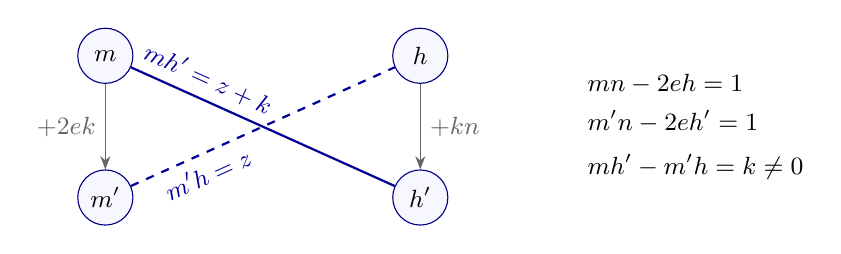
\begin{tikzpicture}[>=Stealth,every node/.style={font=\small},
  factor/.style={circle,draw=blue!50!black,fill=blue!3,
                 minimum size=7mm,inner sep=2pt}]
 \node[factor] (m) at (0,.9) {$m$};
 \node[factor] (h) at (4,.9) {$h$};
 \node[factor] (mp) at (0,-.9) {$m'$};
 \node[factor] (hp) at (4,-.9) {$h'$};
 \draw[->,gray!80!black] (m)--node[left]{$+2ek$}(mp);
 \draw[->,gray!80!black] (h)--node[right]{$+kn$}(hp);
 \draw[thick,blue!60!black] (m)--
   node[pos=.26,above,sloped]{$mh'=z+k$}(hp);
 \draw[thick,dashed,blue!60!black] (mp)--
   node[pos=.26,below,sloped]{$m'h=z$}(h);
 \node[align=left,anchor=west] at (6,0)
   {$mn-2eh=1$\\[3pt]
    $m'n-2eh'=1$\\[5pt]
    $mh'-m'h=k\ne0$};
\end{tikzpicture}
\caption{Forward determinant identities for factorizations with common
$e,n$. Cross-paired factors give $z=m'h$ and $z+k=mh'$; the vertical
arrows record signed increments, so either sign of $k$ is allowed.
The converse reconstruction, including its congruence, positivity,
and coprimality conditions, is proved in the text.}
\label{fig:determinant}
\end{figure}

Both $m$ and $m'$ are units modulo $q_k=2|k|$, so the congruence is
imposed exactly by
\begin{equation}\label{eq:typeii-character-congruence}
 \ind_{m'\equiv m\ (q_k)}
       =\frac1{\varphi(q_k)}\sum_{\chi\bmod q_k}
                                  \chi(m)\overline{\chi(m')}.
\end{equation}
Thus $\mathcal N_{\rm off}$ is a sum over $k,z$ and these characters
of terms having coefficient
\[
 \alpha_m\overline{\alpha_{m'}}\chi(m)\overline{\chi(m')}
                    a_h(h)\overline{a_h(h')},
 \qquad m'h=z,\quad mh'=z+k,
\]
with the enlarged smooth $(e,n)$ cutoffs. Their arguments are now the
exact functions
\begin{equation}\label{eq:typeii-pulled-back}
       e=\frac{m'-m}{2k},\qquad
       n=\frac{(m'-m)z}{kmm'}+\frac1m.
\end{equation}
The cutoffs are extended smoothly by zero to nonpositive arguments,
so they impose the positivity and size conditions as well.

\subsection{Smooth separation and the shifted endpoints}

On the support just obtained, $m,m'\asymp U$, $n\asymp V$, and
$h\asymp x/e$. Hence $z=m'h$ lies in
$[xL^{-C_6},xL^{C_6}]$ for a fixed $C_6$ now allowed to depend on
$K_0$. Insert a smooth dyadic partition in $z$ with $O(T)$ terms,
and denote one scale by $Z=xL^{O(1)}$. Keep its smooth cutoff
$\psi_Z(z/Z)$ outside the ensuing Fourier expansion.

For completeness, the pulled-back cutoffs have the following uniform
regularity. Put
$t_1=\log(m/U)$, $t_2=\log(m'/U)$, $t_3=\log(z/Z)$.
Multiply by fixed smooth localizations in these three variables equal
to one on the ranges in use. From \Cref{eq:typeii-pulled-back},
every derivative of $e/E$ in the $t_i$ is
$O_j(U/(|k|E))$, and every derivative of $n/V$ is
\[
                 O_j\bigl(Z/(|k|UV)+(UV)^{-1}\bigr).
\]
Both are bounded by fixed powers of $L$; moreover, the normalized
derivatives of $\eta_e,\eta_n$ have the bounds already given.
Repeated use of the chain rule therefore bounds derivatives of the
localized product cutoff by $O_j(L^{C_7(j+1)})$. Its support in
$(t_1,t_2,t_3)$ is a fixed compact box. Fourier inversion, as in
\Cref{lem:fourier-separation}, consequently represents this cutoff
with total variation $L^{O(1)}$ as a superposition of
\begin{equation}\label{eq:typeii-three-powers}
                        m^{i\xi_1}(m')^{i\xi_2}z^{i\xi_3}.
\end{equation}
Here is an explicit tail estimate. Enlarge a fixed exponent $C_8$ so
that, with $P=L^{C_8}$, the localized cutoff $F$ satisfies
$\|\partial^\alpha F\|_\infty\ll_\alpha P^{|\alpha|}$; its
zeroth derivative is bounded independently of $L$. Integration by parts
then gives
\[
 |\widehat F(\xi)|\ll_j(1+|\xi|/P)^{-j},\qquad
 \int_{\R^3}|\widehat F(\xi)|\,d\xi\ll P^3,\qquad
 \int_{|\xi|>PL}|\widehat F(\xi)|\,d\xi\ll_j P^3L^{3-j}.
\]
Thus truncation at $PL$ has uniform error $O(L^{-A})$ for every fixed
$A$, by choosing $j>A+3C_8+3$. These later exponents may depend on
$K_0$.

There is sufficient absolute control to sum these errors. If the
coefficients in \Cref{eq:typeii-separated-coefficients} and the two
$m$ sequences are replaced by their absolute values, each resulting
endpoint convolution is at most $L^{O(1)}\tau(z_*)^2$. Its product
with $W_\ell(z)$ has squared sum $O(ZL^{O(1)})$ on $z\asymp Z$.
Cauchy's inequality, also at $z+k$, therefore bounds the absolute
correlation by $ZL^{O(1)}$. This uses only
\Cref{lem:divisor-moments}. It remains true after dropping the
congruence; hence it controls the errors just described, after summing
the polynomial number of $k$ values, dyads, and character terms.

We spell out the endpoint identification to track exactly which
sequence satisfies discrepancy. Use the notation of
\Cref{eq:typeii-separated-coefficients} and fix a character $\chi$
and frequencies in \Cref{eq:typeii-three-powers}. Since $m,m'$ are
free of group primes,
\[
       z_*=m'h_*,\qquad (z+k)_*=mh'_*,\qquad
       W_\ell(z)=W_\ell(h),\quad W_\ell(z+k)=W_\ell(h').
\]
Define the invariant endpoint functions
\begin{align}
 F_0(v)&=\sum_{mpr=v_*}
   \alpha_m\chi(m)m^{i(\varrho-\xi_2)}
   \ind_{p\in I_{**},\,\Pminus(p)>W}p^{-i\sigma}\overline{c_r},
          \label{eq:typeii-first-endpoint}\\
 G_0(v)&=\sum_{mpr=v_*}
   \alpha_m\chi(m)m^{i(\xi_1+\varrho)}
   \ind_{p\in I_{**},\,\Pminus(p)>W}p^{-i\sigma}\overline{c_r}.
          \label{eq:typeii-second-endpoint}
\end{align}
Direct substitution shows that the separated summand is
\[
 \psi_Z(z/Z)z^{i(\varrho+\xi_3)}(z+k)^{-i\varrho}
       \overline{F_0(z)}G_0(z+k)W_\ell(z)W_\ell(z+k),
\]
up to scalar phases of modulus one and the Fourier coefficient.
For example, at $z=m'h$ the factor $h^{i\varrho}$ becomes
$z^{i\varrho}(m')^{-i\varrho}$, which explains the first endpoint's
power and the conjugation of $c_r$. In particular, the sequence inside
$F_0$ is the original $\alpha$, with its actual interval restriction.

Both \Cref{eq:typeii-first-endpoint,eq:typeii-second-endpoint} have
exactly the form in \Cref{eq:endpoint-form}. The character modulus
$2|k|$, all power frequencies, and the coefficient bounds are fixed
powers of $L$. The interval $I_{**}$ lies in
$[x^\tau,x^\eta]$ for fixed $0<\tau<\eta<1/4$, by
\Cref{eq:typeii-rough-slot} and the hypothesis $\eta_*<b_*/4$.
The residual $c_r$ has a fixed power bound, and no roughness condition
on $r$ is needed. The original $\alpha$ is supported on $W$-rough
integers and satisfies \Cref{eq:discrepancy}; the explicit character
and power factors are precisely the factors permitted in
\Cref{eq:endpoint-form}. Thus the discrepancy assumption has not been
silently transferred to a new coefficient sequence.

Finally set $\widetilde\psi_Z(t)=t\psi_Z(t)$. The last unweighted
correlation equals $Z$ times
\[
 \sum_{z>0,\ z+k>0}\frac{\widetilde\psi_Z(z/Z)}z
 z^{i(\varrho+\xi_3)}(z+k)^{-i\varrho}
       \overline{F_0(z)}G_0(z+k)W_\ell(z)W_\ell(z+k).
\]
This is \Cref{eq:shift-bound}, including its harmonic normalization.
Given any fixed $D_0$, \Cref{thm:shift} bounds it by $L^{-D_0}$
once the discrepancy exponent $B$ is sufficiently large. Consequently
each separated unweighted correlation is $O(ZL^{-D_0})$.
Choose $D_0$ after $K_0$, the $k$ range, all separation costs, and the
desired saving in \Cref{eq:typeii-cauchy}. The total off-diagonal
contribution is then $O(xL^{-A})$ for any prescribed fixed $A$.
Choose $B$ after this application of \Cref{thm:shift}. Together with
\Cref{eq:typeii-diagonal}, this gives
$|B_0|\ll xL^{-D_*-C_{f}-1}$. Summing its pre-Cauchy expansion
and the previously estimated tails proves \Cref{eq:typeii-bound}.
\end{proof}

\begin{remark}[Order of the precisions]\label{rem:typeii-order}
The band constants, $j_{**}$, $b_*$, coefficient bound $C$, and target
$D_*$ are fixed first. The transition functions, their total variation,
and the coefficient and diagonal exponents are independent of $K_0$;
only then is $K_0$ chosen. The smooth separation after Cauchy's
inequality and the accuracy required from \Cref{thm:shift} are fixed
next, and the required discrepancy exponent $B$ is fixed last.
Accordingly, when $\alpha$ is the difference between a test and its
rough-integer proxy, the precision of the cells defining that proxy may
be chosen after $B$, provided the proxy's coefficient bound is already
uniform in that cell precision. This is the order used in
\Cref{sec:primes}.
\end{remark}

\section{Extracting primes with smooth predecessors}\label{sec:primes}

We prove \Cref{thm:smooth}. Throughout this section $0<\delta<1/4$
is fixed. The task is to detect primes among $N_u:=2u+1$ for a positive
weight on integers $u$ all of whose prime factors are small. The
distribution estimate of \Cref{thm:typeii} will replace tests on a factor
of $N_u$ by simpler tests on rough integers. We specify the order of all
remaining parameter choices at the end of the section.

The extraction separates the composites according to their least prime
factor. A preliminary sieve retains those $N_u$ with no prime factor
below $x^{b_1}$, where $b_1>0$ is fixed and small. For a fixed small
$\kappa>0$ and least prime factors up to $x^{1/2-\kappa}$, Type II
replaces the roughness condition on the complementary factor by a
local density on ordinary integers.
Integrating these densities accounts for the composite part of the
sieve mass. The remaining composites have two prime factors close to
$x^{1/2}$; a separate upper-bound sieve makes their contribution small
with $\kappa$. Its constant must be independent of $\kappa$, so we
will establish that uniformity before making the final choices.

\subsection{The candidate and its mass}

Fix a nonnegative smooth function $\Psi$ supported in $[1,2]$ that is
bounded below by a positive constant on a closed interval of positive
length contained in $(1,2)$. In the marked weight of \Cref{sec:shifts}
take $q=1/2$ and $\ell=1$. Set
\[
 c_1=1,\quad c_2=\frac65,\quad c_3=\frac32,\quad c_4=\frac95,
 \qquad s'=\frac1{r_0(c_1+c_2)},\qquad s_j=s'2^{-j}L,
\]
where the fixed integer $r_0$ is sufficiently large that
\begin{equation}\label{eq:candidate-geometry}
 c_2s'<\delta,\qquad \frac{(r_0-1)c_1}{2}\ge c_2+1.
\end{equation}
Let $j_x$ be the largest integer with $c_1s_{j_x}\ge20T$, and let
\[
 Q_j=\{p\text{ prime}:c_1s_j\le\log p\le c_2s_j\}
 \qquad(0\le j\le j_x).
\]
At each scale for which $[c_3s_j,c_4s_j]$ lies wholly in
$[L^{1/10},L^{1/5}]$ or $[L^{3/10},L^{2/5}]$, take the primes in that
interval of logarithms as a small or big P-group, respectively.
The P-groups and the Q-bands are pairwise disjoint: the four constants
lie in the displayed order, and $c_4<2c_1$. The prime number theorem
and partial summation give fixed upper and positive lower bounds for
each of their reciprocal prime masses. Both numbers of P-groups are
comparable to $T$, and their exponent ranges and endpoint ratios meet
the hypotheses of the preceding sections.

There are $r_0$ ordered slots in each Q-band. Except for one designated
slot in a fixed band $j_{**}$, a slot contains a prime of its band. The
designated slot instead contains any integer $v$ satisfying
\[
 e^{c_1s_{j_{**}}}\le v\le e^{c_2s_{j_{**}}},\qquad \Pminus(v)>W.
\]
We always require $j_{**}\ge j_0$, where $j_0$ is a sufficiently large
fixed lower bound chosen below using only the candidate geometry.
In particular $j_{**}\ge1$. Define
\[
 a_Q(v)=\prod_{j=0}^{j_x}\frac1{r_0!}
       \#\{\text{admissible ordered Q-lists with product }v\},
 \qquad A(u)=a_Q(u_*)W_1(u).
\]
The P-free part $u_*$ and the marked weight $W_1$ are those of
\Cref{sec:shifts}. The rough slot has no P-prime divisor for large $x$,
since all P primes are less than $W$.

The candidate must have substantial ordinary mass near $x$, despite
the restrictions on all its factors. Reciprocal weights make the slot
choices independent. The band geometry leaves room for one prime in
the largest band to adjust their product to size $x$; under this
harmonic sampling, that prime supplies a local probability of order
$1/L$. The next proposition records the resulting mass and the
pointwise bound needed to convert that mass into a count of distinct
primes.

\begin{proposition}[Candidate mass]\label{prop:candidate-mass}
Put
\[
 X_A=\sum_u A(u)\Psi(u/x),\quad
 H_Q=\sum_v\frac{a_Q(v)}v,\quad
 H_P=\sum_{r:r_*=1}\frac{W_1(r)}r.
\]
There are constants $C,C_A$ depending only on the early candidate
choices such that, for sufficiently large $x$ after fixing $j_{**}$,
\begin{align}
 0\le A(u)&\le L^C\tau(u_*),
 & A(u)&\le\exp(C\sqrt L)\quad(u\asymp x),\label{eq:candidate-pointwise}\\
 H_P&\sim\exp\left(q\sum_g V_g\right),
 & X_A&\asymp\frac{x}{L}H_QH_P\gg xL^{-C_A}.
 \label{eq:candidate-mass}
\end{align}
The comparison constants in \eqref{eq:candidate-mass} can be chosen
independently of $j_{**}\ge j_0$. On the support of
$A(u)\Psi(u/x)$ every prime divisor of $u$ lies in $[L^{20},x^\delta]$.
\end{proposition}

\begin{proof}
After fixing the value of the rough slot as a divisor of $v$, the
remaining prime multiplicities determine their band assignments.
The normalized number of ordered lists in each band is at most one.
This gives $a_Q(v)\le\tau(v)$. For $v\ll x$, any possible rough-slot
divisor divides the part of $v$ supported on primes exceeding $W$.
That part has at most $O(L/\log W)=O(\sqrt L)$ prime factors counted
with multiplicity, and hence at most $\exp(O(\sqrt L))$ divisors.
Together with the pointwise bound $W_1(u)\le L^{O(1)}$ this proves
\eqref{eq:candidate-pointwise}. The claimed lower and upper bounds on
prime factors follow from the definitions, \eqref{eq:candidate-geometry},
and $\exp(L^{2/5})<x^{c_2s'}$ for large $x$.

\paragraph{Harmonic masses and the P-part.}
The Q harmonic sum factorizes into the reciprocal masses of all its
slots, divided by $r_0!$ in each band. Each pure-prime slot has mass
between two fixed positive constants. The rough-slot mass is at most
$O(L)$ and is bounded below by a fixed positive constant for
sufficiently large $x$ after fixing $j_{**}$; for the latter assertion
one may restrict that slot to primes of $Q_{j_{**}}$, which then all
exceed $W$. Since there are $O(T)$ slots,
\begin{equation}\label{eq:candidate-harmonic-size}
 L^{-C}\le H_Q\le L^C.
\end{equation}
This exponent and these eventual bounds do not depend on $j_{**}$.

For one P-group write
$F_g(q)=\prod_{p\in\mathcal P_g}(1+q/(p-1))$.
Summing over all powers of its prime divisors shows that its factor
in $H_P$ is
\begin{equation}\label{eq:marked-euler-factor}
 \frac{F_g'(q)}{V_g}
  =F_g(q)\frac1{V_g}\sum_{p\in\mathcal P_g}\frac1{p-1+q}.
\end{equation}
As $\sum_{g,p\in\mathcal P_g}p^{-2}=o(1)$ and $V_g$ is bounded
above and below, multiplying \eqref{eq:marked-euler-factor} proves
the asymptotic for $H_P$. It also proves the useful exact inequality
\begin{equation}\label{eq:mask-euler-comparison}
 H_P\ge\prod_{p\text{ a P prime}}\left(1+\frac q{p-1}\right),
\end{equation}
since $p-1+q\le p$.

The harmonic P-measure assigns negligible mass to $r>x^\sigma$ for
any fixed $\sigma>0$. Indeed set $\xi=L^{-2/5}$ and replace $p^{-1}$
by $p^{-1+\xi}$ in the preceding Euler calculation. Since
$p^\xi\le e$ for every P prime, the tilted factor of each group is
bounded by a fixed constant. Consequently
\begin{equation}\label{eq:candidate-P-tail}
 \sum_{r>x^\sigma,\ r_*=1}\frac{W_1(r)}r
 \le \exp(-\sigma L^{3/5})L^{O(1)}.
\end{equation}

\paragraph{Localizing the product near $x$.}
Normalize the independent P choice and all the Q-slot harmonic
choices by $H_PH_Q$, and denote their product by $U$. Then
\[
 X_A=H_PH_Q\,\E\{U\Psi(U/x)\}.
\]
For the upper comparison we need probability $O(1/L)$ throughout
$x\le U\le2x$; for the lower comparison we need probability
$\gg1/L$ where $U/x$ lies in the positivity interval of $\Psi$.
Both are intervals of bounded length for $\log U$. The P-tail
estimate ensures that the P-part does not move the product out of
reach of the largest Q-band.
Condition on everything except one pure-prime slot in $Q_0$.
The prime number theorem implies that its logarithm falls in any
interval of bounded length with probability $O(1/L)$, uniformly in
the location of that interval. Thus
$\Prob(x\le U\le2x)=O(1/L)$, giving the upper mass bound.

Here is a uniform lower bound. The sum of the midpoints of all the
infinite Q-bands, counting their $r_0$ slots, is exactly
\[
 \sum_{j\ge0}r_0\frac{c_1+c_2}{2}s'2^{-j}L=L.
\]
Let $\Delta=(c_2-c_1)s'L$, the logarithmic width of the free slot.
Choose a fixed prefix of bands so long that the sum of all later
band widths and midpoints is less than $\Delta/24$. Within that
prefix, restrict all slots except the free slot to fixed small
relative neighborhoods of their midpoints, so that their total
deviation is at most $\Delta/24$. This event has probability bounded
below by a positive constant: it involves only a fixed number of
pure-prime slots. Choose $j_0$ larger than the prefix length so that
the exceptional slot is always in the unrestricted tail. Its full
range obeys the same deterministic tail bound. Missing bands after
$j_x$ also obey that bound. Finally restrict the P choice to
$\log r\le\Delta/12$, at negligible loss by
\eqref{eq:candidate-P-tail}.
On this event, a target interval for $\log U$ coming from the
positivity interval of $\Psi$ gives an interval of fixed positive
length for the free slot, lying a distance at least $\Delta/4$
from its range endpoints for large $x$. The prime number theorem
gives conditional probability $\gg1/L$. Multiplying by $U\asymp x$
proves the lower comparison in \eqref{eq:candidate-mass}. This
argument uses no property of the tail distribution beyond its
range, so its constants are uniform in the later choice of
$j_{**}$. The final lower bound follows from
\eqref{eq:candidate-harmonic-size} and the Euler calculation.
\end{proof}

\subsection{Congruence distribution and the preliminary sieve}

For odd squarefree $d$ define
\[
 r(d)=\sum_{d\mid N_u}A(u)\Psi(u/x)-\frac{X_A}{\varphi(d)}.
\]
\begin{proposition}[Type I distribution]\label{prop:typeI}
For every fixed $\vartheta<1/2$ and $D>0$,
\begin{equation}\label{eq:typeI-bound}
 \sum_{\substack{d\le x^\vartheta\\d\text{ odd and squarefree}}}
 |r(d)|\ll xL^{-D}+X_AL^{-18}.
\end{equation}
\end{proposition}

\begin{proof}
The congruence $2u+1\equiv0\pmod d$ specifies a unit class for $u$.
Use character orthogonality on that class. Replacing the principal
coprime mass by $X_A$ has total cost at most $X_AL^{-18}$, because
for each supported $u$,
\[
 \sum_{\substack{d\le x^\vartheta\\(d,u)>1}}
       \frac{\mu^2(d)}{\varphi(d)}
 \le \sum_{p\mid u}\frac1{p-1}
             \sum_{d'\le x}\frac{\mu^2(d')}{\varphi(d')}
 \ll L^{-18}.
\]
Here every $p\mid u$ is at least $L^{20}$, there are at most
$O(L/\log L)$ such primes, and the last sum is $O(L)$ by its Euler
product and Mertens' theorem.

Extract one fixed $Q_0$ slot, as in the proof of
\Cref{prop:candidate-mass}, to write
\[
 A(u)=\sum_{\substack{pr=u\\p\in Q_0}}b(r),
 \qquad 0\le b(r)\le L^{O(1)}\tau(r).
\]
Split $p,r$ into dyads of sizes $P,U$ with $PU\asymp x$.
There is a fixed $a>0$ such that $x^a\ll P,U\ll x^{1-a}$ in
every contributing dyad. A nonprincipal character modulo squarefree
$d$ is induced by a primitive nonprincipal character modulo $f>1$,
where $d=hf$ and $(h,f)=1$. It acts as that primitive character
together with the restrictions $(p,h)=(r,h)=1$, and
$\varphi(d)=\varphi(h)\varphi(f)$.

Fix $h$. On conductors $f\asymp R>L^{C'}$, separate
$\Psi(pr/x)$ by Mellin inversion, which has bounded integrated
absolute cost. For each resulting twist, \Cref{thm:large-sieve},
Cauchy--Schwarz, and \Cref{lem:divisor-moments} give
\begin{align*}
 &\sum_{f\asymp R}\frac1{\varphi(f)}
     \sum_{\chi\bmod f}^{*}
     \left|\sum_{p\asymp P}a_p\chi(p)\right|
     \left|\sum_{r\asymp U}b_r\chi(r)\right|\\
 &\hspace{12mm}\ll
  \frac{L^{O(1)}}R\sqrt{(P+R^2)(U+R^2)PU}\\
 &\hspace{12mm}\ll xL^{O(1)}
       \left(R^{-1}+P^{-1/2}+U^{-1/2}+R/\sqrt x\right).
\end{align*}
The coefficients include coprimality to $h$ and unit-modulus
Mellin twists, so their squared sums are $O(P)$ and
$UL^{O(1)}$. Discarding $(h,f)=1$ and squarefreeness only enlarges
this positive bound. Summing dyads and $1/\varphi(h)$ costs a fixed
power of $L$. Since $R\le x^\vartheta$, a sufficiently large $C'$
gives any prescribed logarithmic saving.

For $1<f\le2L^{C'}$, fix $r$ and apply \Cref{thm:sw} to the
$p$-sum with the original smooth cutoff $\Psi(pr/x)$, using partial
summation. The nonprincipal character sum is $O_A(PL^{-A})$ for
arbitrary fixed $A$. Omitting primes dividing $h$ costs only $O(1)$
terms, since such primes in this range are at least $x^a$ and
$h\le x^\vartheta$. Their total cost after summing $r$, moduli and
dyads is $x^{1-a}L^{O(1)}$. The remaining costs are fixed powers of
$L$, absorbed by choosing $A$ large. This proves
\eqref{eq:typeI-bound}.
\end{proof}

Define
\[
 V(y)=\prod_{p\le y}(1-1/p),\qquad
 V_1(y)=\prod_{3\le p\le y}(1-1/(p-1)),\qquad
 \mathfrak S=2\prod_{p\ge3}\left(1-\frac1{(p-1)^2}\right)>0.
\]
Writing $\gamma_E$ for Euler's constant, Mertens' theorem gives
\begin{equation}\label{eq:sieve-products}
 V(y)\sim\frac{e^{-\gamma_E}}{\log y},\qquad
 V_1(y)\sim\mathfrak S V(y).
\end{equation}
We will choose a small fixed $0<\kappa<1/50$ and then a sufficiently
small fixed $b_1>0$. Set $b_*=b_1/3$ for \Cref{thm:typeii}, and
eventually require
\begin{equation}\label{eq:rough-slot-placement}
 j_{**}\ge j_0,\qquad c_2s'2^{-j_{**}}<b_*/4.
\end{equation}
Apply \Cref{lem:sieve} to odd prime divisors of $N_u$ up to $x^{b_1}$,
with density $g(p)=1/(p-1)$ and the remainders from
\Cref{prop:typeI}. Take
\[
 h=2\left\lfloor\frac1{40b_1}\right\rfloor,
 \qquad \vartheta=\frac12-\frac\kappa2.
\]
For sufficiently small $b_1$, $h$ is large enough for that lemma and
$b_1(4h+2)<\vartheta$. Choose $D>C_A+10$ in
\eqref{eq:typeI-bound}. It follows that
\begin{equation}\label{eq:presieve-mass}
 \sum_{\Pminus(N_u)>x^{b_1}}A(u)\Psi(u/x)
 \ge \frac{\mathfrak S X_A}{L}
   \left\{\frac{e^{-\gamma_E}}{b_1}
                 (1-O(e^{-c/b_1}))+o(1)\right\}.
\end{equation}
The constants in the exponential error are uniform for small
$b_1$ and $0<\kappa<1/50$.

\subsection{Proxies with character and Mellin discrepancy}

We now construct the coefficients that Type II will compare with the
factor tests. The proxy has exactly the same sum as the test on each
short logarithmic cell, but is constant among the $W$-rough integers
in that cell. This count matching handles the principal
characters; prime estimates and the elementary sieve will give the
nonprincipal cancellation independently of Type II. The cell width may
therefore be chosen after Type II specifies its required discrepancy.

At fixed $b_1,\kappa$, partition $(b_1,1/2-\kappa]$ into finitely
many exponent bins $(\gamma,\gamma']$. Their mesh will be chosen
later. On the factor ranges used below consider the tests
\[
 I_\gamma(m)=\ind_{\Pminus(m)>x^\gamma},\qquad
 I_{\mathrm{pr}}(m)=\ind_{m\text{ prime}}.
\]
Every such range lies between two fixed positive powers of $x$;
in particular we can work throughout the ambient interval
$[x^{b_1/4},x^{1-b_1/4}]$. Put $\Delta_L=L^{-S}$, with $S$ a
fixed precision to be chosen last. Partition the logarithmic axis
into intervals of width $\Delta_L$. For a full cell
$C_Y=(Y,e^{\Delta_L}Y]$ meeting this ambient interval, set
\begin{equation}\label{eq:proxy-definition}
 c_I(C_Y)=\frac{\sum_{m\in C_Y}I(m)}
                   {\#\{m\in C_Y:\Pminus(m)>W\}},\qquad
 B_I(m)=c_I(C_Y)\ind_{\Pminus(m)>W}\quad(m\in C_Y).
\end{equation}
The counts defining $c_I$ are full-cell counts even when the factor
range cuts a cell. Range restrictions are imposed afterwards.

\begin{lemma}[Proxy discrepancy]\label{lem:proxy-discrepancy}
The denominators in \eqref{eq:proxy-definition} are positive for
large $x$. Moreover $0\le B_I\le1$. Given any fixed discrepancy
exponent $B$, taking $S>2B+3$ makes
\[
 \alpha_m=(I(m)-B_I(m))\ind_{m\in K}
\]
satisfy \eqref{eq:discrepancy}, uniformly for every interval $K$
inside a dyad in the stated factor ranges, for each of the finitely
many tests above. Thus the coefficient bound required by
\Cref{thm:typeii} is independent of $S$.
\end{lemma}

\begin{proof}
Use \Cref{lem:sieve} on ordinary integers in a cell with $z=W$,
$g(p)=1/p$, and $h=2\lceil T^2\rceil$. Each divisibility remainder
is $O(1)$, and the sieve level is
\[
 D_W=W^{4h+2}=\exp(O(\sqrt L\,T^2))=x^{o(1)}.
\]
Since $Y\gg x^{b_1/4}$, uniformly for these cells,
\begin{equation}\label{eq:proxy-denominator}
 \#\{m\in C_Y:\Pminus(m)>W\}
  =(e^{\Delta_L}-1)YV(W)(1+O(e^{-T^2}))+O(D_W)
  \sim\Delta_L YV(W).
\end{equation}
Both actual tests select subsets of these rough integers for large
$x$: for the prime test all integers in the cell exceed $W$, and
for the other tests $x^\gamma>W$. Hence $0\le c_I\le1$ exactly.

Every prime divisor of a modulus $r\le L^B$ is below $W$, so a
principal character is one throughout the support of $\alpha$.
On a full cell the unweighted sum of $I-B_I$ is zero. For
$f(t)=t^{iv-1}$, $|v|\le L^B$, its variation on that cell is at most
$O((1+|v|)\Delta_L/Y)$. The absolute harmonic mass on a dyad is
$O(1)$ (even the weaker $O(L^{1/2})$ would suffice). Consequently
the full cells contribute $O(L^{B-S})$. Intersecting the test
interval in \eqref{eq:discrepancy} with $K$ leaves at most two
partial cells; their combined harmonic mass is
$O(L^{-S}+x^{-b_1/4})$. These bounds imply the principal-character
case with room to spare when $S>2B+3$.

For a nonprincipal character, first treat the actual roughness
test. Each admitted integer has a unique nondecreasing list of
at most $O(1/b_1)$ prime factors. Fix the first $l-1$ factors and
sum over the last prime. Its order restriction, its lower bound
$x^\gamma$, and the interval restriction on the full product
intersect in one prime interval. Its endpoints lie between
$x^\gamma$ and $x^2$. By \Cref{thm:sw} and partial summation, the
harmonic sum of this prime against a nonprincipal character and
the twist $p^{iv}$ has arbitrarily strong logarithmic saving,
uniformly for a prescribed logarithmic bound on the modulus and
$v$. The reciprocal masses of the remaining factors are bounded
in terms of $b_1$, because
$\sum_{x^\gamma<p\le x^2}p^{-1}=O_{b_1}(1)$.
Summing the bounded number of list lengths preserves the saving.
Repeated primes are included by the nondecreasing enumeration.
Imprimitive nonprincipal characters give the same estimate via
their nonprincipal primitive characters; primes dividing the
modulus are too small to occur. For $I_{\mathrm{pr}}$ this is the
same argument with one prime.

It remains to treat the proxy. For every subinterval $J'$ of a
cell and every unit class $a\pmod r$, apply \Cref{lem:sieve} to
that class, omitting primes dividing $r$ from the sieve. The CRT
gives an $O(1)$ remainder at each squarefree sieve product. Since
all prime divisors of $r$ are below $W$, the main term is
\[
 \frac{|J'|}{r}\prod_{\substack{p\le W\\p\nmid r}}(1-1/p)
 =\frac{|J'|V(W)}{\varphi(r)}.
\]
Thus, also for very short $J'$ as an absolute-error assertion,
\begin{equation}\label{eq:rough-class-count}
 \#\{m\in J':m\equiv a\pmod r,\ \Pminus(m)>W\}
 =\frac{|J'|V(W)}{\varphi(r)}(1+O(e^{-T^2}))+O(D_W).
\end{equation}
Summing against a nonprincipal character cancels the common main
term, and bounds the remaining sum by
$O(|J'|V(W)e^{-T^2}+\varphi(r)D_W)$. Multiply by the cell constant
$c_I\le1$ and use partial summation against $m^{iv-1}$.
The number of cells is at most $O(L^{S+1})$; the moduli and twists
cost fixed powers of $L$. The first error therefore remains
smaller than every fixed negative power of $L$, and the second
is $x^{-b_1/4+o(1)}$ times a fixed power of $L$. This proves the
nonprincipal assertion, including all interval truncations.
\end{proof}

For all later applications, prescribe the saving in
\Cref{thm:typeii} large enough that its errors, after the required
dyadic decompositions, are $o(X_A/L)$. Its coefficient exponent
is fixed before $S$, by \Cref{lem:proxy-discrepancy}; obtain its
required discrepancy exponent and then choose $S$. There are
only finitely many test types, so the same $S$ works for all.

\subsection{The local densities and their integral identity}

The proxy discrepancy allows replacement of a factor test, while its
local density controls the size of the replacement. We need ordinary
rough-integer counts for the cofactor left after a least prime factor
has been selected. For a product of $l$ primes, their logarithms,
divided by $L$, sum to the logarithmic size of that cofactor. This
leads to the following finite sum of integrals over those logarithms.

For $w>\gamma>0$ define
\begin{equation}\label{eq:rough-density-definition}
 D_\gamma(w)=\frac1w+
 \sum_{l\ge2}\frac1{l!}
  \int_{\substack{t_i\ge\gamma\ (1\le i<l)\\
                    \sum_{i<l}t_i\le w-\gamma}}
  \frac1{w-\sum_{i<l}t_i}\prod_{i<l}\frac{dt_i}{t_i}.
\end{equation}
Only finitely many terms are nonzero. On compact subsets of
$w>\gamma>0$ the functions are jointly continuous, including at
thresholds $w=l\gamma$: the integrands have bounded denominators
and the moving boundaries have measure zero.

These are Buchstab's rough-number densities in logarithmic
coordinates, and the minimum-coordinate decomposition below is the
corresponding Buchstab identity \cite{Buchstab1937}.
We derive the short-cell bounds and integral identity needed here directly.

\begin{lemma}[Proxy density bounds]\label{lem:proxy-densities}
For the prime proxy in the interval
$x^{1/2-2\kappa}\le m\le x^{1/2+2\kappa}$,
\begin{equation}\label{eq:prime-proxy-size}
 c_{\mathrm{pr}}(m)\le\frac{C}{LV(W)},
\end{equation}
where $C$ is absolute for $0<\kappa<1/50$. If $mn=N_u$ on the
support of $\Psi(u/x)$ and $\log n/L\in(\gamma,\gamma']$, then
\begin{equation}\label{eq:rough-proxy-size}
 c_\gamma(m)\le
 \frac{\sup_{\gamma\le a\le\gamma'}D_\gamma(1-a)+o(1)}{LV(W)}.
\end{equation}
At fixed $b_1$ one also has
\begin{align}
 \int_{b_1}^{1/2}D_\alpha(1-\alpha)\frac{d\alpha}{\alpha}
       &=D_{b_1}(1)-1,\label{eq:density-integral}\\
 D_{b_1}(1)&\le\frac{e^{-\gamma_E}}{b_1}
                 (1+O(e^{-c/b_1})).\label{eq:density-sieve-upper}
\end{align}
The integrand at the endpoint $\alpha=1/2$ is understood by
its left limit; changing that endpoint value has no effect.
\end{lemma}

\begin{proof}
The prime number theorem with an arbitrarily large logarithmic
error, applied at both endpoints of a cell, gives
\[
 \#\{p\in(Y,e^{\Delta_L}Y]\}
   =(1+o(1))\frac{\Delta_LY}{\log Y}.
\]
For $w=\log Y/L\in[0.46+o(1),0.54+o(1)]$, divide by
\eqref{eq:proxy-denominator} to obtain
\eqref{eq:prime-proxy-size} with an absolute eventual constant.
Increasing fixed $S$ changes the threshold for $x$, not that
constant.

More generally, uniformly on compact sets with $\gamma\ge b_1$,
$w-\gamma$ bounded below positively, and $w$ bounded above, the
number of integers rough above $x^\gamma$ in the cell is at most
\begin{equation}\label{eq:rough-cell-density}
 (D_\gamma(w)+o(1))\frac{\Delta_LY}{L}.
\end{equation}
To see this, repeated prime factors contribute at most
\[
 \sum_{p>x^\gamma}\left\lfloor\frac{2Y}{p^2}\right\rfloor
 \ll Yx^{-b_1}=o(\Delta_LY/L).
\]
Count the squarefree remaining integers by ordered lists of $l$
primes with weight $1/l!$, where $l$ is bounded in terms of
$b_1$. Fix the first $l-1$ primes, write $Q=\prod_{i<l}p_i$ and
$t_i=\log p_i/L$. A last prime can occur only when
$\sum_{i<l}t_i\le w-\gamma+O(\Delta_L/L)$. Dropping its lower
cutoff, its count is at most
\[
 (1+o(1))\frac{\Delta_LY}{LQ(w-\sum_{i<l}t_i)}.
\]
The prime number theorem is uniform here because
$Y/Q\ge x^\gamma/2$, and its logarithmic accuracy is chosen
larger than $S+3$. The reciprocal-prime measures for the remaining
slots converge to $dt_i/t_i$. A finite grid approximation proves
uniform convergence of the resulting integrals: denominators
stay bounded away from zero, while strips around the moving
hyperplane boundary have uniformly vanishing volume. This is
exactly \eqref{eq:rough-density-definition}, proving
\eqref{eq:rough-cell-density}. In the application
$w=1-\log n/L+o(1)$ and $w-\gamma\ge2\kappa+o(1)$.
Continuity, followed by division by
\eqref{eq:proxy-denominator}, proves \eqref{eq:rough-proxy-size}.

For \eqref{eq:density-integral}, write the $l$th term of
$D_{b_1}(1)$, $l\ge2$, on the simplex
\[
 t_1+\cdots+t_l=1,\qquad t_i\ge b_1,
 \qquad \frac1{l!}\frac{dt_1\cdots dt_{l-1}}{t_1\cdots t_l}.
\]
This measure is invariant under every permutation of the $l$
coordinates: exchanging a dependent and an independent coordinate
has absolute Jacobian one. Except on a null set exactly one
coordinate is the minimum, say $\alpha$. Select that coordinate
in $l$ ways. Its measure is $d\alpha/\alpha$, and the remaining
coordinates, with sum $1-\alpha$ and lower bound $\alpha$, give
the $(l-1)$-factor term of $D_\alpha(1-\alpha)$. The coefficient
$l/l!$ is precisely $1/(l-1)!$. Summing proves the identity; the
one-prime term of $D_{b_1}(1)$ equals one.

For the inequality, first obtain a lower density for ordinary
rough integers in $(x,2x]$. Ordered prime lists with weight $1/l!$
assign at most unit mass to every integer, including those with
repetitions. For $l\ge2$ restrict the first $l-1$ logarithms to
$\sum t_i<1-b_1-\eta$, with $\eta>0$ fixed, and sum the last prime
over $(x/Q,2x/Q]$. It is then wholly above the threshold. The
prime number theorem and the same reciprocal-measure convergence
give the corresponding integrals times $x/L$. Include the
one-prime term and let $\eta$ decrease to zero. Null boundaries
give
\[
 \liminf_{x\to\infty}\frac Lx
        \#\{x<m\le2x:\Pminus(m)>x^{b_1}\}\ge D_{b_1}(1).
\]
On the other hand \Cref{lem:sieve}, with $g(p)=1/p$, $O(1)$
remainders and $h=2\lfloor1/(40b_1)\rfloor$, bounds this count by
\[
 xV(x^{b_1})(1+O(e^{-c/b_1}))+O(x^{b_1(4h+2)}).
\]
Its remainder is $o(x/L)$ for small $b_1$, and
\eqref{eq:sieve-products} proves \eqref{eq:density-sieve-upper}.
\end{proof}

The term $1$ in \eqref{eq:density-integral} is the one-prime
contribution to $D_{b_1}(1)$. Selecting a least prime factor accounts
for all the other terms. Thus the integral provides the composite
density to subtract from the preliminary sieve mass, with the
one-prime term left over. These are densities for ordinary rough
integers used in the proxies; their application to $N_u$ uses Type II
followed by Type I and the sieve.

\subsection{Subtracting composites away from balance}

Consider a composite $N_u$ counted in \eqref{eq:presieve-mass},
whose least prime factor is at most $x^{1/2-\kappa}$. Its least
prime factor $p$ lies in one bin $(x^\gamma,x^{\gamma'}]$, and
$m=N_u/p$ satisfies $\Pminus(m)>x^\gamma$. Its contribution is
therefore bounded by
\[
 \sum_{\substack{mp=N_u\\x^\gamma<p\le x^{\gamma'}\text{ prime}}}
       A(u)\Psi(u/x)I_\gamma(m).
\]
All contributing dyads of $m,p$ lie between $x^{b_*}$ and
$x^{1-b_*}$ for large $x$, with $b_*=b_1/3$: the factors bounded
by constants in $N_u\asymp x$ are absorbed by the strict exponent
slack. Apply \Cref{thm:typeii} with
$\alpha=I_\gamma-B_\gamma$ restricted to each actual cofactor
range, and $\beta$ the prime indicator restricted to its bin and
dyad. \Cref{lem:proxy-discrepancy} supplies precisely its
discrepancy hypothesis. Replacing $I_\gamma$ by $B_\gamma$ costs
$o(X_A/L)$ in total.

For a prime $p>W$, the condition that $m=N_u/p$ be rough above
$W$ is equivalent to $\Pminus(N_u)>W$. By
\eqref{eq:rough-proxy-size}, the resulting upper bound reduces
to a constant divided by $LV(W)$ times
\[
 \sum_{x^\gamma<p\le x^{\gamma'}}
       \sum_{\substack{p\mid N_u\\\Pminus(N_u)>W}}
                     A(u)\Psi(u/x).
\]
For each such $p$, sieve the odd primes up to $W$, using the base
mass $X_A/(p-1)$, density $1/(l-1)$, and remainders $r(pd)$.
Take $h=2\lceil T^2\rceil$ in \Cref{lem:sieve}. All products
$pd$ are at most $x^{1/2-\kappa+o(1)}$, which is below the
Type I level $x^{1/2-\kappa/2}$. Moreover different pairs $(p,d)$
give different products: $p>W$ is their unique prime factor above
$W$. Thus \eqref{eq:typeI-bound} bounds the summed remainders
without any divisor multiplicity loss. We obtain
\begin{align*}
 &\sum_{x^\gamma<p\le x^{\gamma'}}
       \sum_{\substack{p\mid N_u\\\Pminus(N_u)>W}}
                  A(u)\Psi(u/x)\\
 &\hspace{12mm}=X_AV_1(W)
          \sum_{x^\gamma<p\le x^{\gamma'}}\frac1{p-1}
                   +o(X_AV(W)).
\end{align*}
Since the reciprocal sum tends to $\log(\gamma'/\gamma)$,
the composite contribution of the bin is at most
\begin{equation}\label{eq:unbalanced-bin}
 \frac{\mathfrak S X_A}{L}
 \left\{\sup_{\gamma\le a\le\gamma'}D_\gamma(1-a)
                    \log(\gamma'/\gamma)+o(1)\right\}.
\end{equation}
At fixed $b_1,\kappa$, joint continuity in
\Cref{lem:proxy-densities} permits a sufficiently fine fixed mesh
such that the sum of these constants is at most
\[
 \int_{b_1}^{1/2-\kappa}D_\alpha(1-\alpha)
                       \frac{d\alpha}{\alpha}+\frac1{10}.
\]
Subtracting \eqref{eq:unbalanced-bin} from
\eqref{eq:presieve-mass} and using
\Cref{eq:density-integral,eq:density-sieve-upper} leaves at least
\begin{equation}\label{eq:prime-balanced-mass}
 \frac{\mathfrak S X_A}{L}
      \left\{1-\frac1{10}
               -O(b_1^{-1}e^{-c/b_1})+o(1)\right\}
 \ge \frac{\mathfrak S X_A}{2L}
\end{equation}
on primes and composites with least prime factor exceeding
$x^{1/2-\kappa}$, provided $b_1$ is sufficiently small.

\subsection{A uniform upper bound for balanced composites}

If a composite $N_u\ll x$ has least prime factor above
$x^{1/2-\kappa}$, it has exactly two prime factors counted with
multiplicity, because $3(1/2-\kappa)>1$. Both factors belong,
for large $x$, to
\[
 \mathcal B_\kappa=[x^{1/2-2\kappa},x^{1/2+2\kappa}].
\]
We may overcount them by ordered pairs $m,n$ of primes in that
range with $mn=N_u$. Replace the first prime indicator by its
proxy using \Cref{thm:typeii}, then replace the second using the
same theorem with the factor roles exchanged. The remaining
coefficient in the second application is a proxy bounded by one.
All required discrepancy and range hypotheses follow from
\Cref{lem:proxy-discrepancy}, as before. By
\eqref{eq:prime-proxy-size}, the resulting upper bound is
$o(X_A/L)$ plus
\begin{equation}\label{eq:balanced-proxy-bound}
 \frac{C}{L^2V(W)^2}
 \sum_{\substack{m,n\in\mathcal B_\kappa,\ mn=2u+1\\
                   \Pminus(m)>W,\ \Pminus(n)>W}}
                     A(u)\Psi(u/x).
\end{equation}
We now bound this positive sum with a constant independent of
$\kappa,b_1,j_{**}$ and $S$.

More precisely, we will show that each dyadic pair with $mn\asymp x$
contributes $O(X_AV(W)^2)$. There are only $O(\kappa L+1)$ such
pairs in the indicated range, so the prefactor in
\eqref{eq:balanced-proxy-bound} will give an
$O((\kappa+L^{-1})X_A/L)$ bound. To prove the dyadic estimate, we
retain a small divisor of $u$ from its Q-slots and P-marks. After
discarding the remaining large Q-prime restrictions, a two-variable
sieve enforces roughness of $m,n$ and the remaining small-prime
restrictions on $u=(mn-1)/2$.

Choose a fixed large index $j'$ and then $\theta$ in the gap
\begin{equation}\label{eq:micro-choice}
 c_2s'2^{-j'}<\theta<c_1s'2^{-j'+1},\qquad
 10\theta\le\frac1{20},\qquad
 \sum_{j\ge j'}r_0c_2s'2^{-j}\le\frac1{25}.
\end{equation}
Such a gap exists because $c_2<2c_1$. These choices depend only
on the candidate geometry. Increase the early lower bound $j_0$
to ensure $j_0\ge j'$, so the rough slot is in a band $j\ge j'$.
Call these the micro bands. Write $H_Q^{\mathrm{mic}}$ for the
Q harmonic mass using just these bands. Omitting the finitely
many fixed bands $j<j'$ gives
\begin{equation}\label{eq:micro-harmonic-comparison}
 H_Q^{\mathrm{mic}}\ll H_Q
\end{equation}
with a constant independent of $j_{**}$.

An assignment consists of the complete ordered Q-lists in the
micro bands, including the rough slot, and one marked prime
from every P-group. Give it weight
\[
 \lambda_{\mathrm{assgn}}
  =\prod_{j=j'}^{j_x}\frac1{r_0!}\prod_g\frac1{V_g},
\]
and let $D_1$ be the product of all its entries, with
multiplicity. The Q contribution has size at most $x^{1/25}$ by
\eqref{eq:micro-choice}; the P marks have product
$\exp(O(TL^{2/5}))=x^{o(1)}$. Thus
\begin{equation}\label{eq:assignment-size}
 D_1\le x^{1/20},\qquad
 \sum_{\mathrm{assgn}}\frac{\lambda_{\mathrm{assgn}}}{D_1}
            =H_Q^{\mathrm{mic}},\qquad
 \sum_{\mathrm{assgn}}\lambda_{\mathrm{assgn}}
            \le x^{1/20}H_Q^{\mathrm{mic}}.
\end{equation}
In the middle identity the harmonic sum of the normalized
P mark in each group is exactly $V_g^{-1}\sum p^{-1}=1$.

The damping in $W_1$ can also be retained in this upper bound.
Once one P-prime per group is marked in $D_1$, every additional
distinct P-prime divisor of $u$ contributes a factor $q$. We represent
these factors by independent random permissions for those primes;
averaging the permissions recovers exactly the damping.

For each assignment, ban every odd non-P prime $l\le x^\theta$
not dividing $D_1$. For each P prime not dividing $D_1$,
independently allow it with probability $q$ and otherwise ban it.
Primes dividing $D_1$ are never banned.
All P primes are below $x^\theta$ and indeed below $W$ for large
$x$. We have the pointwise majorant
\begin{equation}\label{eq:mask-majorant}
 A(u)\le
 \sum_{\mathrm{assgn}}\lambda_{\mathrm{assgn}}
     \ind_{D_1\mid u}\,
     \E_{\mathrm{mask}}\ind_{\{l\nmid u\text{ for every banned }l\}}.
\end{equation}
To verify it, expand $A(u)$ into Q-lists and one P mark per group.
For every genuine list the divisibility $D_1\mid u$ holds, and
every non-P prime divisor of $u$ below $x^\theta$ occurs in
$D_1$: omitted Q-bands contain only pure primes above $x^\theta$.
The micro Q product has no P factors, so $D_1$ contains exactly
one distinct P prime per group. For such a genuine list, the
mask expectation is $q^{\omega(u)-s}$, precisely the damping in
$W_1(u)$. Once the micro entries are fixed, the normalized
number of omitted pure-prime lists with any fixed residual
product is at most one. Explicitly, a band with prime
multiplicities $a_p$ contributes $\prod_p1/a_p!\le1$; disjointness
prevents alternative band assignments. Dropping these residual
restrictions proves \eqref{eq:mask-majorant}.

Fix now a pair of dyads $m\asymp M_1$, $n\asymp M_2$ meeting
the product support $mn\asymp x$, an assignment, and a mask.
Since $D_1$ is odd, $D_1\mid u$ and $mn=2u+1$ imply
$mn\equiv1\pmod{D_1}$. We may drop parity and use this congruence
to bound the number of pairs in the full dyadic box. For an odd
prime $l\le z':=x^\theta$ with $l\nmid D_1$, the bad events are
\[
 mn\equiv0\pmod l\quad(l\le W),\qquad
 mn\equiv1\pmod l\quad(l\text{ banned}).
\]
The two residue sets are disjoint and contain respectively
$2l-1$ and $l-1$ pairs. Put
\[
 \nu(l)=(2l-1)\ind_{l\le W}+(l-1)\ind_{l\text{ banned}},
 \qquad g(l)=\nu(l)/l^2.
\]
These densities satisfy the hypotheses of \Cref{lem:sieve}
uniformly in assignment and mask: $g(l)\le3/l$, and for $l\ge3$
they are bounded away from one. The base mass is the product
of the two real side lengths times $\varphi(D_1)/D_1^2$.

For a squarefree product $d$ of the sieve primes, the CRT gives
exactly $\varphi(D_1)\nu(d)$ residue pairs modulo $D_1d$, including
when $D_1$ has prime-power factors. Each pair of residue classes
has lattice count equal to its area term with error
\[
 O\left(1+\frac{M_1+M_2}{D_1d}\right).
\]
As $\nu(d)\le d\,3^{\omega(d)}$ and $\varphi(D_1)\le D_1$, the
sum of absolute remainders up to $D=(z')^{10}=x^{10\theta}$ is
\begin{equation}\label{eq:pair-lattice-error}
 \ll L^{O(1)}\bigl((M_1+M_2)D+D_1D^2\bigr)
 \le L^{O(1)}\bigl((M_1+M_2)x^{1/20}+D_1x^{1/10}\bigr).
\end{equation}
Here the ordinary $\omega(d)$ occurs only in this elementary
divisor bound; its sums follow, for example, from
$3^{\omega(d)}\le\tau_3(d)$, where $\tau_3(d)$ counts ordered triples
of positive integers with product $d$. Apply the upper-bound version of
\Cref{lem:sieve} with $h=2$.

We record its Euler product explicitly. A banned prime below $W$
has factor $1-3/l+2/l^2$, and a banned prime above $W$ has
factor $1-1/l+1/l^2$. Each is at most
\[
 (1-1/l)^{1+2\ind_{l\le W}}(1+O(l^{-2})).
\]
An allowed P prime has factor $(1-1/l)^2$, so it requires one
compensating factor $(1-1/l)^{-1}$. Omitting the prime 2 changes
only an absolute constant, as does the convergent product of
the $1+O(l^{-2})$ factors. Removed primes dividing $D_1$ require
at most three compensating factors. Therefore
\begin{equation}\label{eq:pair-sieve-product}
 \prod_{\substack{3\le l\le z'\\l\nmid D_1}}(1-g(l))
 \le C V(W)^2V(z')
       \prod_{l\mid D_1}(1-1/l)^{-3}
       \prod_{\substack{p\text{ allowed}\\p\nmid D_1}}(1-1/p)^{-1}.
\end{equation}
Every prime dividing $D_1$ is at least $L^{20}$, so
$D_1\le x^{1/20}$ makes its compensating product uniformly
bounded. The expectation of the last product is
\[
 \prod_{\substack{p\text{ a P prime}\\p\nmid D_1}}
       \left(1-q+\frac q{1-1/p}\right)
 =\prod_{\substack{p\text{ a P prime}\\p\nmid D_1}}
       \left(1+\frac q{p-1}\right)\le H_P
\]
by \eqref{eq:mask-euler-comparison}.

Since $\varphi(D_1)/D_1^2\le1/D_1$, sum the main sieve terms over
assignments using \eqref{eq:assignment-size}, and bound $\Psi$
by its fixed supremum. Their contribution on this dyadic pair is
\[
 \ll xV(W)^2V(x^\theta)H_Q^{\mathrm{mic}}H_P
 \ll X_AV(W)^2,
\]
by \Cref{eq:candidate-mass,eq:micro-harmonic-comparison} and
$V(x^\theta)\ll1/L$. To sum the error
\eqref{eq:pair-lattice-error}, use
$M_i\ll x^{0.54}$ and \eqref{eq:assignment-size}. The result is
\[
 \ll x^{0.64}L^{O(1)}H_Q^{\mathrm{mic}}
       =o(X_AV(W)^2).
\]
The comparison is uniform in the later parameters: use
$H_Q^{\mathrm{mic}}\ll H_Q$, $H_P\ge1$, and
$X_AV(W)^2\asymp xH_QH_P/L^2$.
We have proved the promised dyadic estimate
\begin{equation}\label{eq:balanced-dyadic}
 \sum_{\substack{m\asymp M_1,\ n\asymp M_2,\ mn=2u+1\\
                   \Pminus(m)>W,\ \Pminus(n)>W}}
             A(u)\Psi(u/x)\ll X_AV(W)^2.
\end{equation}

There are $O(\kappa L+1)$ possible dyads for $m$ in
$\mathcal B_\kappa$, and, for each, only $O(1)$ possible dyads
for $n$ because $mn\asymp x$. Combining
\eqref{eq:balanced-proxy-bound} and \eqref{eq:balanced-dyadic}
bounds the entire balanced composite contribution by
\begin{equation}\label{eq:balanced-final}
 C_{\mathrm{bal}}(\kappa+L^{-1})\frac{X_A}{L}+o(X_A/L).
\end{equation}
The constant $C_{\mathrm{bal}}$ depends only on
$\delta,r_0,\Psi,j',\theta$ and the fixed P-group geometry. It
does not depend on $\kappa,b_1,j_{**}$, the later analytic
parameters, or $S$. Indeed the candidate comparison is uniform
in $j_{**}$; the omitted macro bands are fixed before the gap;
the prime proxy bound is uniform on $[0.46,0.54]$; and the
sieve-density and lattice constants just used are absolute.
Thresholds for $x$ may depend on all parameters after they are
fixed.

\subsection{Closing the parameter choices and counting primes}

For clarity, the choices in the preceding argument can be made
in the following order.
\begin{enumerate}
\item Fix $\delta$, $\Psi$, $r_0$ and the Q/P geometry. Choose the
      finite prefix for the candidate lower bound, then $j'$ and
      $\theta$ in \eqref{eq:micro-choice}, and enlarge $j_0$ to
      cover both requirements. All these are early choices.
\item Fix $\kappa\in(0,1/50)$ so small that
      $C_{\mathrm{bal}}\kappa<\mathfrak S/4$. This is possible
      because the constant in \eqref{eq:balanced-final} is
      independent of the gap.
\item Choose $b_1$ sufficiently small for
      \eqref{eq:presieve-mass}, \eqref{eq:density-sieve-upper},
      and \eqref{eq:prime-balanced-mass}. Set $b_*=b_1/3$.
      Choose $j_{**}$ to meet \eqref{eq:rough-slot-placement},
      and then choose the finite exponent mesh for
      \eqref{eq:unbalanced-bin}.
\item Prescribe the saving in \Cref{thm:typeii} so that every
      replacement error, including dyadic sums, is $o(X_A/L)$.
      The coefficient exponents are already bounded independently
      of $S$. The proof of that theorem fixes its Cauchy splitting
      precision, shift-saving target, graph and analytic
      parameters, and finally a required discrepancy exponent
      in \eqref{eq:discrepancy}.
\item Choose $S$ sufficiently large in
      \Cref{lem:proxy-discrepancy} for that exponent, fix any
      prime-number-theorem accuracies needed for this $S$, and
      let $x$ tend to infinity.
\end{enumerate}
In particular the precision of the proxy cells causes no
feedback into the Type II coefficient bound.

Subtract \eqref{eq:balanced-final} from
\eqref{eq:prime-balanced-mass}. For all sufficiently large $x$
there remains a positive constant multiple of $X_A/L$ on prime
values of $N_u$:
\[
 \sum_{2u+1\text{ prime}}A(u)\Psi(u/x)\gg X_A/L.
\]
By \Cref{prop:candidate-mass} each summand is at most
$\exp(O(\sqrt L))$ and $X_A\gg xL^{-C_A}$. The map
$u\mapsto2u+1$ is injective, so the number of distinct primes is
at least
\[
 xL^{-C_A-1}\exp(-O(\sqrt L))=x^{1-o(1)}.
\]
Their range is $2x<p\le4x+1\le5x$. Finally
$\Pplus(p-1)=\Pplus(2u)=\max(2,\Pplus(u))\le x^\delta$ for
large $x$; the strict inequality $c_2s'<\delta$ in the candidate
geometry leaves room for every subpower P prime, and the factor
2 is eventually below $x^\delta$. This proves
\Cref{thm:smooth}.

\section{Large fibers of the totient function}\label{sec:totients}

We finish by deriving \Cref{thm:totient} from \Cref{thm:smooth}.
This product-and-pigeonhole passage is the classical connection between
smooth shifted primes and large totient fibers; see
\cite[Theorem~B and its proof]{Pomerance1980}.
We first record finiteness of each fiber and the elementary upper
bound mentioned in the Introduction.

\begin{lemma}\label{lem:finite-totient-fibers}
For each positive integer $n$, the set of positive integers $m$ with
$\varphi(m)=n$ is finite. For every $\eta>0$,
\[
 g(n)\ll_\eta n^{1+\eta}.
\]
\end{lemma}

\begin{proof}
If $p^a\parallel m$, then $p^{a-1}(p-1)$ divides $\varphi(m)$.
For a fixed value $n$, this restricts $p$ to the finite set with
$p-1\mid n$, and bounds $a$ by $p^{a-1}\mid n$. Thus each fiber
is finite.

For the quantitative bound, fix $0<\theta<1$. For all sufficiently
large primes $p$, one has $1-1/p\ge p^{-\theta}$. The finitely many
remaining primes contribute a fixed positive constant $c_\theta$.
Consequently, for every $m$,
\[
 \varphi(m)=m\prod_{p\mid m}\left(1-\frac1p\right)
 \ge c_\theta m\prod_{p\mid m}p^{-\theta}
 \ge c_\theta m^{1-\theta}.
\]
Every preimage of $n$ is therefore at most
$(n/c_\theta)^{1/(1-\theta)}$. Choose $\theta$ so that
$1/(1-\theta)\le1+\eta$, and count the possible positive integers.
\end{proof}

\begin{proof}[Proof of \Cref{thm:totient}]
It suffices to consider $0<\eps<1$. Choose $0<\delta<1/4$ with
$4\delta<\eps$. By \Cref{thm:smooth}, for every sufficiently large
$X$ there are more than $X^{1-\delta}$ primes $p\le X$ such that
$p-1$ is $X^\delta$-smooth. Indeed, take $x=X/5$ in that theorem;
its count $x^{1-o(1)}$ exceeds $X^{1-\delta}$ eventually, and
$x^\delta\le X^\delta$.

Let $\mathcal P$ be this set of primes, let $M=|\mathcal P|$, and
put $k=\lfloor X^{2\delta}\rfloor$. Since $3\delta<1$, we have
$k\le M$ for sufficiently large $X$. Different $k$-element subsets
of $\mathcal P$ have different products by unique factorization.
There are at least
\begin{equation}\label{eq:many-prime-products}
 \binom Mk\ge\left(\frac Mk\right)^k
 >X^{(1-3\delta)k}
\end{equation}
such products. For completeness, the binomial inequality follows
by writing $\binom Mk=\prod_{j=0}^{k-1}(M-j)/(k-j)$ and observing
that each factor is at least $M/k$.

For a squarefree product $m=\prod_{p\in\mathcal Q}p$ with
$|\mathcal Q|=k$, multiplicativity of the totient gives
\[
 \varphi(m)=\prod_{p\in\mathcal Q}(p-1).
\]
This value is $X^\delta$-smooth and at most $X^k$. Every prime
exponent in such a value is at most $k\log X/\log2$, and there
are at most $X^\delta$ primes available. Hence the total number
of possible values is at most
\begin{equation}\label{eq:few-totient-values}
 \left(1+\frac{k\log X}{\log2}\right)^{X^\delta}
 =X^{o(k)}.
\end{equation}
The last equality means that the logarithm of its left side,
divided by $k\log X$, tends to zero: its numerator is
$O_\delta(X^\delta\log X)$, whereas $k\asymp X^{2\delta}$.

By \Cref{eq:many-prime-products,eq:few-totient-values}, some
$n\le X^k$ therefore satisfies
\[
 g(n)\ge X^{(1-3\delta-o(1))k}>n^{1-\eps}
\]
for sufficiently large $X$. The strict final inequality follows
from $3\delta+o(1)<\eps$ and $1-\eps>0$.

These lower bounds for $g(n)$ tend to infinity with $X$.
By \Cref{lem:finite-totient-fibers}, the resulting values $n$ cannot
belong to a fixed finite set. They are therefore unbounded, which
proves the required assertion for infinitely many $n$. If
$\eps\ge1$, the assertion follows from any smaller positive
choice of $\eps$.
\end{proof}

\phantomsection
\addcontentsline{toc}{section}{References}
\bibliographystyle{plain}
\begingroup
\raggedright
\bibliography{references}
\endgroup
\end{document}
